% Capitolul 9: VaR, ES și backtesting: elicitabilitate, funcții de scor și riscul de model
% Analiza avansată a seriilor de timp și previziune -- Programul de master Statistică aplicată și data science, anul I, semestrul 2, Academia de Studii Economice din București
% GENERAT de latex/build_chapter9.py -- modificați generatorul, nu acest fișier.

\newcommand{\coursename}{Analiza avansată a seriilor de timp și previziune}
\def\atslang{ro}
% Preambul comun ATS -- Analiza avansată a seriilor de timp și previziune / Advanced Time Series Analysis and Forecasting
% (Beamer, 16:9). Același design ca MFM, SFM și TSA (copiat din TSA, 5 octombrie 2026). Înainte de % Preambul comun ATS -- Analiza avansată a seriilor de timp și previziune / Advanced Time Series Analysis and Forecasting
% (Beamer, 16:9). Același design ca MFM, SFM și TSA (copiat din TSA, 5 octombrie 2026). Înainte de % Preambul comun ATS -- Analiza avansată a seriilor de timp și previziune / Advanced Time Series Analysis and Forecasting
% (Beamer, 16:9). Același design ca MFM, SFM și TSA (copiat din TSA, 5 octombrie 2026). Înainte de \input{../../latex/preamble} se definește
%   \newcommand{\coursename}{Advanced Time Series Analysis and Forecasting}          (EN)
%   \newcommand{\coursename}{Analiza avansată a seriilor de timp și previziune}       (RO)  și  \def\atslang{ro}
% Fișierele .tex se află în EN/Courses, EN/Seminars, RO/Cursuri, RO/Seminarii (două niveluri sub rădăcină).
% Deck-urile sînt generate de latex/build_chapterN.py / build_seminarN.py (vezi latex/ats_build.py).

\documentclass[9pt, aspectratio=169, t]{beamer}
\providecommand{\coursename}{Advanced Time Series Analysis and Forecasting}

% Ensure content fits on slides
\setbeamersize{text margin left=8mm, text margin right=8mm}
% Smaller institute font (title page)
\setbeamerfont{institute}{size=\footnotesize}

%=============================================================================
% THEME AND STYLE CONFIGURATION
%=============================================================================
\usetheme{default}
% Using default theme for clean header/footer control

% Color Palette (matching Redispatch PDF)
\definecolor{MainBlue}{RGB}{26, 58, 110}
\definecolor{AccentBlue}{RGB}{26, 58, 110}
\definecolor{IDAred}{RGB}{205, 0, 0}
\definecolor{DarkGray}{RGB}{51, 51, 51}
\definecolor{MediumGray}{RGB}{128, 128, 128}
\definecolor{LightGray}{RGB}{248, 248, 248}
\definecolor{VeryLightGray}{RGB}{235, 235, 235}
\definecolor{KeynoteGray}{RGB}{218, 218, 218}
\definecolor{SectionGray}{RGB}{120, 120, 120}
\definecolor{FooterGray}{RGB}{100, 100, 100}
\definecolor{Crimson}{RGB}{220, 53, 69}
\definecolor{Forest}{RGB}{46, 125, 50}
\definecolor{Amber}{RGB}{181, 133, 63}
\definecolor{Orange}{RGB}{230, 126, 34}
\definecolor{Purple}{RGB}{142, 68, 173}

% Gradient background (exact Keynote 315° gradient: white to RGB 218,218,218)
\setbeamertemplate{background}{%
    \begin{tikzpicture}[remember picture, overlay]
        \shade[shading=axis, shading angle=315,
        top color=white, bottom color=KeynoteGray]
        (current page.south west) rectangle (current page.north east);
    \end{tikzpicture}%
}
% Fallback solid color for compatibility
\setbeamercolor{background canvas}{bg=}

\setbeamercolor{palette primary}{bg=MainBlue, fg=white}
\setbeamercolor{palette secondary}{bg=MainBlue!85, fg=white}
\setbeamercolor{palette tertiary}{bg=MainBlue!70, fg=white}
\setbeamercolor{structure}{fg=MainBlue}
\setbeamercolor{title}{fg=IDAred}
\setbeamercolor{frametitle}{fg=IDAred, bg=}
\setbeamercolor{block title}{bg=MainBlue, fg=white}
\setbeamercolor{block body}{bg=VeryLightGray, fg=DarkGray}
\setbeamercolor{block title alerted}{bg=Crimson, fg=white}
\setbeamercolor{block body alerted}{bg=Crimson!8, fg=DarkGray}
\setbeamercolor{block title example}{bg=Forest, fg=white}
\setbeamercolor{block body example}{bg=Forest!8, fg=DarkGray}
\setbeamercolor{item}{fg=MainBlue}

% Footer colors (override Madrid theme blue)
\setbeamercolor{author in head/foot}{fg=FooterGray, bg=}
\setbeamercolor{title in head/foot}{fg=FooterGray, bg=}
\setbeamercolor{date in head/foot}{fg=FooterGray, bg=}
\setbeamercolor{section in head/foot}{fg=FooterGray, bg=}
\setbeamercolor{subsection in head/foot}{fg=FooterGray, bg=}

% Bullet styles (apply everywhere including blocks)
\setbeamertemplate{itemize item}{\color{MainBlue}$\boxdot$}
\setbeamertemplate{itemize subitem}{\color{MainBlue}$\blacktriangleright$}
\setbeamertemplate{itemize subsubitem}{\color{MainBlue}\tiny$\bullet$}
\setbeamertemplate{itemize/enumerate body begin}{\normalsize}
\setbeamertemplate{itemize/enumerate subbody begin}{\normalsize}

% Item spacing - compact style
\setlength{\leftmargini}{10pt}       % Level 1: minimal indent
\setlength{\leftmarginii}{10pt}      % Level 2: minimal additional indent
% Compact list spacing (zero extra space before/after lists in blocks)
\makeatletter
\def\@listi{\leftmargin\leftmargini \topsep 0pt \parsep 0pt \itemsep 0pt}
\def\@listii{\leftmargin\leftmarginii \topsep 0pt \parsep 0pt \itemsep 0pt}
\makeatother

\setbeamertemplate{navigation symbols}{}

%=============================================================================
% CUSTOM HEADLINE
%=============================================================================
\setbeamertemplate{headline}{%
    \vskip10pt%
    \hbox to \paperwidth{%
        \hskip0.5cm%
        {\small\color{FooterGray}\renewcommand{\hyperlink}[2]{##2}\insertsectionhead}%
        \hfill%
        \textcolor{FooterGray}{\small\insertframenumber}%
        \hskip0.5cm%
    }%
    \vskip4pt%
    {\color{FooterGray}\hrule height 0.4pt}%
}

%=============================================================================
% CUSTOM FOOTER
%=============================================================================
\usepackage{fontawesome5}

\setbeamertemplate{footline}{%
    {\color{FooterGray}\hrule height 0.4pt}%
    \vskip4pt%
    \hbox to \paperwidth{%
        \hskip0.5cm%
        \textcolor{FooterGray}{\small\coursename}%
        \hfill%
        \raisebox{-0.1em}{%
            \begin{tikzpicture}[x=0.08em, y=0.08em, line width=0.4pt]
                \draw[FooterGray] (0,3) -- (1,4) -- (2,3.5) -- (3,5) -- (4,4) -- (5,6) -- (6,5.5) -- (7,4) -- (8,5) -- (9,7) -- (10,6) -- (11,5) -- (12,6.5) -- (13,8) -- (14,7) -- (15,6) -- (16,7.5) -- (17,9) -- (18,8) -- (19,7) -- (20,8.5) -- (21,10) -- (22,9) -- (23,8) -- (24,9.5);
            \end{tikzpicture}%
        }%
        \hskip0.5cm%
    }%
    \vskip6pt%
}

%=============================================================================
% PACKAGES
%=============================================================================
\usepackage[utf8]{inputenc}
\DeclareUnicodeCharacter{03B1}{\ensuremath{\alpha}}
\usepackage[T1]{fontenc}
\usepackage{amsmath, amssymb, amsthm}
\usepackage{mathtools}
\usepackage{bm}
\usepackage{tikz}
\usetikzlibrary{arrows.meta, positioning, shapes, calc, decorations.pathreplacing, shadings}
\usepackage{booktabs}
\usepackage{multirow}
\usepackage{array}
\usepackage{graphicx}
\usepackage{animate}
\usepackage{hyperref}
\usepackage{colortbl}
\usepackage{listings}
\lstset{language=Python, basicstyle=\ttfamily\scriptsize, keywordstyle=\color{MainBlue}\bfseries,
  commentstyle=\color{Forest}, stringstyle=\color{Crimson}, breaklines=true,
  frame=none, backgroundcolor=\color{VeryLightGray}, xleftmargin=2mm}
\hypersetup{colorlinks=true, linkcolor=MainBlue, urlcolor=MainBlue}
\graphicspath{{../../logos/}{../../charts/}{../../photos/}}
\usepackage{xcolor}
\hfuzz=2pt  % Suppress tiny overfull warnings (<2pt)
\vfuzz=2pt  % Suppress tiny vertical overfull warnings (<2pt)

%=============================================================================
% QUANTLET COMMANDS
%   \quantlet{<displayed name>}{<url>}       (generic)
%   \atsquantlet{Ch_05}{ATS_ch5_garch}       -> https://github.com/danpele/Advanced-Time-Series/tree/main/Quantlets/Ch_05/ATS_ch5_garch
%   \qlurl{<folder>} is defined per chapter by the generator (Quantlets/Ch_NN/<folder>)
%=============================================================================
\newcommand{\atsrepo}{https://github.com/danpele/Advanced-Time-Series}
\newcommand{\atsqlbase}{https://github.com/danpele/Advanced-Time-Series/tree/main/Quantlets}
\newcommand{\quantlet}[2]{%
    \hfill\href{#2}{%
        \raisebox{-0.15em}{
\includegraphics[height=0.7em]{ql_logo.png}}%
        \textcolor{MainBlue}{\tiny\ #1}%
    }%
}
\newcommand{\atsquantlet}[2]{\quantlet{\detokenize{#2}}{\atsqlbase/#1/#2}}

%=============================================================================
% NOTEBOOKS (Google Colab)
%   \colaburl{notebooks/EN/chapter5_seminar_notebook.ipynb} -> the Colab link of a file in the ATS repo
%   \nb: the chapter notebook (each seminar deck redefines it with \renewcommand)
%=============================================================================
\newcommand{\colaburl}[1]{https://colab.research.google.com/github/danpele/Advanced-Time-Series/blob/main/#1}
\newcommand{\nb}{https://colab.research.google.com/github/danpele/Advanced-Time-Series/tree/main/notebooks/EN}
\newcommand{\nbname}{notebooks/EN}

%=============================================================================
% SLIDE HELPERS (used by the generators; the same as in MFM)
%=============================================================================
% local font size for list bodies (the preamble forces \normalsize)
\newcommand{\itemsize}[1]{\setbeamertemplate{itemize/enumerate body begin}{#1}\setbeamertemplate{itemize/enumerate subbody begin}{#1}}
\newcommand{\intitle}[1]{{\hypersetup{urlcolor=white}#1}}   % white links inside coloured title bars
\newcommand{\imgcap}[1]{{\scriptsize #1}\\[0.5mm]}          % caption under a photo
\newcommand{\imgcredit}[2]{{\tiny\color{FooterGray}\href{#1}{#2}}}   % image credit: source URL, author/licence
\newcommand{\aiprompt}[1]{{\ttfamily\color{MainBlue}#1}}     % a prompt to an AI assistant

%=============================================================================
% SEMINARS: student version by default; the instructor wrapper *_solutions.tex sets \solutionstrue
%=============================================================================
\makeatletter\@ifundefined{ifsolutions}{\expandafter\newif\csname ifsolutions\endcsname}{}\makeatother
\newcommand{\solonly}[1]{\ifsolutions #1\fi}
\newcommand{\propsub}{\ifsolutions\else\framesubtitle{\ifdefined\atslang Rezolvarea se discută la seminar\else Solution discussed in class\fi}\fi}

%=============================================================================
% APPENDIX AND CHAPTER LINKS (latex/appendix_links.py writes the calls; it also re-declares these
% macros before \begin{document}, so the decks compile with or without this preamble block)
%=============================================================================
\providecommand{\atsapplink}[3]{\hypertarget{#2}{}\hyperlink{#1}{\beamergotobutton{#3}}}
\providecommand{\atsappback}[2]{\begin{tikzpicture}[remember picture,overlay]\node[anchor=south east] at ([xshift=-3mm,yshift=7mm]current page.south east){\hyperlink{#1}{\beamerreturnbutton{#2}}};\end{tikzpicture}}
\providecommand{\atschlink}[2]{\href{#1}{#2}}
\providecommand{\atschlinkt}[2]{\href{#1}{\usebeamercolor[fg]{frametitle}#2}}

%=============================================================================
% QUANTINAR COMMAND: link către un curs Quantinar (subiecte avansate)
%=============================================================================
\newcommand{\quantinar}[2]{%
    \href{#2}{%
        \raisebox{-0.15em}{
\includegraphics[height=0.8em]{qr_logo.png}}%
        \textcolor{MainBlue}{\scriptsize\ #1}%
    }%
}

%=============================================================================
% CUSTOM TITLE PAGE
%=============================================================================
\defbeamertemplate*{title page}{hybrid}[1][]
{
    \vspace{0.2cm}
    % Logos row - top header (with clickable links)
    \begin{center}
        \href{https://www.ase.ro}{
\includegraphics[height=1.0cm]{ase_logo.png}}\hspace{0.3cm}%
        \href{https://theida.net}{
\includegraphics[height=1.0cm]{ida_logo.png}}\hspace{0.3cm}%
        \href{https://blockchain-research-center.com}{
\includegraphics[height=1.0cm]{brc_logo.png}}\hspace{0.3cm}%
        \href{https://www.ai4efin.ase.ro}{
\includegraphics[height=1.0cm]{ai4efin_logo.png}}\hspace{0.3cm}%
        \href{https://ipe.ro/new}{
\includegraphics[height=1.0cm]{acad_logo.png}}\hspace{0.3cm}%
        \href{https://www.digital-finance-msca.com}{
\includegraphics[height=1.0cm]{msca_logo.png}}%
    \end{center}

    \vspace{0.6cm}

    % Main title with Q logos on sides (with clickable links)
    \begin{center}
        \begin{minipage}{0.1\textwidth}
            \centering
            \href{https://quantlet.com}{
\includegraphics[height=1.1cm]{ql_logo.png}}
        \end{minipage}%
        \begin{minipage}{0.78\textwidth}
            \centering
            {\LARGE\bfseries\usebeamercolor[fg]{title}\inserttitle}

            \vspace{0.3cm}

            {\usebeamerfont{subtitle}\usebeamercolor[fg]{title}\insertsubtitle}
        \end{minipage}%
        \begin{minipage}{0.1\textwidth}
            \centering
            \href{https://quantinar.com}{
\includegraphics[height=1.1cm]{qr_logo.png}}
        \end{minipage}
    \end{center}

    \vspace{0.6cm}

    % Authors (left aligned)
    \hspace{0.5cm}{\usebeamerfont{author}\insertauthor}

    \vspace{0.3cm}

    % Institute/Affiliations (left aligned)
    \hspace{0.5cm}\begin{minipage}[t]{0.9\textwidth}
        \raggedright\small\insertinstitute
    \end{minipage}
}

%=============================================================================
% THEOREM ENVIRONMENTS
%=============================================================================
\theoremstyle{definition}
\setbeamertemplate{theorems}[numbered]
\ifdefined\atslang
\newtheorem{defn}{Definiție}
\newtheorem{thm}{Teoremă}
\newtheorem{prop}{Propoziție}
\newtheorem{rmk}{Observație}
\else
\newtheorem{defn}{Definition}
\newtheorem{thm}{Theorem}
\newtheorem{prop}{Proposition}
\newtheorem{rmk}{Remark}
\fi

%=============================================================================
% CENTRED MINIPAGE (no extra vertical space)
%=============================================================================
\newenvironment{cminipage}[1]{%
    \par\noindent\hfill\begin{minipage}{#1}\ignorespaces
}{%
    \end{minipage}\hfill\null\par
}

%=============================================================================
% CUSTOM COMMANDS
%=============================================================================
\newcommand{\E}{\mathbb{E}}
\newcommand{\Var}{\text{Var}}
\newcommand{\Cov}{\text{Cov}}
\newcommand{\Corr}{\text{Corr}}
\newcommand{\R}{\mathbb{R}}
\newcommand{\N}{\mathbb{N}}
\newcommand{\Z}{\mathbb{Z}}
\newcommand{\B}{\mathbf{B}}
\newcommand{\imark}{\textcolor{MainBlue}{\textbullet}}
\newcommand{\RMSE}{\text{RMSE}}
\newcommand{\MAE}{\text{MAE}}
\newcommand{\MAPE}{\text{MAPE}}

% Boldface vector/matrix commands (VAR, VECM, state space)
\newcommand{\bY}{\mathbf{Y}}
\newcommand{\bX}{\mathbf{X}}
\newcommand{\bA}{\mathbf{A}}
\newcommand{\bB}{\mathbf{B}}
\newcommand{\bepsilon}{\boldsymbol{\varepsilon}}
\newcommand{\bSigma}{\boldsymbol{\Sigma}}
\newcommand{\bPhi}{\boldsymbol{\Phi}}
\newcommand{\bGamma}{\boldsymbol{\Gamma}}
\newcommand{\bPi}{\boldsymbol{\Pi}}
\newcommand{\bc}{\mathbf{c}}
\newcommand{\balpha}{\boldsymbol{\alpha}}
\newcommand{\bbeta}{\boldsymbol{\beta}}
\newcommand{\bvarepsilon}{\boldsymbol{\varepsilon}}

% Seminar marks
\newcommand{\correct}{\textcolor{Forest}{\checkmark}}
\newcommand{\incorrect}{\textcolor{Crimson}{\texttimes}}
 se definește
%   \newcommand{\coursename}{Advanced Time Series Analysis and Forecasting}          (EN)
%   \newcommand{\coursename}{Analiza avansată a seriilor de timp și previziune}       (RO)  și  \def\atslang{ro}
% Fișierele .tex se află în EN/Courses, EN/Seminars, RO/Cursuri, RO/Seminarii (două niveluri sub rădăcină).
% Deck-urile sînt generate de latex/build_chapterN.py / build_seminarN.py (vezi latex/ats_build.py).

\documentclass[9pt, aspectratio=169, t]{beamer}
\providecommand{\coursename}{Advanced Time Series Analysis and Forecasting}

% Ensure content fits on slides
\setbeamersize{text margin left=8mm, text margin right=8mm}
% Smaller institute font (title page)
\setbeamerfont{institute}{size=\footnotesize}

%=============================================================================
% THEME AND STYLE CONFIGURATION
%=============================================================================
\usetheme{default}
% Using default theme for clean header/footer control

% Color Palette (matching Redispatch PDF)
\definecolor{MainBlue}{RGB}{26, 58, 110}
\definecolor{AccentBlue}{RGB}{26, 58, 110}
\definecolor{IDAred}{RGB}{205, 0, 0}
\definecolor{DarkGray}{RGB}{51, 51, 51}
\definecolor{MediumGray}{RGB}{128, 128, 128}
\definecolor{LightGray}{RGB}{248, 248, 248}
\definecolor{VeryLightGray}{RGB}{235, 235, 235}
\definecolor{KeynoteGray}{RGB}{218, 218, 218}
\definecolor{SectionGray}{RGB}{120, 120, 120}
\definecolor{FooterGray}{RGB}{100, 100, 100}
\definecolor{Crimson}{RGB}{220, 53, 69}
\definecolor{Forest}{RGB}{46, 125, 50}
\definecolor{Amber}{RGB}{181, 133, 63}
\definecolor{Orange}{RGB}{230, 126, 34}
\definecolor{Purple}{RGB}{142, 68, 173}

% Gradient background (exact Keynote 315° gradient: white to RGB 218,218,218)
\setbeamertemplate{background}{%
    \begin{tikzpicture}[remember picture, overlay]
        \shade[shading=axis, shading angle=315,
        top color=white, bottom color=KeynoteGray]
        (current page.south west) rectangle (current page.north east);
    \end{tikzpicture}%
}
% Fallback solid color for compatibility
\setbeamercolor{background canvas}{bg=}

\setbeamercolor{palette primary}{bg=MainBlue, fg=white}
\setbeamercolor{palette secondary}{bg=MainBlue!85, fg=white}
\setbeamercolor{palette tertiary}{bg=MainBlue!70, fg=white}
\setbeamercolor{structure}{fg=MainBlue}
\setbeamercolor{title}{fg=IDAred}
\setbeamercolor{frametitle}{fg=IDAred, bg=}
\setbeamercolor{block title}{bg=MainBlue, fg=white}
\setbeamercolor{block body}{bg=VeryLightGray, fg=DarkGray}
\setbeamercolor{block title alerted}{bg=Crimson, fg=white}
\setbeamercolor{block body alerted}{bg=Crimson!8, fg=DarkGray}
\setbeamercolor{block title example}{bg=Forest, fg=white}
\setbeamercolor{block body example}{bg=Forest!8, fg=DarkGray}
\setbeamercolor{item}{fg=MainBlue}

% Footer colors (override Madrid theme blue)
\setbeamercolor{author in head/foot}{fg=FooterGray, bg=}
\setbeamercolor{title in head/foot}{fg=FooterGray, bg=}
\setbeamercolor{date in head/foot}{fg=FooterGray, bg=}
\setbeamercolor{section in head/foot}{fg=FooterGray, bg=}
\setbeamercolor{subsection in head/foot}{fg=FooterGray, bg=}

% Bullet styles (apply everywhere including blocks)
\setbeamertemplate{itemize item}{\color{MainBlue}$\boxdot$}
\setbeamertemplate{itemize subitem}{\color{MainBlue}$\blacktriangleright$}
\setbeamertemplate{itemize subsubitem}{\color{MainBlue}\tiny$\bullet$}
\setbeamertemplate{itemize/enumerate body begin}{\normalsize}
\setbeamertemplate{itemize/enumerate subbody begin}{\normalsize}

% Item spacing - compact style
\setlength{\leftmargini}{10pt}       % Level 1: minimal indent
\setlength{\leftmarginii}{10pt}      % Level 2: minimal additional indent
% Compact list spacing (zero extra space before/after lists in blocks)
\makeatletter
\def\@listi{\leftmargin\leftmargini \topsep 0pt \parsep 0pt \itemsep 0pt}
\def\@listii{\leftmargin\leftmarginii \topsep 0pt \parsep 0pt \itemsep 0pt}
\makeatother

\setbeamertemplate{navigation symbols}{}

%=============================================================================
% CUSTOM HEADLINE
%=============================================================================
\setbeamertemplate{headline}{%
    \vskip10pt%
    \hbox to \paperwidth{%
        \hskip0.5cm%
        {\small\color{FooterGray}\renewcommand{\hyperlink}[2]{##2}\insertsectionhead}%
        \hfill%
        \textcolor{FooterGray}{\small\insertframenumber}%
        \hskip0.5cm%
    }%
    \vskip4pt%
    {\color{FooterGray}\hrule height 0.4pt}%
}

%=============================================================================
% CUSTOM FOOTER
%=============================================================================
\usepackage{fontawesome5}

\setbeamertemplate{footline}{%
    {\color{FooterGray}\hrule height 0.4pt}%
    \vskip4pt%
    \hbox to \paperwidth{%
        \hskip0.5cm%
        \textcolor{FooterGray}{\small\coursename}%
        \hfill%
        \raisebox{-0.1em}{%
            \begin{tikzpicture}[x=0.08em, y=0.08em, line width=0.4pt]
                \draw[FooterGray] (0,3) -- (1,4) -- (2,3.5) -- (3,5) -- (4,4) -- (5,6) -- (6,5.5) -- (7,4) -- (8,5) -- (9,7) -- (10,6) -- (11,5) -- (12,6.5) -- (13,8) -- (14,7) -- (15,6) -- (16,7.5) -- (17,9) -- (18,8) -- (19,7) -- (20,8.5) -- (21,10) -- (22,9) -- (23,8) -- (24,9.5);
            \end{tikzpicture}%
        }%
        \hskip0.5cm%
    }%
    \vskip6pt%
}

%=============================================================================
% PACKAGES
%=============================================================================
\usepackage[utf8]{inputenc}
\DeclareUnicodeCharacter{03B1}{\ensuremath{\alpha}}
\usepackage[T1]{fontenc}
\usepackage{amsmath, amssymb, amsthm}
\usepackage{mathtools}
\usepackage{bm}
\usepackage{tikz}
\usetikzlibrary{arrows.meta, positioning, shapes, calc, decorations.pathreplacing, shadings}
\usepackage{booktabs}
\usepackage{multirow}
\usepackage{array}
\usepackage{graphicx}
\usepackage{animate}
\usepackage{hyperref}
\usepackage{colortbl}
\usepackage{listings}
\lstset{language=Python, basicstyle=\ttfamily\scriptsize, keywordstyle=\color{MainBlue}\bfseries,
  commentstyle=\color{Forest}, stringstyle=\color{Crimson}, breaklines=true,
  frame=none, backgroundcolor=\color{VeryLightGray}, xleftmargin=2mm}
\hypersetup{colorlinks=true, linkcolor=MainBlue, urlcolor=MainBlue}
\graphicspath{{../../logos/}{../../charts/}{../../photos/}}
\usepackage{xcolor}
\hfuzz=2pt  % Suppress tiny overfull warnings (<2pt)
\vfuzz=2pt  % Suppress tiny vertical overfull warnings (<2pt)

%=============================================================================
% QUANTLET COMMANDS
%   \quantlet{<displayed name>}{<url>}       (generic)
%   \atsquantlet{Ch_05}{ATS_ch5_garch}       -> https://github.com/danpele/Advanced-Time-Series/tree/main/Quantlets/Ch_05/ATS_ch5_garch
%   \qlurl{<folder>} is defined per chapter by the generator (Quantlets/Ch_NN/<folder>)
%=============================================================================
\newcommand{\atsrepo}{https://github.com/danpele/Advanced-Time-Series}
\newcommand{\atsqlbase}{https://github.com/danpele/Advanced-Time-Series/tree/main/Quantlets}
\newcommand{\quantlet}[2]{%
    \hfill\href{#2}{%
        \raisebox{-0.15em}{
\includegraphics[height=0.7em]{ql_logo.png}}%
        \textcolor{MainBlue}{\tiny\ #1}%
    }%
}
\newcommand{\atsquantlet}[2]{\quantlet{\detokenize{#2}}{\atsqlbase/#1/#2}}

%=============================================================================
% NOTEBOOKS (Google Colab)
%   \colaburl{notebooks/EN/chapter5_seminar_notebook.ipynb} -> the Colab link of a file in the ATS repo
%   \nb: the chapter notebook (each seminar deck redefines it with \renewcommand)
%=============================================================================
\newcommand{\colaburl}[1]{https://colab.research.google.com/github/danpele/Advanced-Time-Series/blob/main/#1}
\newcommand{\nb}{https://colab.research.google.com/github/danpele/Advanced-Time-Series/tree/main/notebooks/EN}
\newcommand{\nbname}{notebooks/EN}

%=============================================================================
% SLIDE HELPERS (used by the generators; the same as in MFM)
%=============================================================================
% local font size for list bodies (the preamble forces \normalsize)
\newcommand{\itemsize}[1]{\setbeamertemplate{itemize/enumerate body begin}{#1}\setbeamertemplate{itemize/enumerate subbody begin}{#1}}
\newcommand{\intitle}[1]{{\hypersetup{urlcolor=white}#1}}   % white links inside coloured title bars
\newcommand{\imgcap}[1]{{\scriptsize #1}\\[0.5mm]}          % caption under a photo
\newcommand{\imgcredit}[2]{{\tiny\color{FooterGray}\href{#1}{#2}}}   % image credit: source URL, author/licence
\newcommand{\aiprompt}[1]{{\ttfamily\color{MainBlue}#1}}     % a prompt to an AI assistant

%=============================================================================
% SEMINARS: student version by default; the instructor wrapper *_solutions.tex sets \solutionstrue
%=============================================================================
\makeatletter\@ifundefined{ifsolutions}{\expandafter\newif\csname ifsolutions\endcsname}{}\makeatother
\newcommand{\solonly}[1]{\ifsolutions #1\fi}
\newcommand{\propsub}{\ifsolutions\else\framesubtitle{\ifdefined\atslang Rezolvarea se discută la seminar\else Solution discussed in class\fi}\fi}

%=============================================================================
% APPENDIX AND CHAPTER LINKS (latex/appendix_links.py writes the calls; it also re-declares these
% macros before \begin{document}, so the decks compile with or without this preamble block)
%=============================================================================
\providecommand{\atsapplink}[3]{\hypertarget{#2}{}\hyperlink{#1}{\beamergotobutton{#3}}}
\providecommand{\atsappback}[2]{\begin{tikzpicture}[remember picture,overlay]\node[anchor=south east] at ([xshift=-3mm,yshift=7mm]current page.south east){\hyperlink{#1}{\beamerreturnbutton{#2}}};\end{tikzpicture}}
\providecommand{\atschlink}[2]{\href{#1}{#2}}
\providecommand{\atschlinkt}[2]{\href{#1}{\usebeamercolor[fg]{frametitle}#2}}

%=============================================================================
% QUANTINAR COMMAND: link către un curs Quantinar (subiecte avansate)
%=============================================================================
\newcommand{\quantinar}[2]{%
    \href{#2}{%
        \raisebox{-0.15em}{
\includegraphics[height=0.8em]{qr_logo.png}}%
        \textcolor{MainBlue}{\scriptsize\ #1}%
    }%
}

%=============================================================================
% CUSTOM TITLE PAGE
%=============================================================================
\defbeamertemplate*{title page}{hybrid}[1][]
{
    \vspace{0.2cm}
    % Logos row - top header (with clickable links)
    \begin{center}
        \href{https://www.ase.ro}{
\includegraphics[height=1.0cm]{ase_logo.png}}\hspace{0.3cm}%
        \href{https://theida.net}{
\includegraphics[height=1.0cm]{ida_logo.png}}\hspace{0.3cm}%
        \href{https://blockchain-research-center.com}{
\includegraphics[height=1.0cm]{brc_logo.png}}\hspace{0.3cm}%
        \href{https://www.ai4efin.ase.ro}{
\includegraphics[height=1.0cm]{ai4efin_logo.png}}\hspace{0.3cm}%
        \href{https://ipe.ro/new}{
\includegraphics[height=1.0cm]{acad_logo.png}}\hspace{0.3cm}%
        \href{https://www.digital-finance-msca.com}{
\includegraphics[height=1.0cm]{msca_logo.png}}%
    \end{center}

    \vspace{0.6cm}

    % Main title with Q logos on sides (with clickable links)
    \begin{center}
        \begin{minipage}{0.1\textwidth}
            \centering
            \href{https://quantlet.com}{
\includegraphics[height=1.1cm]{ql_logo.png}}
        \end{minipage}%
        \begin{minipage}{0.78\textwidth}
            \centering
            {\LARGE\bfseries\usebeamercolor[fg]{title}\inserttitle}

            \vspace{0.3cm}

            {\usebeamerfont{subtitle}\usebeamercolor[fg]{title}\insertsubtitle}
        \end{minipage}%
        \begin{minipage}{0.1\textwidth}
            \centering
            \href{https://quantinar.com}{
\includegraphics[height=1.1cm]{qr_logo.png}}
        \end{minipage}
    \end{center}

    \vspace{0.6cm}

    % Authors (left aligned)
    \hspace{0.5cm}{\usebeamerfont{author}\insertauthor}

    \vspace{0.3cm}

    % Institute/Affiliations (left aligned)
    \hspace{0.5cm}\begin{minipage}[t]{0.9\textwidth}
        \raggedright\small\insertinstitute
    \end{minipage}
}

%=============================================================================
% THEOREM ENVIRONMENTS
%=============================================================================
\theoremstyle{definition}
\setbeamertemplate{theorems}[numbered]
\ifdefined\atslang
\newtheorem{defn}{Definiție}
\newtheorem{thm}{Teoremă}
\newtheorem{prop}{Propoziție}
\newtheorem{rmk}{Observație}
\else
\newtheorem{defn}{Definition}
\newtheorem{thm}{Theorem}
\newtheorem{prop}{Proposition}
\newtheorem{rmk}{Remark}
\fi

%=============================================================================
% CENTRED MINIPAGE (no extra vertical space)
%=============================================================================
\newenvironment{cminipage}[1]{%
    \par\noindent\hfill\begin{minipage}{#1}\ignorespaces
}{%
    \end{minipage}\hfill\null\par
}

%=============================================================================
% CUSTOM COMMANDS
%=============================================================================
\newcommand{\E}{\mathbb{E}}
\newcommand{\Var}{\text{Var}}
\newcommand{\Cov}{\text{Cov}}
\newcommand{\Corr}{\text{Corr}}
\newcommand{\R}{\mathbb{R}}
\newcommand{\N}{\mathbb{N}}
\newcommand{\Z}{\mathbb{Z}}
\newcommand{\B}{\mathbf{B}}
\newcommand{\imark}{\textcolor{MainBlue}{\textbullet}}
\newcommand{\RMSE}{\text{RMSE}}
\newcommand{\MAE}{\text{MAE}}
\newcommand{\MAPE}{\text{MAPE}}

% Boldface vector/matrix commands (VAR, VECM, state space)
\newcommand{\bY}{\mathbf{Y}}
\newcommand{\bX}{\mathbf{X}}
\newcommand{\bA}{\mathbf{A}}
\newcommand{\bB}{\mathbf{B}}
\newcommand{\bepsilon}{\boldsymbol{\varepsilon}}
\newcommand{\bSigma}{\boldsymbol{\Sigma}}
\newcommand{\bPhi}{\boldsymbol{\Phi}}
\newcommand{\bGamma}{\boldsymbol{\Gamma}}
\newcommand{\bPi}{\boldsymbol{\Pi}}
\newcommand{\bc}{\mathbf{c}}
\newcommand{\balpha}{\boldsymbol{\alpha}}
\newcommand{\bbeta}{\boldsymbol{\beta}}
\newcommand{\bvarepsilon}{\boldsymbol{\varepsilon}}

% Seminar marks
\newcommand{\correct}{\textcolor{Forest}{\checkmark}}
\newcommand{\incorrect}{\textcolor{Crimson}{\texttimes}}
 se definește
%   \newcommand{\coursename}{Advanced Time Series Analysis and Forecasting}          (EN)
%   \newcommand{\coursename}{Analiza avansată a seriilor de timp și previziune}       (RO)  și  \def\atslang{ro}
% Fișierele .tex se află în EN/Courses, EN/Seminars, RO/Cursuri, RO/Seminarii (două niveluri sub rădăcină).
% Deck-urile sînt generate de latex/build_chapterN.py / build_seminarN.py (vezi latex/ats_build.py).

\documentclass[9pt, aspectratio=169, t]{beamer}
\providecommand{\coursename}{Advanced Time Series Analysis and Forecasting}

% Ensure content fits on slides
\setbeamersize{text margin left=8mm, text margin right=8mm}
% Smaller institute font (title page)
\setbeamerfont{institute}{size=\footnotesize}

%=============================================================================
% THEME AND STYLE CONFIGURATION
%=============================================================================
\usetheme{default}
% Using default theme for clean header/footer control

% Color Palette (matching Redispatch PDF)
\definecolor{MainBlue}{RGB}{26, 58, 110}
\definecolor{AccentBlue}{RGB}{26, 58, 110}
\definecolor{IDAred}{RGB}{205, 0, 0}
\definecolor{DarkGray}{RGB}{51, 51, 51}
\definecolor{MediumGray}{RGB}{128, 128, 128}
\definecolor{LightGray}{RGB}{248, 248, 248}
\definecolor{VeryLightGray}{RGB}{235, 235, 235}
\definecolor{KeynoteGray}{RGB}{218, 218, 218}
\definecolor{SectionGray}{RGB}{120, 120, 120}
\definecolor{FooterGray}{RGB}{100, 100, 100}
\definecolor{Crimson}{RGB}{220, 53, 69}
\definecolor{Forest}{RGB}{46, 125, 50}
\definecolor{Amber}{RGB}{181, 133, 63}
\definecolor{Orange}{RGB}{230, 126, 34}
\definecolor{Purple}{RGB}{142, 68, 173}

% Gradient background (exact Keynote 315° gradient: white to RGB 218,218,218)
\setbeamertemplate{background}{%
    \begin{tikzpicture}[remember picture, overlay]
        \shade[shading=axis, shading angle=315,
        top color=white, bottom color=KeynoteGray]
        (current page.south west) rectangle (current page.north east);
    \end{tikzpicture}%
}
% Fallback solid color for compatibility
\setbeamercolor{background canvas}{bg=}

\setbeamercolor{palette primary}{bg=MainBlue, fg=white}
\setbeamercolor{palette secondary}{bg=MainBlue!85, fg=white}
\setbeamercolor{palette tertiary}{bg=MainBlue!70, fg=white}
\setbeamercolor{structure}{fg=MainBlue}
\setbeamercolor{title}{fg=IDAred}
\setbeamercolor{frametitle}{fg=IDAred, bg=}
\setbeamercolor{block title}{bg=MainBlue, fg=white}
\setbeamercolor{block body}{bg=VeryLightGray, fg=DarkGray}
\setbeamercolor{block title alerted}{bg=Crimson, fg=white}
\setbeamercolor{block body alerted}{bg=Crimson!8, fg=DarkGray}
\setbeamercolor{block title example}{bg=Forest, fg=white}
\setbeamercolor{block body example}{bg=Forest!8, fg=DarkGray}
\setbeamercolor{item}{fg=MainBlue}

% Footer colors (override Madrid theme blue)
\setbeamercolor{author in head/foot}{fg=FooterGray, bg=}
\setbeamercolor{title in head/foot}{fg=FooterGray, bg=}
\setbeamercolor{date in head/foot}{fg=FooterGray, bg=}
\setbeamercolor{section in head/foot}{fg=FooterGray, bg=}
\setbeamercolor{subsection in head/foot}{fg=FooterGray, bg=}

% Bullet styles (apply everywhere including blocks)
\setbeamertemplate{itemize item}{\color{MainBlue}$\boxdot$}
\setbeamertemplate{itemize subitem}{\color{MainBlue}$\blacktriangleright$}
\setbeamertemplate{itemize subsubitem}{\color{MainBlue}\tiny$\bullet$}
\setbeamertemplate{itemize/enumerate body begin}{\normalsize}
\setbeamertemplate{itemize/enumerate subbody begin}{\normalsize}

% Item spacing - compact style
\setlength{\leftmargini}{10pt}       % Level 1: minimal indent
\setlength{\leftmarginii}{10pt}      % Level 2: minimal additional indent
% Compact list spacing (zero extra space before/after lists in blocks)
\makeatletter
\def\@listi{\leftmargin\leftmargini \topsep 0pt \parsep 0pt \itemsep 0pt}
\def\@listii{\leftmargin\leftmarginii \topsep 0pt \parsep 0pt \itemsep 0pt}
\makeatother

\setbeamertemplate{navigation symbols}{}

%=============================================================================
% CUSTOM HEADLINE
%=============================================================================
\setbeamertemplate{headline}{%
    \vskip10pt%
    \hbox to \paperwidth{%
        \hskip0.5cm%
        {\small\color{FooterGray}\renewcommand{\hyperlink}[2]{##2}\insertsectionhead}%
        \hfill%
        \textcolor{FooterGray}{\small\insertframenumber}%
        \hskip0.5cm%
    }%
    \vskip4pt%
    {\color{FooterGray}\hrule height 0.4pt}%
}

%=============================================================================
% CUSTOM FOOTER
%=============================================================================
\usepackage{fontawesome5}

\setbeamertemplate{footline}{%
    {\color{FooterGray}\hrule height 0.4pt}%
    \vskip4pt%
    \hbox to \paperwidth{%
        \hskip0.5cm%
        \textcolor{FooterGray}{\small\coursename}%
        \hfill%
        \raisebox{-0.1em}{%
            \begin{tikzpicture}[x=0.08em, y=0.08em, line width=0.4pt]
                \draw[FooterGray] (0,3) -- (1,4) -- (2,3.5) -- (3,5) -- (4,4) -- (5,6) -- (6,5.5) -- (7,4) -- (8,5) -- (9,7) -- (10,6) -- (11,5) -- (12,6.5) -- (13,8) -- (14,7) -- (15,6) -- (16,7.5) -- (17,9) -- (18,8) -- (19,7) -- (20,8.5) -- (21,10) -- (22,9) -- (23,8) -- (24,9.5);
            \end{tikzpicture}%
        }%
        \hskip0.5cm%
    }%
    \vskip6pt%
}

%=============================================================================
% PACKAGES
%=============================================================================
\usepackage[utf8]{inputenc}
\DeclareUnicodeCharacter{03B1}{\ensuremath{\alpha}}
\usepackage[T1]{fontenc}
\usepackage{amsmath, amssymb, amsthm}
\usepackage{mathtools}
\usepackage{bm}
\usepackage{tikz}
\usetikzlibrary{arrows.meta, positioning, shapes, calc, decorations.pathreplacing, shadings}
\usepackage{booktabs}
\usepackage{multirow}
\usepackage{array}
\usepackage{graphicx}
\usepackage{animate}
\usepackage{hyperref}
\usepackage{colortbl}
\usepackage{listings}
\lstset{language=Python, basicstyle=\ttfamily\scriptsize, keywordstyle=\color{MainBlue}\bfseries,
  commentstyle=\color{Forest}, stringstyle=\color{Crimson}, breaklines=true,
  frame=none, backgroundcolor=\color{VeryLightGray}, xleftmargin=2mm}
\hypersetup{colorlinks=true, linkcolor=MainBlue, urlcolor=MainBlue}
\graphicspath{{../../logos/}{../../charts/}{../../photos/}}
\usepackage{xcolor}
\hfuzz=2pt  % Suppress tiny overfull warnings (<2pt)
\vfuzz=2pt  % Suppress tiny vertical overfull warnings (<2pt)

%=============================================================================
% QUANTLET COMMANDS
%   \quantlet{<displayed name>}{<url>}       (generic)
%   \atsquantlet{Ch_05}{ATS_ch5_garch}       -> https://github.com/danpele/Advanced-Time-Series/tree/main/Quantlets/Ch_05/ATS_ch5_garch
%   \qlurl{<folder>} is defined per chapter by the generator (Quantlets/Ch_NN/<folder>)
%=============================================================================
\newcommand{\atsrepo}{https://github.com/danpele/Advanced-Time-Series}
\newcommand{\atsqlbase}{https://github.com/danpele/Advanced-Time-Series/tree/main/Quantlets}
\newcommand{\quantlet}[2]{%
    \hfill\href{#2}{%
        \raisebox{-0.15em}{
\includegraphics[height=0.7em]{ql_logo.png}}%
        \textcolor{MainBlue}{\tiny\ #1}%
    }%
}
\newcommand{\atsquantlet}[2]{\quantlet{\detokenize{#2}}{\atsqlbase/#1/#2}}

%=============================================================================
% NOTEBOOKS (Google Colab)
%   \colaburl{notebooks/EN/chapter5_seminar_notebook.ipynb} -> the Colab link of a file in the ATS repo
%   \nb: the chapter notebook (each seminar deck redefines it with \renewcommand)
%=============================================================================
\newcommand{\colaburl}[1]{https://colab.research.google.com/github/danpele/Advanced-Time-Series/blob/main/#1}
\newcommand{\nb}{https://colab.research.google.com/github/danpele/Advanced-Time-Series/tree/main/notebooks/EN}
\newcommand{\nbname}{notebooks/EN}

%=============================================================================
% SLIDE HELPERS (used by the generators; the same as in MFM)
%=============================================================================
% local font size for list bodies (the preamble forces \normalsize)
\newcommand{\itemsize}[1]{\setbeamertemplate{itemize/enumerate body begin}{#1}\setbeamertemplate{itemize/enumerate subbody begin}{#1}}
\newcommand{\intitle}[1]{{\hypersetup{urlcolor=white}#1}}   % white links inside coloured title bars
\newcommand{\imgcap}[1]{{\scriptsize #1}\\[0.5mm]}          % caption under a photo
\newcommand{\imgcredit}[2]{{\tiny\color{FooterGray}\href{#1}{#2}}}   % image credit: source URL, author/licence
\newcommand{\aiprompt}[1]{{\ttfamily\color{MainBlue}#1}}     % a prompt to an AI assistant

%=============================================================================
% SEMINARS: student version by default; the instructor wrapper *_solutions.tex sets \solutionstrue
%=============================================================================
\makeatletter\@ifundefined{ifsolutions}{\expandafter\newif\csname ifsolutions\endcsname}{}\makeatother
\newcommand{\solonly}[1]{\ifsolutions #1\fi}
\newcommand{\propsub}{\ifsolutions\else\framesubtitle{\ifdefined\atslang Rezolvarea se discută la seminar\else Solution discussed in class\fi}\fi}

%=============================================================================
% APPENDIX AND CHAPTER LINKS (latex/appendix_links.py writes the calls; it also re-declares these
% macros before \begin{document}, so the decks compile with or without this preamble block)
%=============================================================================
\providecommand{\atsapplink}[3]{\hypertarget{#2}{}\hyperlink{#1}{\beamergotobutton{#3}}}
\providecommand{\atsappback}[2]{\begin{tikzpicture}[remember picture,overlay]\node[anchor=south east] at ([xshift=-3mm,yshift=7mm]current page.south east){\hyperlink{#1}{\beamerreturnbutton{#2}}};\end{tikzpicture}}
\providecommand{\atschlink}[2]{\href{#1}{#2}}
\providecommand{\atschlinkt}[2]{\href{#1}{\usebeamercolor[fg]{frametitle}#2}}

%=============================================================================
% QUANTINAR COMMAND: link către un curs Quantinar (subiecte avansate)
%=============================================================================
\newcommand{\quantinar}[2]{%
    \href{#2}{%
        \raisebox{-0.15em}{
\includegraphics[height=0.8em]{qr_logo.png}}%
        \textcolor{MainBlue}{\scriptsize\ #1}%
    }%
}

%=============================================================================
% CUSTOM TITLE PAGE
%=============================================================================
\defbeamertemplate*{title page}{hybrid}[1][]
{
    \vspace{0.2cm}
    % Logos row - top header (with clickable links)
    \begin{center}
        \href{https://www.ase.ro}{
\includegraphics[height=1.0cm]{ase_logo.png}}\hspace{0.3cm}%
        \href{https://theida.net}{
\includegraphics[height=1.0cm]{ida_logo.png}}\hspace{0.3cm}%
        \href{https://blockchain-research-center.com}{
\includegraphics[height=1.0cm]{brc_logo.png}}\hspace{0.3cm}%
        \href{https://www.ai4efin.ase.ro}{
\includegraphics[height=1.0cm]{ai4efin_logo.png}}\hspace{0.3cm}%
        \href{https://ipe.ro/new}{
\includegraphics[height=1.0cm]{acad_logo.png}}\hspace{0.3cm}%
        \href{https://www.digital-finance-msca.com}{
\includegraphics[height=1.0cm]{msca_logo.png}}%
    \end{center}

    \vspace{0.6cm}

    % Main title with Q logos on sides (with clickable links)
    \begin{center}
        \begin{minipage}{0.1\textwidth}
            \centering
            \href{https://quantlet.com}{
\includegraphics[height=1.1cm]{ql_logo.png}}
        \end{minipage}%
        \begin{minipage}{0.78\textwidth}
            \centering
            {\LARGE\bfseries\usebeamercolor[fg]{title}\inserttitle}

            \vspace{0.3cm}

            {\usebeamerfont{subtitle}\usebeamercolor[fg]{title}\insertsubtitle}
        \end{minipage}%
        \begin{minipage}{0.1\textwidth}
            \centering
            \href{https://quantinar.com}{
\includegraphics[height=1.1cm]{qr_logo.png}}
        \end{minipage}
    \end{center}

    \vspace{0.6cm}

    % Authors (left aligned)
    \hspace{0.5cm}{\usebeamerfont{author}\insertauthor}

    \vspace{0.3cm}

    % Institute/Affiliations (left aligned)
    \hspace{0.5cm}\begin{minipage}[t]{0.9\textwidth}
        \raggedright\small\insertinstitute
    \end{minipage}
}

%=============================================================================
% THEOREM ENVIRONMENTS
%=============================================================================
\theoremstyle{definition}
\setbeamertemplate{theorems}[numbered]
\ifdefined\atslang
\newtheorem{defn}{Definiție}
\newtheorem{thm}{Teoremă}
\newtheorem{prop}{Propoziție}
\newtheorem{rmk}{Observație}
\else
\newtheorem{defn}{Definition}
\newtheorem{thm}{Theorem}
\newtheorem{prop}{Proposition}
\newtheorem{rmk}{Remark}
\fi

%=============================================================================
% CENTRED MINIPAGE (no extra vertical space)
%=============================================================================
\newenvironment{cminipage}[1]{%
    \par\noindent\hfill\begin{minipage}{#1}\ignorespaces
}{%
    \end{minipage}\hfill\null\par
}

%=============================================================================
% CUSTOM COMMANDS
%=============================================================================
\newcommand{\E}{\mathbb{E}}
\newcommand{\Var}{\text{Var}}
\newcommand{\Cov}{\text{Cov}}
\newcommand{\Corr}{\text{Corr}}
\newcommand{\R}{\mathbb{R}}
\newcommand{\N}{\mathbb{N}}
\newcommand{\Z}{\mathbb{Z}}
\newcommand{\B}{\mathbf{B}}
\newcommand{\imark}{\textcolor{MainBlue}{\textbullet}}
\newcommand{\RMSE}{\text{RMSE}}
\newcommand{\MAE}{\text{MAE}}
\newcommand{\MAPE}{\text{MAPE}}

% Boldface vector/matrix commands (VAR, VECM, state space)
\newcommand{\bY}{\mathbf{Y}}
\newcommand{\bX}{\mathbf{X}}
\newcommand{\bA}{\mathbf{A}}
\newcommand{\bB}{\mathbf{B}}
\newcommand{\bepsilon}{\boldsymbol{\varepsilon}}
\newcommand{\bSigma}{\boldsymbol{\Sigma}}
\newcommand{\bPhi}{\boldsymbol{\Phi}}
\newcommand{\bGamma}{\boldsymbol{\Gamma}}
\newcommand{\bPi}{\boldsymbol{\Pi}}
\newcommand{\bc}{\mathbf{c}}
\newcommand{\balpha}{\boldsymbol{\alpha}}
\newcommand{\bbeta}{\boldsymbol{\beta}}
\newcommand{\bvarepsilon}{\boldsymbol{\varepsilon}}

% Seminar marks
\newcommand{\correct}{\textcolor{Forest}{\checkmark}}
\newcommand{\incorrect}{\textcolor{Crimson}{\texttimes}}


\newcommand{\qlurl}[1]{https://github.com/danpele/Advanced-Time-Series/tree/main/Quantlets/Ch_09/#1}

% Clickable citations (DOIs verified via Crossref)
\newcommand{\refAT}{\href{https://doi.org/10.1016/S0378-4266(02)00283-2}{Acerbi și Tasche (2002)}}
\newcommand{\refAS}{\href{https://www.msci.com/documents/10199/22aa9922-f874-4060-b77a-0f0e267a489b}{Acerbi și Székely (2014)}}
\newcommand{\refADEH}{\href{https://doi.org/10.1111/1467-9965.00068}{Artzner et al.\ (1999)}}
\newcommand{\refBCBS}{\href{https://www.bis.org/publ/bcbs22.htm}{Comitetul de la Basel (1996)}}
\newcommand{\refMAR}{\href{https://www.bis.org/basel_framework/chapter/MAR/33.htm}{Comitetul de la Basel (MAR33)}}
\newcommand{\refBD}{\href{https://doi.org/10.1093/jjfinec/nbaa013}{Bayer și Dimitriadis (2022)}}
\newcommand{\refBoll}{\href{https://doi.org/10.1016/0304-4076(86)90063-1}{Bollerslev (1986)}}
\newcommand{\refBDKM}{\href{https://doi.org/10.1016/j.jbankfin.2014.03.019}{Boucher et al.\ (2014)}}
\newcommand{\refChr}{\href{https://doi.org/10.2307/2527341}{Christoffersen (1998)}}
\newcommand{\refCG}{\href{https://doi.org/10.21314/JOR.2005.112}{Christoffersen și Gonçalves (2005)}}
\newcommand{\refCP}{\href{https://doi.org/10.1093/jjfinec/nbh004}{Christoffersen și Pelletier (2004)}}
\newcommand{\refCKL}{\href{https://doi.org/10.1002/jae.1279}{Creal, Koopman și Lucas (2013)}}
\newcommand{\refDJVZ}{\href{https://doi.org/10.1016/j.jfs.2016.02.002}{Danielsson et al.\ (2016)}}
\newcommand{\refDZ}{\href{https://doi.org/10.1016/j.jbankfin.2005.10.002}{Daníelsson și Zigrand (2006)}}
\newcommand{\refDM}{\href{https://doi.org/10.1080/07350015.1995.10524599}{Diebold și Mariano (1995)}}
\newcommand{\refDB}{\href{https://doi.org/10.1214/19-EJS1560}{Dimitriadis și Bayer (2019)}}
\newcommand{\refDE}{\href{https://doi.org/10.1287/mnsc.2015.2342}{Du și Escanciano (2017)}}
\newcommand{\refEGJK}{\href{https://doi.org/10.1111/rssb.12154}{Ehm et al.\ (2016)}}
\newcommand{\refEKM}{\href{https://doi.org/10.1007/978-3-642-33483-2}{Embrechts, Klüppelberg și Mikosch (1997)}}
\newcommand{\refEM}{\href{https://doi.org/10.1198/073500104000000370}{Engle și Manganelli (2004)}}
\newcommand{\refEO}{\href{https://doi.org/10.1198/jbes.2009.07063}{Escanciano și Olmo (2010)}}
\newcommand{\refFS}{\href{https://doi.org/10.1111/1467-9868.00401}{Ferro și Segers (2003)}}
\newcommand{\refFZ}{\href{https://doi.org/10.1214/16-AOS1439}{Fissler și Ziegel (2016)}}
\newcommand{\refFZG}{\href{https://arxiv.org/abs/1507.00244}{Fissler, Ziegel și Gneiting (2016)}}
\newcommand{\refGLLS}{\href{https://doi.org/10.1198/jbes.2010.07318}{Gaglianone et al.\ (2011)}}
\newcommand{\refGS}{\href{https://doi.org/10.1017/S0266466608080559}{Gao și Song (2008)}}
\newcommand{\refGC}{\href{https://arxiv.org/abs/2106.00170}{Gibbs și Candès (2021)}}
\newcommand{\refGW}{\href{https://doi.org/10.1111/j.1468-0262.2006.00718.x}{Giacomini și White (2006)}}
\newcommand{\refGJR}{\href{https://doi.org/10.1111/j.1540-6261.1993.tb05128.x}{Glosten, Jagannathan și Runkle (1993)}}
\newcommand{\refGn}{\href{https://doi.org/10.1198/jasa.2011.r10138}{Gneiting (2011)}}
\newcommand{\refGR}{\href{https://doi.org/10.1198/016214506000001437}{Gneiting și Raftery (2007)}}
\newcommand{\refHan}{\href{https://doi.org/10.2307/2527081}{Hansen (1994)}}
\newcommand{\refHLN}{\href{https://doi.org/10.3982/ECTA5771}{Hansen, Lunde și Nason (2011)}}
\newcommand{\refHE}{\href{https://doi.org/10.1214/13-AOAS709}{Holzmann și Eulert (2014)}}
\newcommand{\refKR}{\href{https://doi.org/10.1016/j.jedc.2016.05.002}{Kellner și Rösch (2016)}}
\newcommand{\refKB}{\href{https://doi.org/10.2307/1913643}{Koenker și Bassett (1978)}}
\newcommand{\refKoe}{\href{https://doi.org/10.1017/CBO9780511754098}{Koenker (2005)}}
\newcommand{\refKX}{\href{https://doi.org/10.1198/016214506000000672}{Koenker și Xiao (2006)}}
\newcommand{\refKLM}{\href{https://doi.org/10.1016/j.jbankfin.2018.01.002}{Kratz, Lok și McNeil (2018)}}
\newcommand{\refKup}{\href{https://doi.org/10.3905/jod.1995.407942}{Kupiec (1995)}}
\newcommand{\refMF}{\href{https://doi.org/10.1016/S0927-5398(00)00012-8}{McNeil și Frey (2000)}}
\newcommand{\refNZ}{\href{https://doi.org/10.1214/17-AOAS1041}{Nolde și Ziegel (2017)}}
\newcommand{\refPZC}{\href{https://doi.org/10.1016/j.jeconom.2018.10.008}{Patton, Ziegel și Chen (2019)}}
\newcommand{\refPet}{\href{https://doi.org/10.1016/j.ijforecast.2021.11.001}{Petropoulos et al.\ (2022)}}
\newcommand{\refTayA}{\href{https://doi.org/10.1093/jjfinec/nbn001}{Taylor (2008)}}
\newcommand{\refTayB}{\href{https://doi.org/10.1080/07350015.2017.1281815}{Taylor (2019)}}
\newcommand{\refWeb}{\href{https://doi.org/10.1111/j.1467-9965.2006.00277.x}{Weber (2006)}}
\newcommand{\refZie}{\href{https://doi.org/10.1111/mafi.12080}{Ziegel (2016)}}
\newcommand{\refCO}{\href{https://github.com/danpele/Conformal_Oracle}{Pele et al.\ (Conformal\_Oracle)}}

\title[Analiza avansată a seriilor de timp și previziune]{Analiza avansată a seriilor de timp și previziune}
\subtitle{Capitolul 9: VaR, ES și backtesting: elicitabilitate, funcții de scor și riscul de model}
\author[D.T. Pele]{Daniel Traian PELE}
\institute{Academia de Studii Economice din București\\
IDA Institute Digital Assets\\
Blockchain Research Center\\
AI4EFin Artificial Intelligence for Energy Finance\\
Academia Română, Institutul de Prognoză Economică\\
MSCA Digital Finance}
\date{}

%=============================================================================
\providecommand{\atsapplink}[3]{\hypertarget{#2}{}\hyperlink{#1}{\beamergotobutton{#3}}}  % APPLINKS-MACROS
\providecommand{\atsappback}[2]{\begin{tikzpicture}[remember picture,overlay]\node[anchor=south east] at ([xshift=-3mm,yshift=7mm]current page.south east){\hyperlink{#1}{\beamerreturnbutton{#2}}};\end{tikzpicture}}  % APPLINKS-MACROS
\providecommand{\atschlink}[2]{\href{#1}{#2}}  % APPLINKS-MACROS
\providecommand{\atschlinkt}[2]{\href{#1}{\usebeamercolor[fg]{frametitle}#2}}  % APPLINKS-MACROS
\begin{document}
%=============================================================================

{
\setbeamertemplate{headline}{}
\setbeamertemplate{footline}{}
\begin{frame}[noframenumbering]
    \titlepage
\end{frame}
}
% BEGIN-ACRONYMS (generat de latex/acronyms.py; nu editati manual)
\begin{frame}{Acronime folosite în acest material (1/3)}
\setbeamertemplate{itemize/enumerate body begin}{\tiny}
\begin{columns}[T]
\begin{column}{0.49\textwidth}
\begin{itemize}\setlength{\itemsep}{0pt}
    \item \textbf{ACI}: Adaptive Conformal Inference (inferență conformală adaptivă)
    \item \textbf{ADAPT}: Adaptive (CAViaR specification) — specificația CAViaR adaptivă
    \item \textbf{AI}: Artificial Intelligence (inteligență artificială)
    \item \textbf{AR}: AutoRegressive (model); in event studies: Abnormal Return (model autoregresiv; în studiile de eveniment: randament anormal)
    \item \textbf{ARFIMA}: AutoRegressive Fractionally Integrated Moving Average (model) — model autoregresiv fracționar integrat cu medie mobilă
    \item \textbf{ARMA}: AutoRegressive Moving Average (model) — model autoregresiv cu medie mobilă
    \item \textbf{ARMA-GARCH}: ARMA mean with GARCH variance (medie ARMA cu varianță GARCH)
    \item \textbf{AS}: Asymmetric Slope (CAViaR specification) — specificația CAViaR cu pantă asimetrică
    \item \textbf{BET}: Bucharest Exchange Trading (index) — indicele de referință al Bursei de Valori București
    \item \textbf{BIC}: Bayesian Information Criterion (criteriul informațional bayesian (Schwarz))
    \item \textbf{BNR}: Banca Națională a României
    \item \textbf{BUX}: Budapesti Értéktőzsde index (indicele Bursei din Budapesta)
    \item \textbf{DM}: Diebold–Mariano (test) — testul Diebold–Mariano de comparare a prognozelor
\end{itemize}
\end{column}
\begin{column}{0.49\textwidth}
\begin{itemize}\setlength{\itemsep}{0pt}
    \item \textbf{DQ}: Dynamic Quantile (test of Engle and Manganelli) — testul dinamic pe cuantile al lui Engle și Manganelli
    \item \textbf{EDF}: Empirical Distribution Function (funcția de repartiție empirică)
    \item \textbf{EM}: Engle and Manganelli (2004), CAViaR (Engle și Manganelli (2004), CAViaR)
    \item \textbf{EODHD}: EOD Historical Data (market-data provider) — furnizor de date de piață
    \item \textbf{ES}: Expected Shortfall (pierderea așteptată în coadă)
    \item \textbf{EVT}: Extreme Value Theory (teoria valorilor extreme)
    \item \textbf{EWMA}: Exponentially Weighted Moving Average (medie mobilă ponderată exponențial)
    \item \textbf{FHS}: Filtered Historical Simulation (simulare istorică filtrată)
    \item \textbf{FRTB}: Fundamental Review of the Trading Book (Basel) — revizuirea fundamentală a portofoliului de tranzacționare (Basel)
    \item \textbf{FZ}: Fissler–Ziegel (class of scoring functions for VaR and ES) — clasa Fissler–Ziegel de funcții de scor pentru VaR și ES
    \item \textbf{FZ-1F}: One-factor GAS model for VaR and ES (label of Patton, Ziegel and Chen) — model GAS cu un factor pentru VaR și ES (eticheta lui Patton, Ziegel și Chen)
    \item \textbf{FZ-2F}: Two-factor GAS model for VaR and ES (label of Patton, Ziegel and Chen) — model GAS cu doi factori pentru VaR și ES (eticheta lui Patton, Ziegel și Chen)
    \item \textbf{FZ0}: Zero-homogeneous Fissler–Ziegel loss (Patton, Ziegel and Chen) — pierderea Fissler–Ziegel omogenă de grad zero (Patton, Ziegel și Chen)
\end{itemize}
\end{column}
\end{columns}
\end{frame}
\begin{frame}{Acronime folosite în acest material (2/3)}
\setbeamertemplate{itemize/enumerate body begin}{\tiny}
\begin{columns}[T]
\begin{column}{0.49\textwidth}
\begin{itemize}\setlength{\itemsep}{0pt}
    \item \textbf{GARCH}: Generalised AutoRegressive Conditional Heteroskedasticity (heteroscedasticitate condiționată autoregresivă generalizată)
    \item \textbf{GARCH-EDF}: GARCH with innovations from the empirical distribution function (GARCH cu inovații din funcția de repartiție empirică)
    \item \textbf{GARCH-FZ}: GARCH model estimated by FZ0 minimisation (model GARCH estimat prin minimizarea pierderii FZ0)
    \item \textbf{GARCH-N}: GARCH with Normal innovations (GARCH cu inovații din distribuția Normală)
    \item \textbf{GAS}: Generalised Autoregressive Score (model) — model autoregresiv determinat de scor
    \item \textbf{GAS-1F}: One-factor GAS model for VaR and ES (model GAS cu un factor pentru VaR și ES)
    \item \textbf{GAS-2F}: Two-factor GAS model for VaR and ES (model GAS cu doi factori pentru VaR și ES)
    \item \textbf{GAS-FZ}: GAS models for VaR and ES driven by the FZ0 loss (modele GAS pentru VaR și ES determinate de pierderea FZ0)
    \item \textbf{GCH}: GARCH (short label in tables) — GARCH (etichetă scurtă în tabele)
    \item \textbf{GCH-EDF}: ARMA-GARCH with innovations from the empirical distribution function (ARMA-GARCH cu inovații din funcția de repartiție empirică)
    \item \textbf{GCH-FZ}: GARCH model estimated by FZ0 minimisation (table label) — model GARCH estimat prin minimizarea pierderii FZ0 (etichetă de tabel)
    \item \textbf{GCH-N}: ARMA-GARCH with Normal innovations (ARMA-GARCH cu inovații din distribuția Normală)
    \item \textbf{GJR}: Glosten–Jagannathan–Runkle (asymmetric GARCH) — modelul GARCH asimetric Glosten–Jagannathan–Runkle
\end{itemize}
\end{column}
\begin{column}{0.49\textwidth}
\begin{itemize}\setlength{\itemsep}{0pt}
    \item \textbf{GJR-GARCH}: Glosten–Jagannathan–Runkle GARCH (GARCH asimetric Glosten–Jagannathan–Runkle)
    \item \textbf{GM}: General Motors (stock) — acțiunea General Motors
    \item \textbf{GPL}: Generalised Piecewise Linear (scoring function) — funcție de scor liniară pe porțiuni generalizată
    \item \textbf{GW}: Giacomini–White (test of conditional predictive ability) — testul Giacomini–White de capacitate predictivă condiționată
    \item \textbf{HAC}: Heteroskedasticity and Autocorrelation Consistent (standard errors) — erori standard robuste la heteroscedasticitate și autocorelație
    \item \textbf{HC0}: Heteroskedasticity-Consistent covariance of White (type 0) — covarianța White robustă la heteroscedasticitate (tipul 0)
    \item \textbf{HS}: Historical Simulation (simulare istorică)
    \item \textbf{IBM}: International Business Machines (stock) — acțiunea International Business Machines
    \item \textbf{IG}: Indirect GARCH (CAViaR specification) — specificația CAViaR GARCH indirect
    \item \textbf{LLM}: Large Language Model (model lingvistic de mari dimensiuni)
    \item \textbf{LR}: Likelihood Ratio (test) — testul raportului de verosimilitate
    \item \textbf{MA}: Moving Average (medie mobilă)
    \item \textbf{MAR33}: Basel Framework, chapter MAR33 (internal models, capital requirements) — Cadrul Basel, capitolul MAR33 (modele interne, cerințe de capital)
\end{itemize}
\end{column}
\end{columns}
\end{frame}
\begin{frame}{Acronime folosite în acest material (3/3)}
\setbeamertemplate{itemize/enumerate body begin}{\tiny}
\begin{columns}[T]
\begin{column}{0.49\textwidth}
\begin{itemize}\setlength{\itemsep}{0pt}
    \item \textbf{MCS}: Model Confidence Set (mulțimea de încredere a modelelor)
    \item \textbf{MFM}: Modelling Financial Markets (Modelarea piețelor financiare, cursul de master)
    \item \textbf{MSE}: Mean Squared Error (eroarea pătratică medie)
    \item \textbf{PIT}: Probability Integral Transform (transformarea integrală de probabilitate)
    \item \textbf{PX}: Prague Stock Exchange index (index Burzy cenných papírů Praha) — indicele Bursei din Praga
    \item \textbf{PZC}: Patton, Ziegel and Chen (2019) — Patton, Ziegel și Chen (2019)
    \item \textbf{QLIKE}: Quasi-LIKElihood loss (pierderea de tip cvasi-verosimilitate)
    \item \textbf{QML}: Quasi-Maximum Likelihood (verosimilitate cvasi-maximă)
    \item \textbf{RQ}: Regression Quantile (criterion of Engle and Manganelli) — criteriul de regresie cuantilică al lui Engle și Manganelli
    \item \textbf{RW}: Random Walk (mers aleator)
    \item \textbf{RW-125}: Rolling Window of 125 days (historical simulation) — fereastră mobilă de 125 de zile (simulare istorică)
    \item \textbf{RW-250}: Rolling Window of 250 days (historical simulation) — fereastră mobilă de 250 de zile (simulare istorică)
    \item \textbf{RW-500}: Rolling Window of 500 days (historical simulation) — fereastră mobilă de 500 de zile (simulare istorică)
\end{itemize}
\end{column}
\begin{column}{0.49\textwidth}
\begin{itemize}\setlength{\itemsep}{0pt}
    \item \textbf{SAV}: Symmetric Absolute Value (CAViaR specification) — specificația CAViaR cu valoare absolută simetrică
    \item \textbf{SUA}: Statele Unite ale Americii
    \item \textbf{TSA}: Time Series Analysis (Serii de timp, cursul de licență)
    \item \textbf{VIX}: CBOE Volatility IndeX (indicele de volatilitate CBOE)
    \item \textbf{WIG20}: Warszawski Indeks Giełdowy 20 (indicele celor mai mari 20 de companii de la Bursa din Varșovia)
\end{itemize}
\end{column}
\end{columns}
\end{frame}
% END-ACRONYMS

\begin{frame}{Întrebarea de azi și traseul}
\itemsize{\small}
\begin{itemize}
    \item \textbf{Întrebarea}: o prognoză VaR sau ES este o prognoză punctuală a unei funcționale de coadă; cum estimăm modele dinamice pentru ea, cum testăm dacă este calibrată și cum decidem care prognoză este mai bună?
    \begin{itemize}
        \item coada se observă rar: o prognoză se judecă cu o pierdere consistentă pentru ținta ei, pe puține zile informative
    \end{itemize}
    \item \textbf{Traseul} capitolului
    \begin{itemize}
        \item măsurile de risc ca funcționale; elicitabilitate, clasa Fissler--Ziegel, FZ0 și diagramele Murphy
        \item regresia cuantilică și CAViaR; modele semiparametrice pentru perechea (VaR, ES) și regresia comună
        \item backtesting ca test de calibrare condiționată; riscul de estimare în backtesting; comparația prin MCS în perioadele de criză
        \item orizontul (regula rădăcinii pătrate a timpului), riscul de model, extremele sub dependență, calibrarea conformală
    \end{itemize}
    \item Pornim de la \atschlink{https://danpele.github.io/Advanced-Time-Series/RO/Cursuri/capitol1_evaluarea_prognozelor.pdf}{Capitolul 1} (reguli de scor, elicitabilitate, DM, MCS), \atschlink{https://danpele.github.io/Advanced-Time-Series/RO/Cursuri/capitol0_recapitulare_inferenta.pdf}{Capitolul 0} (HAC, bootstrap), \atschlink{https://danpele.github.io/Advanced-Time-Series/RO/Cursuri/capitol8_volatilitate_avansata.pdf}{Capitolul 8} (volatilitate) și \atschlink{https://danpele.github.io/Time-Series-Analysis/RO/Cursuri/capitol5_volatilitate_conditionata_garch.pdf}{TSA, Capitolul 5} (GARCH); Seminarul 9 are loc înaintea acestui curs
\end{itemize}
\end{frame}

\begin{frame}{Rezultatele învățării}
\itemsize{\small}
\begin{itemize}
    \item Caracterizați funcțiile de scor consistente pentru cuantile și pentru perechea (VaR, ES) și demonstrați că ES singur nu este elicitabil
    \item Estimați modele CAViaR cu procedura Engle--Manganelli, calculați erorile lor standard și aplicați testul DQ
    \item Estimați modele dinamice semiparametrice pentru (VaR, ES) prin minimizarea pierderii FZ0 și replicați comparația în afara eșantionului a lui Patton, Ziegel și Chen
    \item Testați calibrarea condiționată cu funcții de identificare, țineți cont de riscul de estimare și comparați modelele de risc prin teste DM, diagrame Murphy și MCS
    \item Cuantificați riscul de orizont, de model și de estimare și corectați un VaR necalibrat prin inferență conformală adaptivă
\end{itemize}
\end{frame}

\begin{frame}{Bibliografie, date și instrumente}
\itemsize{\small}
\begin{itemize}
    \item Teorie: \refGn; \refFZ; \refEGJK; \refNZ
    \begin{itemize}
        \item Modele: \refKB; \refEM; \refPZC; \refDB
        \item Sinteză despre practica prognozei: \refPet
    \end{itemize}
    \item Quantlet-urile Python ale capitolului: \href{https://github.com/danpele/Advanced-Time-Series/tree/main/Quantlets/Ch_09}{Quantlets/Ch\_09}
    \begin{itemize}
        \item CAViaR, modelele GAS-FZ, regresia comună, testele de backtesting, DM și MCS scrise în \texttt{numpy}/\texttt{scipy}; \texttt{numba} doar accelerează recursiile
    \end{itemize}
    \item Notebook-ul cursului: \href{\colaburl{notebooks/EN/chapter9_lecture_notebook.ipynb}}{deschideți în Google Colab}
\end{itemize}
\end{frame}

\begin{frame}{Datele folosite în acest capitol}
\itemsize{\footnotesize}
\begin{center}
\scriptsize
\begin{tabular}{>{\raggedright\arraybackslash}p{3.0cm}>{\raggedright\arraybackslash}p{4.6cm}>{\raggedright\arraybackslash}p{4.4cm}}
\toprule
\textbf{Seria} & \textbf{Sursa, eșantionul} & \textbf{În eșantion / în afara eșantionului} \\
\midrule
S\&P 500, DAX & închideri zilnice EODHD, ianuarie 1990 -- septembrie 2026 & 1990--1999 / 2000--2026 \\
BET & EODHD, închideri oficiale, 2000--2026 & 2000--2009 / 2010--2026 \\
EUR/RON & cursul de referință BNR, iulie 2005 -- septembrie 2026 & pînă în iunie 2015 / din iulie 2015 \\
Bitcoin & EODHD, 7 zile pe săptămînă, septembrie 2014 -- septembrie 2026 & 2014--2019 / 2020--2026 \\
VIX & închideri zilnice EODHD & regresor în regresia comună (VaR, ES) \\
\bottomrule
\end{tabular}
\end{center}
\begin{itemize}
    \item Randamente logaritmice zilnice în \%; zece ani în eșantion, ca la Patton, Ziegel și Chen (2019), cinci pentru Bitcoin; perioade de criză: septembrie 2008 -- martie 2009, februarie -- iunie 2020, 2022, martie -- iunie 2025
\end{itemize}
\end{frame}

\begin{frame}{De la un crah la o funcțională de reglementare}
\itemsize{\footnotesize}
\begin{columns}[T]
\begin{column}{0.42\textwidth}
\centering
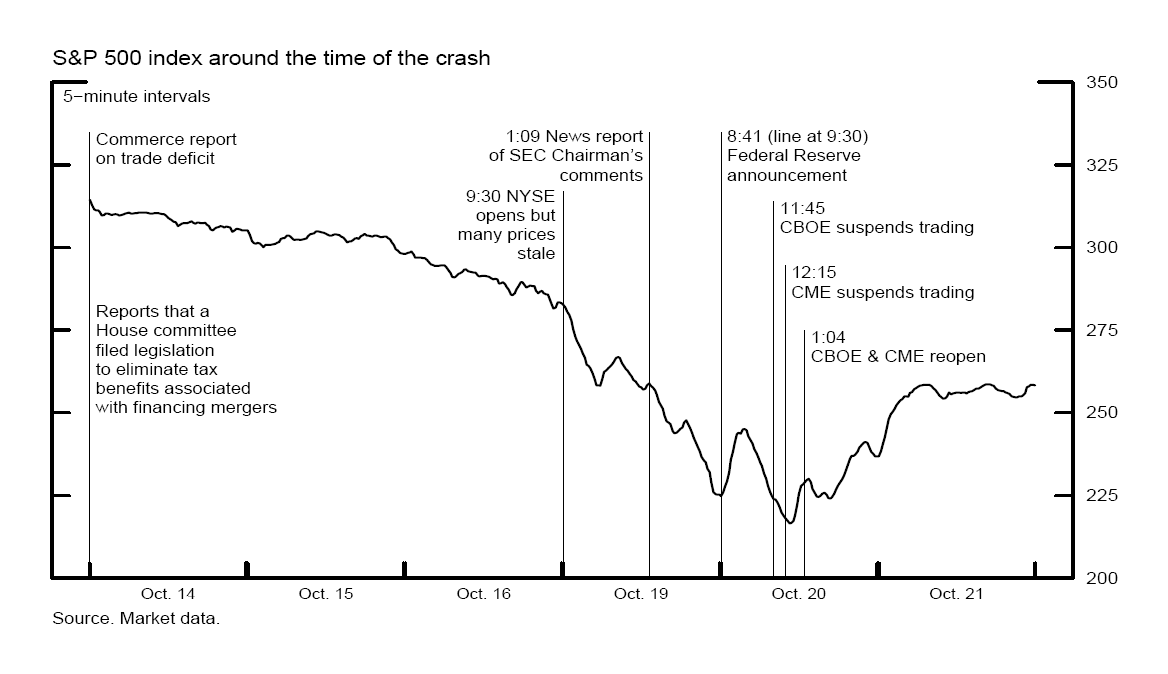
\includegraphics[height=0.36\textheight]{ch9_crash_1987.png}\\[1mm]
\imgcap{S\&P 500 în jurul datei de 19 octombrie 1987}
\imgcredit{https://commons.wikimedia.org/wiki/File:S\%26P_500_index_around_the_time_of_the_crash.png}{Figură: Mark Carlson, Federal Reserve Board (2006); domeniu public; Wikimedia Commons}
\end{column}
\begin{column}{0.56\textwidth}
\begin{itemize}
    \item 1987: o cădere de circa 20\% într-o singură zi pe piața acțiunilor din SUA arată că solvabilitatea o decide coada, nu varianța
    \item 1996: Comitetul de la Basel adoptă VaR pentru riscul de piață și un backtest de tip semafor pentru depășiri \refBCBS
    \item 1999--2002: VaR nu este coerent; ES este coerent \refADEH, \refAT
    \item 2011--2016: ES nu este elicitabil \refGn, dar perechea (VaR, ES) este elicitabilă împreună \refFZ
    \item FRTB: capitalul pe baza ES 2,5\%, backtesting pe VaR 1\% și VaR 2,5\% \refMAR
\end{itemize}
\end{column}
\end{columns}
\end{frame}

\begin{frame}{Basel: prognozatorul și arbitrul}
\itemsize{\small}
\begin{columns}[T]
\begin{column}{0.36\textwidth}
\centering
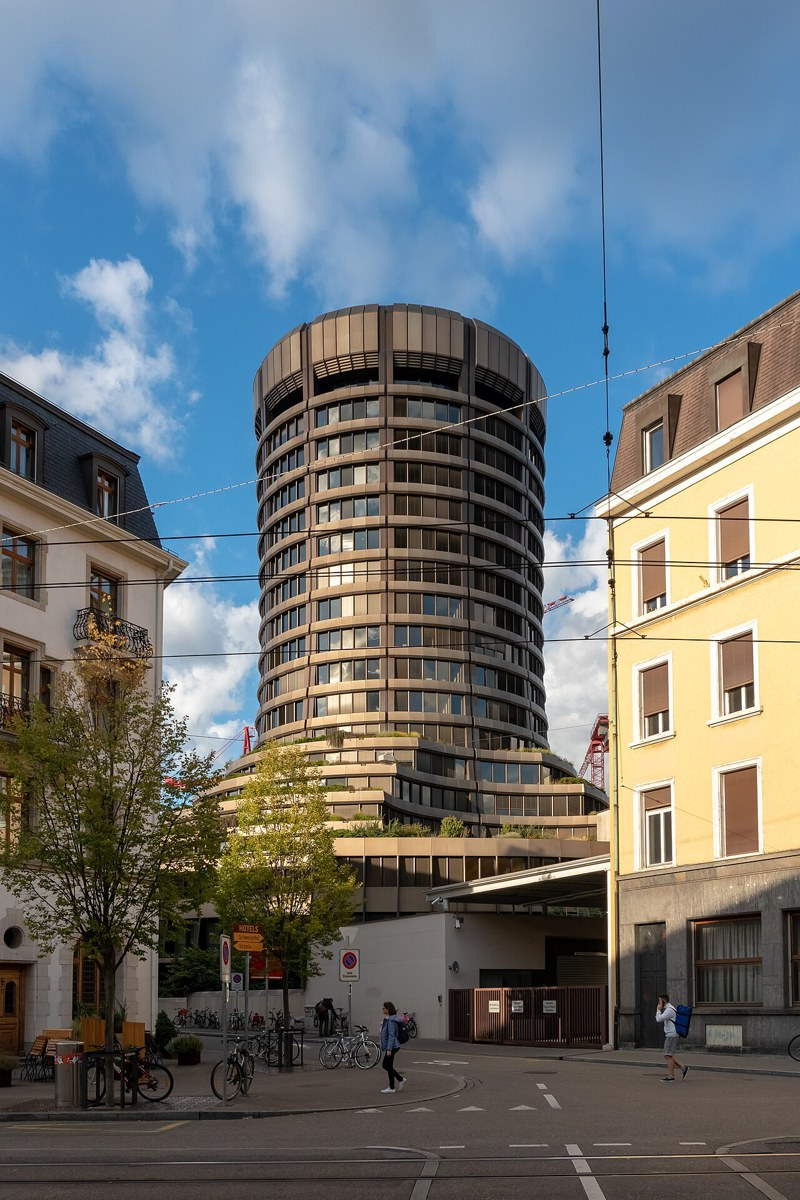
\includegraphics[height=0.5\textheight]{ch9_bis_basel_2018.jpg}\\[1mm]
\imgcap{Banca Reglementelor Internaționale, Basel, 2018}
\imgcredit{https://commons.wikimedia.org/wiki/File:Bank_for_International_Settlements_in_the_late_afternoon.jpg}{Foto: Michal Pleskowicz (2018); CC BY-SA 4.0; Wikimedia Commons}
\end{column}
\begin{column}{0.62\textwidth}
\begin{itemize}
    \item O bancă emite zilnic o prognoză a propriei cozi; supraveghetorul o verifică ulterior
    \item Două întrebări pe care statistica le separă: este prognoza \textbf{calibrată} (backtesting) și este ea \textbf{mai bună} decît alta (comparație)?
    \item Elicitabilitatea decide care prognoze pot fi comparate \refNZ
    \item Contează stimulentul: o regulă de scor răsplătește raportarea onestă doar dacă este strict consistentă pentru țintă
\end{itemize}
\end{column}
\end{columns}
\end{frame}


%=============================================================================
\section{Măsurile de risc ca funcționale de prognoză}
%=============================================================================

\begin{frame}{Cunoscut din TSA și MFM și elemente noi}
\itemsize{\small}
\begin{itemize}
    \item Cunoscut: VaR și ES prin simulare istorică, metode parametrice, FHS și EVT; testele Kupiec și Christoffersen; semaforul Basel (\atschlink{https://danpele.github.io/Time-Series-Analysis/RO/Cursuri/capitol5_volatilitate_conditionata_garch.pdf}{TSA, Capitolul 5}; MFM, Capitolele 7--8)
    \item Nou: perspectiva prognozei
    \begin{itemize}
        \item ce pierderi sînt consistente pentru o cuantilă și pentru perechea (VaR, ES); ce aduce elicitabilitatea și ce nu aduce
        \item M-estimarea modelelor dinamice de cuantilă și de ES: identificare, asimptotică, funcții obiectiv nenetede
        \item backtesting ca teste de momente ale calibrării condiționate, cu risc de estimare; comparații valide sub testare multiplă
    \end{itemize}
    \item Replicări: Engle și Manganelli (2004) și Patton, Ziegel și Chen (2019), cu specificațiile din lucrări, pe datele noastre
\end{itemize}
\end{frame}

\begin{frame}{VaR și ES ca funcționale}
\itemsize{\small}
\begin{itemize}
    \item Randamentul $Y$ cu distribuția $F$; nivelul $\alpha$ (VaR 1\%: $\alpha = 0{,}01$); cuantila $q_\alpha(F) = \inf\{y: F(y) \ge \alpha\}$
    \begin{itemize}
        \item $\mathrm{VaR}_\alpha(F) = -q_\alpha(F)$; rata de depășire țintă $\Pr(Y < -\mathrm{VaR}_\alpha) = \alpha$
    \end{itemize}
    \item $\mathrm{ES}_\alpha(F) = -\dfrac{1}{\alpha}\displaystyle\int_0^\alpha q_u(F)\,du$ \refAT; pentru $F$ continuă: $\mathrm{ES}_\alpha = -\E[Y \mid Y \le q_\alpha]$
    \begin{itemize}
        \item ES este coerent (subaditiv) \refADEH; VaR nu este; ES cere $\E|Y| < \infty$
    \end{itemize}
    \item În formule lucrăm cu perechea pe scala randamentelor $(v, e) = (q_\alpha, -\mathrm{ES}_\alpha)$, ambele negative: $e \le v < 0$
    \item Ambele sînt \textbf{funcționale} $\mathrm T(F)$: o prognoză a lor este o prognoză punctuală a distribuției predictive, ca în \atschlink{https://danpele.github.io/Advanced-Time-Series/RO/Cursuri/capitol1_evaluarea_prognozelor.pdf}{Capitolul 1}
\end{itemize}
\end{frame}

\begin{frame}{Prognoze condiționate de risc: trei căi}
\itemsize{\small}
\begin{itemize}
    \item Ținta: $(v_t, e_t) = \mathrm T(F_{t|t-1})$, unde $F_{t|t-1}$ este distribuția lui $Y_t$ condiționată de $\mathcal F_{t-1}$
    \item \textbf{Poziție--scală}: $Y_t = \mu_t + \sigma_t\eta_t$, $\eta_t$ i.i.d.\ $\Rightarrow v_t = \mu_t + \sigma_t q_\alpha(\eta)$, $e_t = \mu_t + \sigma_t\E[\eta \mid \eta \le q_\alpha(\eta)]$
    \begin{itemize}
        \item GARCH cu inovații din distribuția Normală, t asimetrică \refHan\ sau empirice (EDF); raportul $e_t/v_t$ este atunci constant în timp
    \end{itemize}
    \item \textbf{Dinamica directă a cuantilei}: $v_t = v(\mathcal F_{t-1}; \beta)$ estimat prin pierderea cuantilică, fără distribuție \refEM
    \item \textbf{Semiparametric comun}: $(v_t, e_t) = (v, e)(\mathcal F_{t-1}; \theta)$ estimat printr-o pierdere Fissler--Ziegel \refPZC, \refDB
    \item Fiecare cale produce o prognoză punctuală a unei funcționale; funcția de scor din secțiunea următoare le face comparabile
\end{itemize}
\end{frame}

\begin{frame}{Treizeci și șase de ani de prognoze ale cozii}
\itemsize{\footnotesize}
\begin{center}
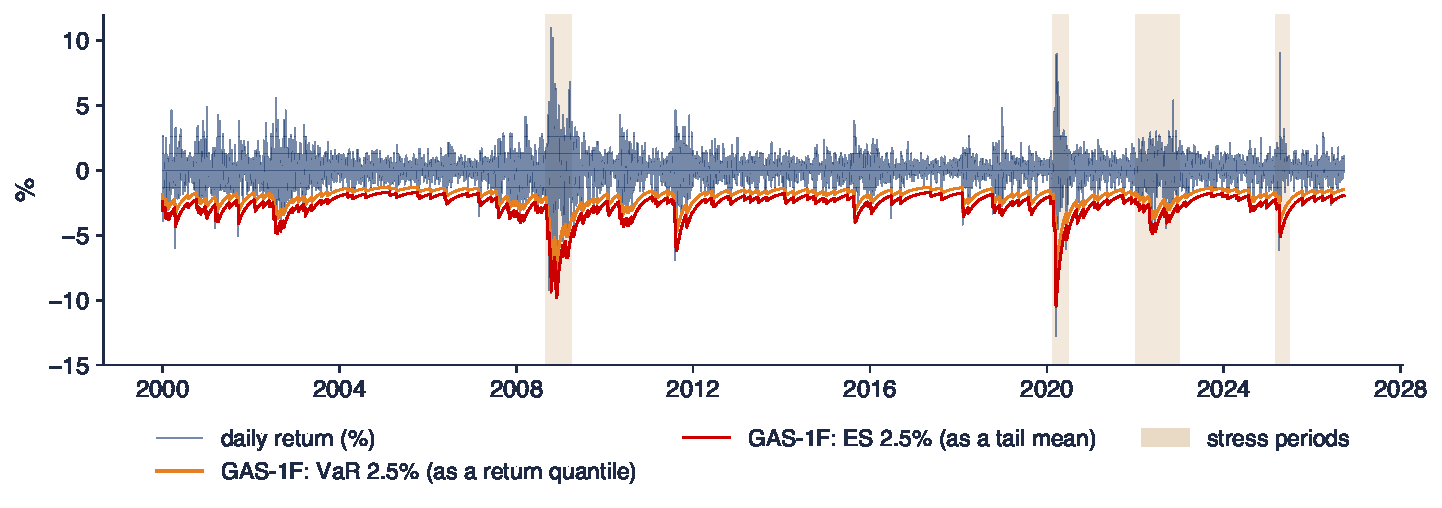
\includegraphics[width=0.97\textwidth,height=0.5\textheight,keepaspectratio]{ats_ch9_overview.pdf}
\end{center}
\vspace{-0.25cm}
\begin{itemize}
    \item Randamentele zilnice ale S\&P 500; modelul GAS-1F al lui Patton, Ziegel și Chen, cu parametrii estimați o singură dată pe 1990--1999 și apoi doar filtrați; zonele colorate: cele patru perioade de criză
\end{itemize}
\quantlet{ATS\_ch9\_pzc}{\qlurl{ATS_ch9_pzc}}
\end{frame}

\begin{frame}{Interpretarea prognozelor pe termen lung}
\itemsize{\small}
\begin{itemize}
    \item Prognoza ES 2,5\% variază de la circa \ensuremath{-}2{,}44\% (mediana) la \ensuremath{-}10{,}5\% la 17 martie 2020: riscul de coadă se mișcă la fel de mult ca volatilitatea
    \item Prognozele reacționează doar în zilele cu depășiri și scad lin în rest: actualizarea prin scor a modelului GAS
    \item Parametrii fixați în 1999 urmăresc încă anii 2008, 2020 și 2025: dinamica se generalizează, nivelul nu cere reestimare
    \item Dacă aceasta este suficient este o întrebare de testare (secțiunile 5--6), nu una vizuală
\end{itemize}
\end{frame}

\begin{frame}{Recapitulare: măsurile de risc ca funcționale}
\itemsize{\small}
\begin{itemize}
    \item VaR este o cuantilă, ES o integrală de cuantile; ambele sînt funcționale ale distribuției predictive
    \item Trei căi: poziție--scală, dinamica directă a cuantilei, modele semiparametrice comune
    \item Convenția: VaR 1\%, ES 2,5\%, $\alpha$ este rata de depășire țintă
\end{itemize}
\end{frame}


%=============================================================================
\section{Elicitabilitate și funcții de scor}
%=============================================================================

\begin{frame}{Consistență, elicitabilitate, identificare}
\itemsize{\small}
\begin{itemize}
    \item O funcție de scor $S(x, y)$ este \textbf{consistentă} pentru $\mathrm T$ pe o clasă $\mathcal F$ dacă $\E_F S(\mathrm T(F), Y) \le \E_F S(x, Y)$ pentru orice $x$ și $F \in \mathcal F$; \textbf{strict} dacă egalitatea impune $x = \mathrm T(F)$ \refGn
    \begin{itemize}
        \item $\mathrm T$ este \textbf{elicitabilă} dacă există o funcție $S$ strict consistentă (\atschlink{https://danpele.github.io/Advanced-Time-Series/RO/Cursuri/capitol1_evaluarea_prognozelor.pdf}{Capitolul 1})
    \end{itemize}
    \item \textbf{Funcție de identificare}: $V(x, y)$ cu $\E_F V(x, Y) = 0 \iff x = \mathrm T(F)$
    \begin{itemize}
        \item cuantila: $V(x, y) = \mathbf 1\{y \le x\} - \alpha$; media: $V(x, y) = x - y$
        \item Principiul lui Osband: $\partial_x\E_F S(x, Y) = h(x)\,\E_F V(x, Y)$, $h > 0$; scorurile sînt funcții de identificare integrate \refFZ
    \end{itemize}
    \item Funcțiile de identificare dau \textbf{backtesting} (este prognoza calibrată?); funcțiile de scor dau \textbf{comparații} (care prognoză este mai bună?) \refNZ
\end{itemize}
\end{frame}

\begin{frame}{Cuantilele: toate scorurile consistente}
\itemsize{\small}
\begin{itemize}
    \item \textbf{Teoremă} \refGn: în condiții slabe, $S$ este consistentă pentru $q_\alpha$ dacă și numai dacă $S(x, y) = (\mathbf 1\{y \le x\} - \alpha)(G(x) - G(y))$, cu $G$ nedescrescătoare (liniară pe porțiuni generalizată, GPL)
    \begin{itemize}
        \item $G(x) = x$: pierderea pinball; $G$ strict crescătoare dă consistența strictă
    \end{itemize}
    \item Motivul: $\partial_x\E_F S(x, Y) = G'(x)\,(F(x) - \alpha)$, negativă sub $q_\alpha$, pozitivă deasupra (\atsapplink{atsapp1}{atssrc1}{Anexă})
    \begin{itemize}
        \item $G(x) = \ln x$ pentru variabile pozitive dă un scor independent de scală (omogen de grad zero)
    \end{itemize}
    \item Funcții $G$ diferite dau aceeași prognoză optimă, dar pot ordona diferit două prognoze greșite: alegerea lui $G$ este o decizie de modelare
    \item Expectilele (pierdere pătratică asimetrică) sînt singurele măsuri de risc coerente și elicitabile \refZie; \refTayA\ le folosește pentru VaR și ES
\end{itemize}
\end{frame}

\begin{frame}{ES nu este elicitabil}
\itemsize{\small}
\begin{itemize}
    \item \textbf{Condiție necesară} \refGn: dacă $\mathrm T$ este elicitabilă, mulțimile ei de nivel $\{F: \mathrm T(F) = t\}$ sînt convexe
    \begin{itemize}
        \item demonstrație: dacă $\E_{F_0}S(t, Y) \le \E_{F_0}S(x, Y)$ și la fel pentru $F_1$, inegalitatea rămîne pentru $\lambda F_0 + (1 - \lambda)F_1$ (media este liniară în $F$)
    \end{itemize}
    \item Cuantilele trec testul: dacă $F_0(t) = F_1(t) = \alpha$, orice amestec are $F_\lambda(t) = \alpha$
    \item ES nu trece: amestecul schimbă cuantila, deci schimbă partea din fiecare componentă care intră în media cozii \refWeb
    \begin{itemize}
        \item consecință: nicio funcție de pierdere nu poate ordona prognoze ES singure; pierderile medii ale prognozelor ES nu au sens luate separat
    \end{itemize}
    \item Varianța nu trece din același motiv; perechile (medie, al doilea moment) și (VaR, ES) sînt elicitabile (\refFZ, „elicitabilitate de ordin superior”)
\end{itemize}
\end{frame}

\begin{frame}{Mulțimile de nivel la amestecare}
\itemsize{\footnotesize}
\begin{center}
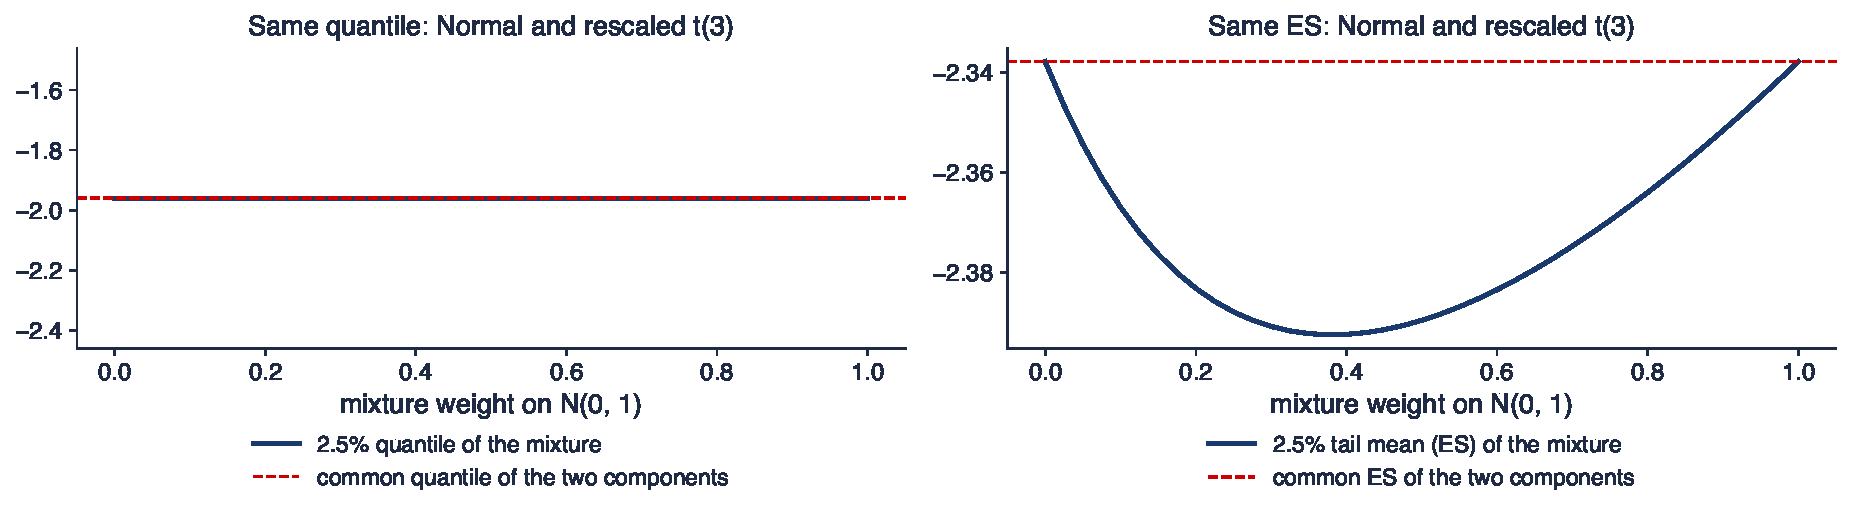
\includegraphics[width=0.97\textwidth,height=0.5\textheight,keepaspectratio]{ats_ch9_level_sets.pdf}
\end{center}
\vspace{-0.25cm}
\begin{itemize}
    \item Stînga: $N(0, 1)$ și o $t(3)$ rescalată la aceeași cuantilă de 2,5\%; dreapta: $N(0, 1)$ și o $t(3)$ rescalată la același ES 2,5\%; curbele: funcționala amestecului
\end{itemize}
\quantlet{ATS\_ch9\_scoring}{\qlurl{ATS_ch9_scoring}}
\end{frame}

\begin{frame}{Interpretarea mulțimilor de nivel}
\itemsize{\small}
\begin{itemize}
    \item Cuantila oricărui amestec rămîne \ensuremath{-}1{,}96: mulțimea de nivel a lui $q_{0{,}025}$ este convexă
    \item Ambele componente au media cozii \ensuremath{-}2{,}338; amestecul se îndepărtează cu pînă la 0{,}055 (la ponderea 0{,}38): mulțimea de nivel a ES nu este convexă
    \item Diferența este mică numeric, dar decisivă logic: un singur contraexemplu exclude orice pierdere strict consistentă pentru ES singur
    \item Soluția este prognoza cuantilei împreună cu ES: perechea are mulțimi de nivel convexe
\end{itemize}
\end{frame}

\begin{frame}{Elicitabilitatea comună: clasa Fissler--Ziegel}
\itemsize{\small}
\begin{itemize}
    \item \textbf{Teoremă} \refFZ, în forma din \refPZC, ec.~(4): pentru $e \le v$,
    \begin{itemize}
        \item $S(v, e, y) = (\mathbf 1\{y \le v\} - \alpha)\big(G_1(v) - G_1(y)\big) + G_2(e)\Big(v - e + \tfrac{1}{\alpha}\mathbf 1\{y \le v\}(y - v)\Big) - \mathcal G_2(e)$
        \item este consistentă pentru $(q_\alpha, -\mathrm{ES}_\alpha)$ dacă $G_1$ este nedescrescătoare și $\mathcal G_2' = G_2$ este pozitivă și crescătoare; strict consistentă în condiții slabe
    \end{itemize}
    \item Funcția de identificare a perechii: $V_1 = \mathbf 1\{y \le v\} - \alpha$, $V_2 = e - v + \tfrac{1}{\alpha}\mathbf 1\{y \le v\}(v - y)$
    \begin{itemize}
        \item $\E V_2 = 0$ la cuantila corectă este formula Acerbi--Tasche: ES este media cozii doar împreună cu cuantila corectă
    \end{itemize}
    \item Consecință \refFZG: ES poate fi \textbf{comparat} prin pereche; backtesting-ul clasic al ES cere în continuare mai mult decît ES (secțiunea 5)
\end{itemize}
\end{frame}

\begin{frame}{FZ0: membrul omogen de grad zero}
\itemsize{\small}
\begin{itemize}
    \item \refPZC, Propoziția 1: cu $v, e < 0$, \textbf{diferențele} de pierdere sînt invariante la rescalarea lui $Y$ dacă și numai dacă $G_1 = 0$, $G_2(e) = -1/e$:
    \begin{itemize}
        \item $L_{\mathrm{FZ0}}(y, v, e; \alpha) = -\dfrac{1}{\alpha e}\mathbf 1\{y \le v\}(v - y) + \dfrac{v}{e} + \ln(-e) - 1$
        \item partea de VaR seamănă cu pierderea pinball; partea de ES seamănă cu QLIKE (\atschlink{https://danpele.github.io/Advanced-Time-Series/RO/Cursuri/capitol8_volatilitate_avansata.pdf}{Capitolul 8})
    \end{itemize}
    \item De ce contează omogenitatea de grad zero pentru serii de timp
    \begin{itemize}
        \item cu un scor neomogen, zilele volatile domină pierderea medie și testul DM (diferențe de pierdere heteroscedastice)
        \item FZ0 ordonează la fel prognozele în \% și în puncte de bază; valoarea ei poate fi negativă (EUR/RON)
    \end{itemize}
    \item Contururile de pierdere așteptată constantă sînt convexe în condiții slabe, ceea ce ajută minimizarea numerică \refPZC
\end{itemize}
\end{frame}

\begin{frame}{Pierderile așteptate în jurul valorii corecte}
\itemsize{\footnotesize}
\begin{center}
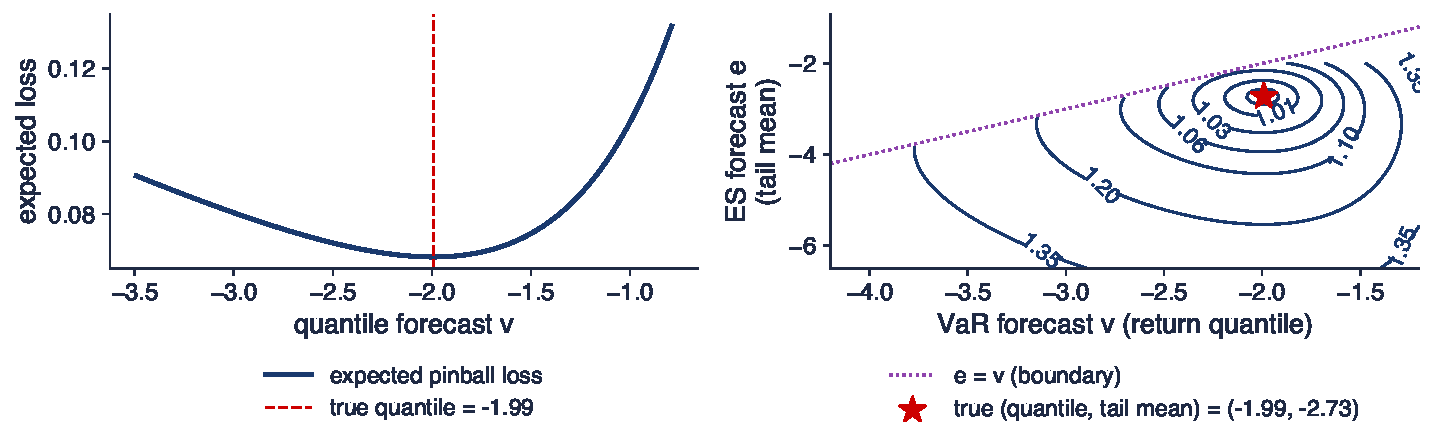
\includegraphics[width=0.97\textwidth,height=0.5\textheight,keepaspectratio]{ats_ch9_fz0_contour.pdf}
\end{center}
\vspace{-0.25cm}
\begin{itemize}
    \item Distribuția Student $t(5)$ cu varianță unitară, $\alpha = 0{,}025$, mediile prin simulare ($4\times10^5$ extrageri): stînga, pierderea pinball așteptată; dreapta, contururile pierderii FZ0 așteptate
\end{itemize}
\quantlet{ATS\_ch9\_scoring}{\qlurl{ATS_ch9_scoring}}
\end{frame}

\begin{frame}{Interpretarea pierderilor așteptate}
\itemsize{\small}
\begin{itemize}
    \item Curba pinball este minimă la \ensuremath{-}1{,}98, cuantila corectă fiind \ensuremath{-}1{,}99: consistența în acțiune
    \item Suprafața FZ0 este minimă în (\ensuremath{-}1{,}99; \ensuremath{-}2{,}73), cu minimul 1{,}004; contururile sînt convexe și alungite
    \item Ambele suprafețe sînt plate lîngă optim: diferențe mari între prognoze costă puțin în pierdere așteptată, deci testele cer multe zile din coadă
    \item Prognozele cu $e > v$ sînt inadmisibile: estimarea trebuie să impună ordinea
\end{itemize}
\end{frame}

\begin{frame}{Diagramele Murphy: ordonarea pentru toate scorurile consistente}
\itemsize{\small}
\begin{itemize}
    \item \refEGJK: orice scor GPL pentru cuantile este un amestec de \textbf{scoruri elementare}
    \begin{itemize}
        \item $S_\theta(x, y) = (\mathbf 1\{y < x\} - \alpha)\big(\mathbf 1\{\theta < x\} - \mathbf 1\{\theta < y\}\big)$, $\quad S(x, y) = \int S_\theta(x, y)\,dH(\theta)$
        \item $S_\theta$ este pierderea unei decizii binare cu pragul $\theta$; $H$ nedescrescătoare corespunde lui $G$
    \end{itemize}
    \item \textbf{Diagrama Murphy}: media $\bar S_\theta$ a fiecărei prognoze în funcție de $\theta$
    \begin{itemize}
        \item prognoza A domină B pentru orice scor consistent dacă și numai dacă curba ei este dedesubt pentru orice $\theta$
        \item curbe care se intersectează: ordonarea depinde de $G$, adică de pragurile care contează pentru utilizator
    \end{itemize}
    \item O verificare a ordonării pinball care costă o singură linie de cod
\end{itemize}
\end{frame}

\begin{frame}{O diagramă Murphy pentru VaR 2,5\%}
\itemsize{\footnotesize}
\begin{center}
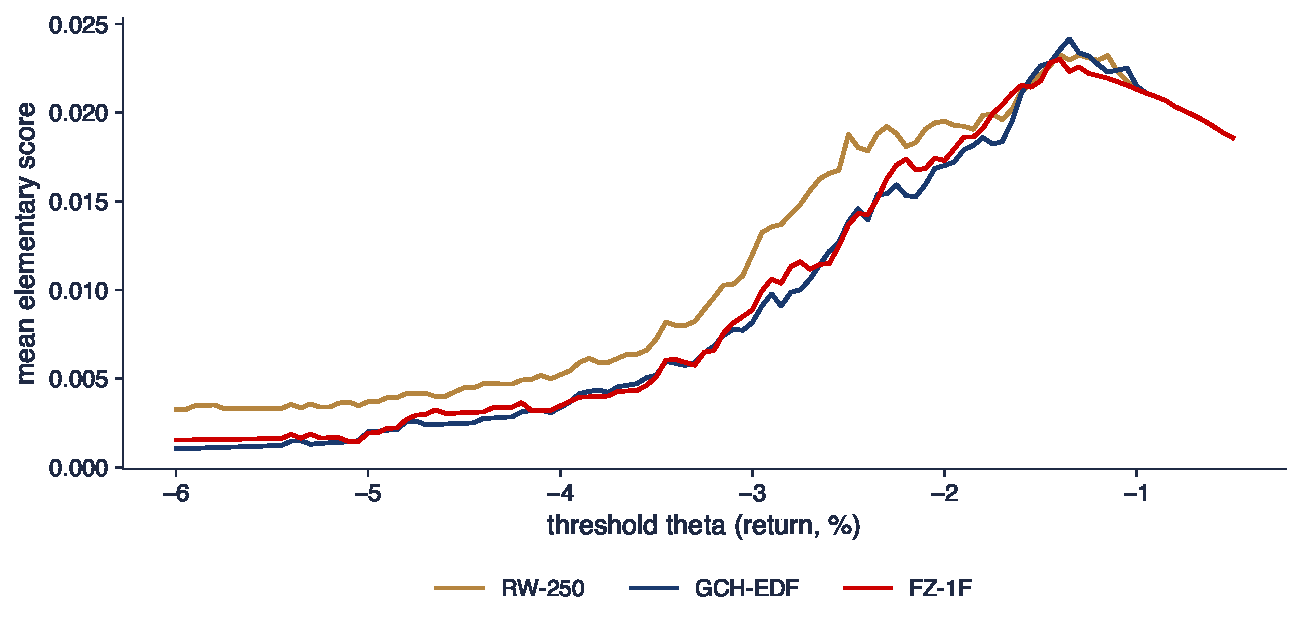
\includegraphics[width=0.97\textwidth,height=0.5\textheight,keepaspectratio]{ats_ch9_murphy.pdf}
\end{center}
\vspace{-0.25cm}
\begin{itemize}
    \item S\&P 500, în afara eșantionului 2000--2016 (designul PZC); scorurile elementare medii ale celor trei prognoze VaR 2,5\% în funcție de pragul $\theta$
\end{itemize}
\quantlet{ATS\_ch9\_scoring}{\qlurl{ATS_ch9_scoring}}
\end{frame}

\begin{frame}{Interpretarea diagramei Murphy}
\itemsize{\small}
\begin{itemize}
    \item GARCH-EDF este sub RW-250 la 91\% din praguri: prognoza dinamică domină aproape uniform
    \item GAS-1F și GARCH-EDF se intersectează: GAS-1F este mai bun doar la 38\% din praguri; pinball mediu 7{,}66 și 7{,}45 ($\times 10^{-2}$)
    \item Cele două modele bune diferă la pragurile adînci (sub $-4\%$), unde datele sînt puține
    \item O afirmație de tipul „modelul A este mai bun” trebuie să precizeze pentru ce scoruri; diagrama răspunde
\end{itemize}
\end{frame}

\begin{frame}{Recapitulare: elicitabilitate}
\itemsize{\small}
\begin{itemize}
    \item Scorurile compară, funcțiile de identificare testează; ambele provin din aceeași teorie
    \item Cuantilele: scoruri GPL; ES: nu singur; (VaR, ES): clasa Fissler--Ziegel
    \item FZ0 nu depinde de scală; diagramele Murphy verifică ordonarea pentru toate scorurile consistente
\end{itemize}
\end{frame}


%=============================================================================
\section{Regresia cuantilică și CAViaR}
%=============================================================================

\begin{frame}{Regresia cuantilică ca M-estimare}
\itemsize{\small}
\begin{columns}[T]
\begin{column}{0.27\textwidth}
\centering
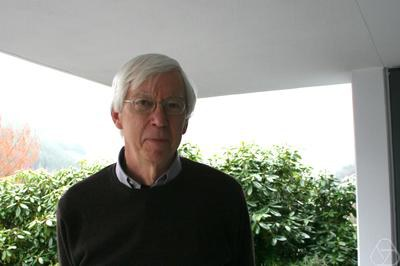
\includegraphics[height=0.26\textheight]{ch9_koenker_2012.jpg}\\[1mm]
\imgcap{Roger Koenker, Oberwolfach, 2012}
\imgcredit{https://commons.wikimedia.org/wiki/File:17224_Roger_W._Koenker.jpeg}{Foto: Ivonne Vetter, MFO (2012); CC BY-SA 2.0 de; Wikimedia Commons}
\end{column}
\begin{column}{0.71\textwidth}
\begin{itemize}
    \item \refKB: $\hat\beta(\alpha) = \arg\min_\beta \sum_t \rho_\alpha(y_t - x_t'\beta)$, o problemă de programare liniară
    \begin{itemize}
        \item condiția de ordinul întîi: $\sum_t x_t(\mathbf 1\{y_t \le x_t'\hat\beta\} - \alpha) \approx 0$, funcția de identificare
    \end{itemize}
    \item $\sqrt T(\hat\beta - \beta) \to N\big(0, \alpha(1 - \alpha)D^{-1}\Omega D^{-1}\big)$, $\Omega = \E[x_tx_t']$, $D = \E[f_t(q_t)x_tx_t']$ \refKoe
    \begin{itemize}
        \item densitatea condiționată în cuantilă (inversul „sparsity”) intră în $D$: se estimează cu un nucleu și o lățime de bandă
    \end{itemize}
    \item Serii de timp: autoregresia cuantilică \refKX\ permite coeficienților AR să varieze între cuantile; CAViaR face cuantila însăși autoregresivă
\end{itemize}
\end{column}
\end{columns}
\end{frame}

\begin{frame}{CAViaR: cele patru specificații}
\itemsize{\small}
\begin{columns}[T]
\begin{column}{0.3\textwidth}
\centering

\includegraphics[height=0.38\textheight]{ch9_engle_2022.jpg}\\[1mm]
\imgcap{Robert Engle, 2022}
\imgcredit{https://commons.wikimedia.org/wiki/File:0603-Kraneshares_KRBN-RobertEngle-JonDemske-13.jpg}{Foto: Jon Demske (2022); CC BY-SA 4.0; Wikimedia Commons}
\end{column}
\begin{column}{0.68\textwidth}
\begin{itemize}
    \item \refEM, scrise pentru $\mathrm{VaR}_t = -q_t(\alpha) > 0$:
    \item \textbf{SAV}: $\mathrm{VaR}_t = \beta_1 + \beta_2\mathrm{VaR}_{t-1} + \beta_3|y_{t-1}|$
    \item \textbf{AS}: $\mathrm{VaR}_t = \beta_1 + \beta_2\mathrm{VaR}_{t-1} + \beta_3(y_{t-1})^+ + \beta_4(y_{t-1})^-$
    \item \textbf{IG}: $\mathrm{VaR}_t = (\beta_1 + \beta_2\mathrm{VaR}_{t-1}^2 + \beta_3y_{t-1}^2)^{1/2}$ (un GARCH(1,1) cu inovații i.i.d.)
    \item \textbf{Adaptiv}: $\mathrm{VaR}_t = \mathrm{VaR}_{t-1} + \beta_1\big([1 + e^{G(y_{t-1} + \mathrm{VaR}_{t-1})}]^{-1} - \alpha\big)$, $G = 10$: crește după o depășire, scade lent în rest
    \item $\beta_2$ este persistența cozii; nu se presupune nicio distribuție
\end{itemize}
\end{column}
\end{columns}
\end{frame}

\begin{frame}{Estimare și inferență}
\itemsize{\small}
\begin{itemize}
    \item Criteriul de regresie cuantilică: $\hat\beta = \arg\min_\beta T^{-1}\sum_t \rho_\alpha\big(y_t + \mathrm{VaR}_t(\beta)\big)$; nediferențiabil și neconvex în $\beta$
    \begin{itemize}
        \item Procedura EM (secțiunea empirică): $\mathrm{VaR}_1$ = cuantila empirică din primele 300 de zile; $10^4$ vectori aleatori, cei mai buni 10 rafinați alternînd pași simplex și cvasi-Newton
    \end{itemize}
    \item Consistență și $\sqrt T(\hat\beta - \beta) \to N(0, \alpha(1 - \alpha)D^{-1}AD^{-1})$, $A = \E[\nabla q_t\nabla q_t']$, $D = \E[f_t(q_t)\nabla q_t\nabla q_t']$
    \begin{itemize}
        \item $\hat D = (2T\hat c)^{-1}\sum_t\mathbf 1\{|y_t - \hat q_t| < \hat c\}\nabla\hat q_t\nabla\hat q_t'$; luăm $\hat c$ din regula Hall--Sheather pe scala reziduurilor \refKoe
    \end{itemize}
    \item Gradienții $\nabla q_t$ urmează propria recursie (sau derivarea numerică a traiectoriei): modelul dinamic este un M-estimator recursiv
\end{itemize}
\end{frame}

\begin{frame}{Testul dinamic pe cuantile (DQ)}
\itemsize{\small}
\begin{itemize}
    \item $\mathrm{Hit}_t = \mathbf 1\{y_t < q_t\} - \alpha$: sub specificarea corectă este o diferență de martingală, $\E[\mathrm{Hit}_t \mid \mathcal F_{t-1}] = 0$
    \begin{itemize}
        \item regresăm $\mathrm{Hit}_t$ pe $X_t$ = (1, $\mathrm{Hit}_{t-1}, \dots, \mathrm{Hit}_{t-4}$, $q_t$), toate din $\mathcal F_{t-1}$ \refEM
    \end{itemize}
    \item În afara eșantionului: $\mathrm{DQ} = \dfrac{\mathrm{Hit}'X(X'X)^{-1}X'\mathrm{Hit}}{\alpha(1 - \alpha)} \to \chi^2_6$
    \begin{itemize}
        \item în eșantion, $\beta$ estimat face depășirile ortogonale pe gradienți: covarianța cere corecția derivată de EM
    \end{itemize}
    \item Testele Kupiec (doar constanta) și Christoffersen (o depășire întîrziată) sînt cazuri particulare; regresorul VaR adaugă putere împotriva erorilor care depind de nivel
    \item Cu $\alpha = 1\%$ și cîteva sute de zile, aproximarea $\chi^2$ este slabă (secțiunea 5): raportați valori $p$ simulate sau exacte cînd se poate
\end{itemize}
\end{frame}

\begin{frame}{Studiu de caz: Engle și Manganelli (2004) pe datele de azi}
\itemsize{\small}
\begin{itemize}
    \item Designul din secțiunea empirică a lucrării EM: 3\,392 de randamente zilnice, primele 2\,892 pentru estimare, ultimele 500 în afara eșantionului; VaR 1\% și 5\%
    \begin{itemize}
        \item EM au folosit 1986--1999 (GM, IBM, S\&P 500); noi folosim S\&P 500 de la 25 martie 2013 la 18 septembrie 2026, în afara eșantionului din 20 septembrie 2024
    \end{itemize}
    \item Aceleași specificații, valori de pornire și căutare; șocul tarifelor din aprilie 2025 cade în perioada din afara eșantionului
    \item Întrebări: ce specificație descrie coada de 1\%, sînt prognozele calibrate în afara eșantionului și este răspunsul la veștile proaste asimetric?
\end{itemize}
\end{frame}

\begin{frame}{VaR 1\% CAViaR pentru S\&P 500}
\itemsize{\footnotesize}
\begin{center}
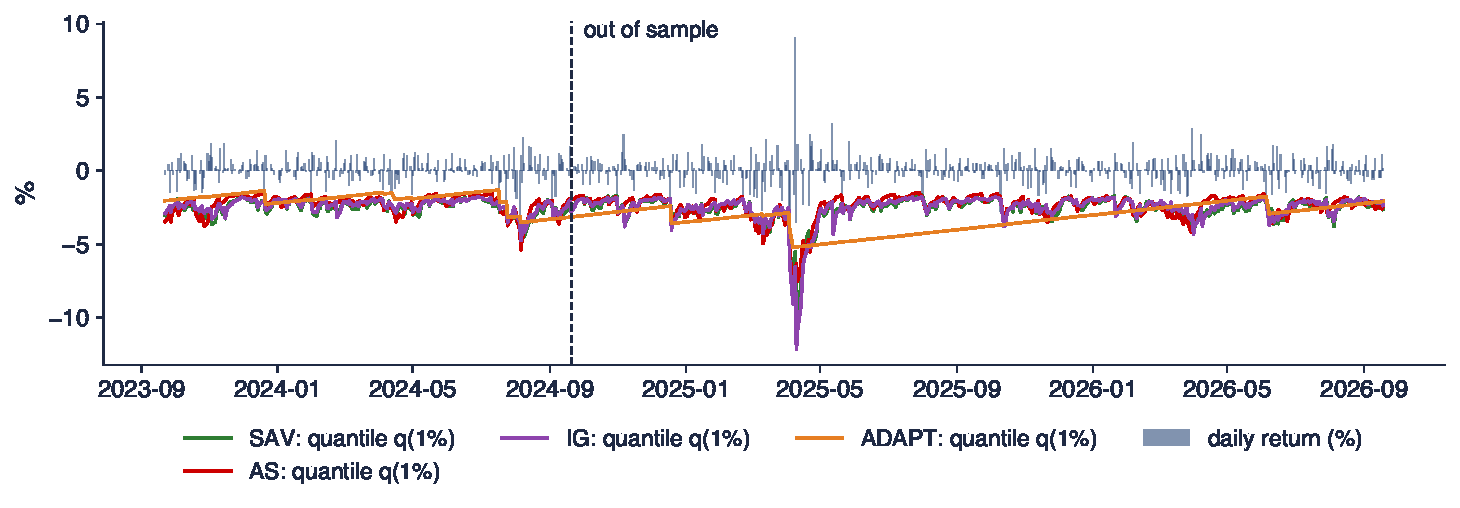
\includegraphics[width=0.97\textwidth,height=0.5\textheight,keepaspectratio]{ats_ch9_caviar.pdf}
\end{center}
\vspace{-0.25cm}
\begin{itemize}
    \item Ultimul an al eșantionului de estimare și cele 500 de zile din afara lui; liniile: cuantila de 1\% a randamentelor $q_t = -\mathrm{VaR}_t$ pentru cele patru specificații
\end{itemize}
\quantlet{ATS\_ch9\_caviar}{\qlurl{ATS_ch9_caviar}}
\end{frame}

\begin{frame}{Estimații, erori standard și teste DQ}
\itemsize{\footnotesize}
\begin{center}
\tiny
\begin{tabular}{lccccc>{\raggedright\arraybackslash}p{1.25cm}>{\raggedright\arraybackslash}p{1.35cm}>{\raggedright\arraybackslash}p{1.5cm}}
\toprule
\textbf{Modelul} & $\beta_1$ & $\beta_2$ & $\beta_3$ & $\beta_4$ & RQ$\times10^2$ & depășiri în eșantion (\%) & depășiri în afara eșantionului (\%) & DQ în afara eșantionului ($p$) \\
\midrule
SAV & 0{,}359 (0{,}217) & 0{,}702 (0{,}118) & 0{,}604 (0{,}243) & -- & 3{,}305 & 1{,}00 & 1{,}4 & 14{,}4 (0{,}025) \\
AS & 0{,}264 (0{,}137) & 0{,}805 (0{,}080) & 0{,}044 (0{,}185) & 0{,}616 (0{,}149) & 3{,}220 & 1{,}00 & 1{,}2 & 15{,}8 (0{,}015) \\
IG & 0{,}942 (0{,}467) & 0{,}674 (0{,}105) & 1{,}429 (0{,}702) & -- & 3{,}267 & 1{,}00 & 1{,}2 & 2{,}3 (0{,}891) \\
ADAPT & 1{,}190 (0{,}069) & -- & -- & -- & 4{,}044 & 0{,}90 & 0{,}8 & 27{,}5 ($<$0{,}001) \\
\bottomrule
\end{tabular}
\end{center}
\begin{itemize}
    \item Erorile standard din covarianța asimptotică EM; RQ: criteriul minimizat în eșantion; DQ în afara eșantionului cu patru depășiri întîrziate și VaR, $\chi^2_6$; 500 de zile dau 5 depășiri așteptate
    \item Pierderea pinball medie în afara eșantionului ($\times10^2$): SAV 3{,}87, AS 3{,}66, IG 3{,}66, adaptiv 4{,}42
\end{itemize}
\end{frame}

\begin{frame}{Interpretarea estimațiilor CAViaR}
\itemsize{\small}
\begin{itemize}
    \item Toate cele trei modele autoregresive reproduc rata din eșantion (circa 1\%) prin construcție: pierderea cuantilică calibrează nivelul
    \item AS: un randament negativ mută VaR de circa 14 ori mai mult decît unul pozitiv de aceeași mărime; $\beta_3$ nu se deosebește de zero
    \item În afara eșantionului IG trece testul DQ ($p$ = 0{,}891); SAV ($p$ = 0{,}025) și AS ($p$ = 0{,}015) sînt respinse la 5\%, modelul adaptiv clar ($p$ $<$0{,}001)
    \item Cinci depășiri așteptate în 500 de zile: respingerile vin din depășirile grupate din aprilie 2025, nu din numărul lor; o astfel de evidență este fragilă
    \item Modelul adaptiv reacționează doar la depășiri, ca un termostat lent: după grupul de depășiri din aprilie 2025 rămîne prea sus timp de luni de zile
\end{itemize}
\end{frame}

\begin{frame}{Curbele de impact al știrilor}
\itemsize{\footnotesize}
\begin{center}
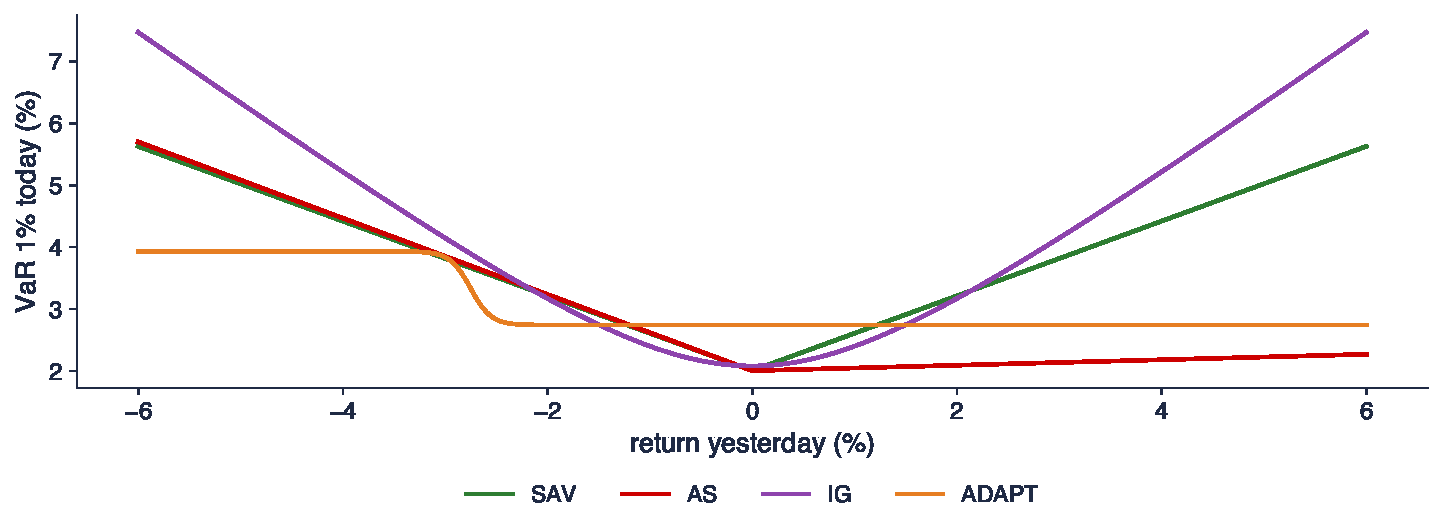
\includegraphics[width=0.97\textwidth,height=0.5\textheight,keepaspectratio]{ats_ch9_nic.pdf}
\end{center}
\vspace{-0.25cm}
\begin{itemize}
    \item $\mathrm{VaR}_t$ în funcție de $y_{t-1}$, cu $\mathrm{VaR}_{t-1}$ la mediana din eșantion (2{,}16\% pentru AS); parametrii estimați din tabel
\end{itemize}
\quantlet{ATS\_ch9\_caviar}{\qlurl{ATS_ch9_caviar}}
\end{frame}

\begin{frame}{Interpretarea curbelor de impact}
\itemsize{\small}
\begin{itemize}
    \item SAV și IG sînt simetrice prin construcție: o creștere de 5\% ridică VaR 1\% la fel de mult ca o cădere de 5\%
    \item AS este aproape plat pentru cîștiguri și abrupt pentru pierderi: efectul de levier estimat direct în coadă
    \item Curba adaptivă este o treaptă: contează doar semnul depășirii, nu mărimea ei
    \item Forma curbei este o restricție testabilă: AS include SAV ($\beta_3 = \beta_4$), un test Wald cu covarianța asimptotică EM
\end{itemize}
\end{frame}

\begin{frame}{Recapitulare: CAViaR}
\itemsize{\small}
\begin{itemize}
    \item Regresia cuantilică este M-estimare cu pierderea pinball; covarianța ei cere densitatea în cuantilă
    \item CAViaR face cuantila autoregresivă; estimarea cere multe puncte de pornire
    \item DQ testează depășirile față de informație; modelul asimetric descrie coada acțiunilor
\end{itemize}
\end{frame}


%=============================================================================
\section{Modele semiparametrice pentru (VaR, ES)}
%=============================================================================

\begin{frame}{M-estimarea cu pierderea FZ0}
\itemsize{\small}
\begin{itemize}
    \item Modelul $(v_t, e_t) = (v, e)(\mathcal F_{t-1}; \theta)$; estimatorul $\hat\theta = \arg\min_\theta T^{-1}\sum_t L_{\mathrm{FZ0}}(y_t, v_t(\theta), e_t(\theta); \alpha)$ \refPZC
    \begin{itemize}
        \item consistența rezultă din consistența strictă a FZ0 și din identificarea lui $\theta$; normalitatea asimptotică ca la CAViaR, cu o covarianță de tip sandwich
    \end{itemize}
    \item De ce nu verosimilitate maximă?
    \begin{itemize}
        \item Verosimilitatea maximă cere întreaga distribuție; un corp sau o coadă dreaptă greșite distorsionează estimațiile cozii stîngi
        \item Estimarea FZ țintește exact cele două funcționale de coadă: mai puțin eficientă dacă modelul este corect, robustă dacă nu este (PZC, Tabelele 3--4)
    \end{itemize}
    \item Înrudite: cvasi-verosimilitatea Laplace asimetrică \refTayB; regresiile pentru ES \refDB; dinamica determinată de scor (GAS) \refCKL
\end{itemize}
\end{frame}

\begin{frame}{Modelul GAS cu doi factori}
\itemsize{\small}
\begin{itemize}
    \item \refPZC, ec.~(9)--(16): $\begin{pmatrix} v_{t+1} \\ e_{t+1}\end{pmatrix} = w + B\begin{pmatrix} v_t \\ e_t\end{pmatrix} + A\lambda_t$, $B$ diagonală, $A$ o matrice $2\times2$
    \begin{itemize}
        \item variabilele de impuls din scorul FZ0: $\lambda_{v,t} = -v_t(\mathbf 1\{y_t \le v_t\} - \alpha)$, $\lambda_{e,t} = \tfrac{1}{\alpha}\mathbf 1\{y_t \le v_t\}y_t - e_t$
        \item ambele sînt funcții de identificare: medie condiționată nulă sub specificarea corectă
    \end{itemize}
    \item Hessiana se scalează cu $f_t(v_t) \approx k_\alpha/v_t$ (exact pentru randamente de tip poziție--scală), deci nu se estimează nicio densitate
    \item Opt parametri; în zilele fără depășire $\lambda_{e,t} = -e_t$, iar ambele măsuri de risc scad determinist spre mediile lor
\end{itemize}
\end{frame}

\begin{frame}{Modelele cu un factor, GARCH-FZ și Hybrid}
\itemsize{\small}
\begin{itemize}
    \item \textbf{GAS-1F}, ec.~(20): $v_t = a e^{\kappa_t}$, $e_t = b e^{\kappa_t}$, $b < a < 0$, $\kappa_t = \beta\kappa_{t-1} + \gamma\,\dfrac{-1}{e_{t-1}}\Big(\tfrac{1}{\alpha}\mathbf 1\{y_{t-1} \le v_{t-1}\}y_{t-1} - e_{t-1}\Big)$
    \begin{itemize}
        \item o singură log-scală latentă; termenul liber $\omega$ nu este identificat împreună cu $(a, b)$ și se fixează la 0
    \end{itemize}
    \item \textbf{GARCH-FZ}, ec.~(25)--(26): $\kappa_t^2 = 1 + \beta\kappa_{t-1}^2 + \gamma y_{t-1}^2$, $(v_t, e_t) = (a, b)\kappa_t$: un GARCH ajustat pentru coadă
    \item \textbf{Hybrid}, ec.~(27): GAS-1F plus $\delta\ln|y_{t-1}|$: reacționează în fiecare zi, mai puternic în zilele cu depășiri
    \item În toate trei raportul $e_t/v_t = b/a$ este constant: forma cozii este fixă, doar scala ei se mișcă
\end{itemize}
\end{frame}

\begin{frame}{Estimarea modelelor recursive nenetede}
\itemsize{\small}
\begin{itemize}
    \item Funcția obiectiv FZ0 este discontinuă în $\theta$ (prin $\mathbf 1\{y_t \le v_t(\theta)\}$), iar recursia propagă fiecare salt
    \item Anexa C a lucrării \refPZC: înlocuim indicatorul cu $\Gamma(y, v; \tau) = [1 + e^{\tau(y - v)}]^{-1}$ în pierdere și în variabila de impuls
    \begin{itemize}
        \item cvasi-Newton cu $\tau = 5$, apoi $\tau = 20$, apoi pierderea exactă cu metoda simplex, fiecare pas pornind din cel anterior
    \end{itemize}
    \item Valorile noastre de pornire: parametri dinamici aleatori, cu $(a, b)$ potriviți la VaR și ES din eșantion; cei mai buni patru sînt rafinați
    \item Restricții impuse prin penalizare: $e_t \le v_t$, $e_t < 0$, staționaritatea recursiei
\end{itemize}
\end{frame}

\begin{frame}{Studiu de caz: Patton, Ziegel și Chen (2019), secțiunea 5}
\itemsize{\small}
\begin{itemize}
    \item Date: randamentele zilnice ale S\&P 500, ianuarie 1990 -- decembrie 2016; estimare pe primii zece ani, parametrii păstrați ficși pentru 2000--2016 ($T = 4\,275$)
    \item Zece modele, ca în lucrare
    \begin{itemize}
        \item ferestre mobile de 125, 250 și 500 de zile (RW); ARMA (ordinul după BIC) -- GARCH(1,1) cu inovații din distribuția Normală, t asimetrică sau empirice
        \item GAS-2F, GAS-1F, GARCH-FZ și Hybrid estimate prin minimizarea FZ0
    \end{itemize}
    \item Rezultate replicate: pierderile FZ0 medii în afara eșantionului (Tabelul 8, $\alpha$ = 5\%; Tabelul S5, $\alpha$ = 2,5\%), statisticile DM (Tabelul 9), testele de adecvare (ec.~41)
    \item Datele noastre: închiderile EODHD ale aceluiași indice; diferențe de cîteva miimi sînt de așteptat din revizuiri ale datelor și din traseele optimizatorului
\end{itemize}
\end{frame}

\begin{frame}{Trei moduri de a prognoza coada}
\itemsize{\footnotesize}
\begin{center}
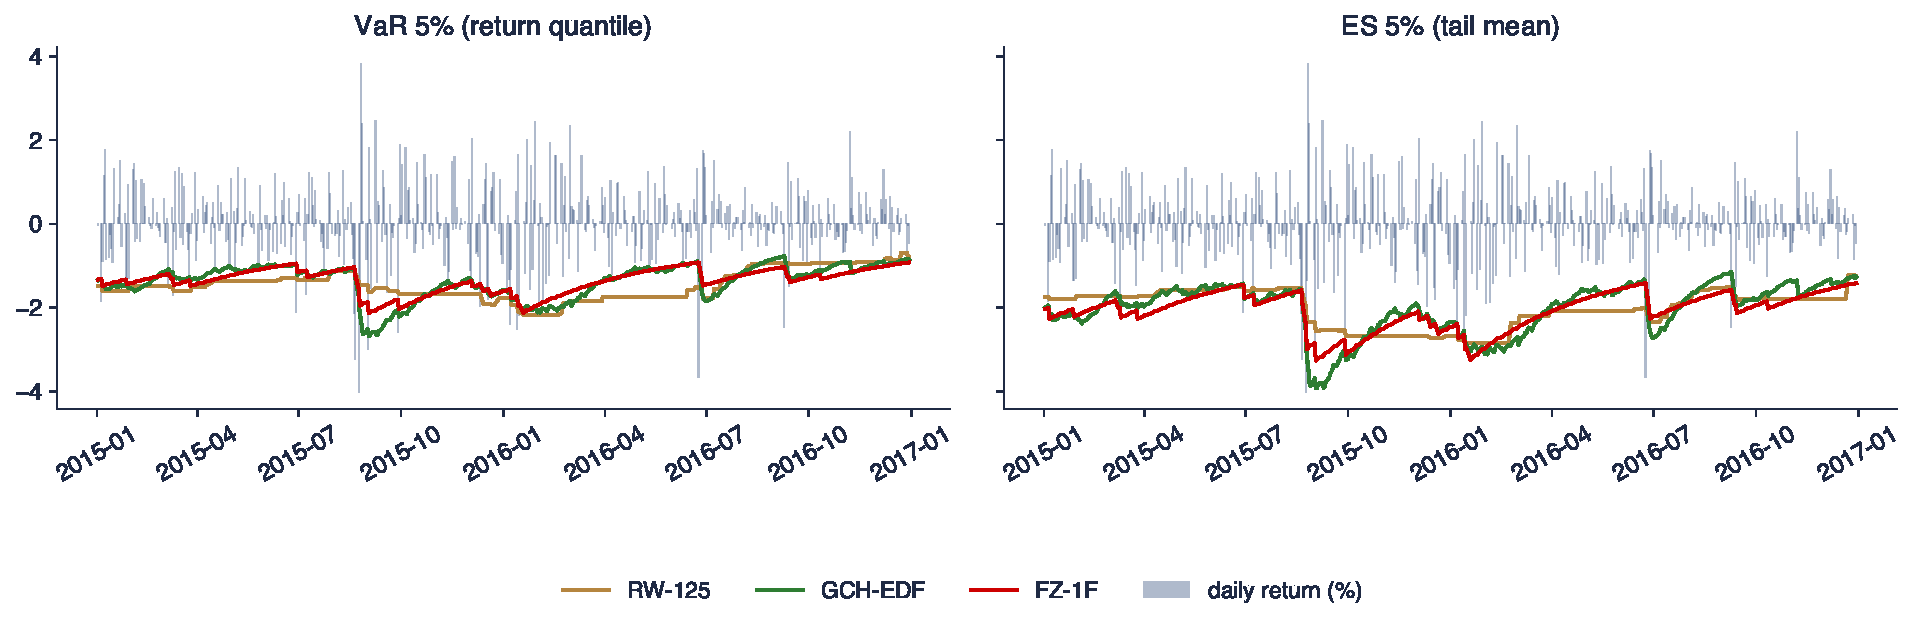
\includegraphics[width=0.97\textwidth,height=0.5\textheight,keepaspectratio]{ats_ch9_pzc_paths.pdf}
\end{center}
\vspace{-0.25cm}
\begin{itemize}
    \item VaR și ES 5\% pentru S\&P 500 în 2015--2016 (PZC, Figura 5 pe datele noastre): RW-125, GARCH-EDF și GAS-1F
\end{itemize}
\quantlet{ATS\_ch9\_pzc}{\qlurl{ATS_ch9_pzc}}
\end{frame}

\begin{frame}{Interpretarea celor trei prognoze}
\itemsize{\small}
\begin{itemize}
    \item Fereastra mobilă se mișcă în trepte, pe măsură ce zilele extreme intră și ies din fereastră, la luni după șoc
    \item GARCH-EDF se mișcă în fiecare zi cu pătratele randamentelor; GAS-1F se mișcă doar în zilele cu depășiri și apoi scade lin
    \item August 2015: GARCH reacționează cel mai mult, GAS-1F sare mai puțin, dar rămîne; în 2008, ES 5\% GAS-1F a ajuns la \ensuremath{-}9{,}9\%
    \item Ce reacție este corectă decide pierderea FZ0, nu aspectul traiectoriei
\end{itemize}
\end{frame}

\begin{frame}{Replicare: pierderea FZ0 medie în afara eșantionului}
\itemsize{\footnotesize}
\begin{center}
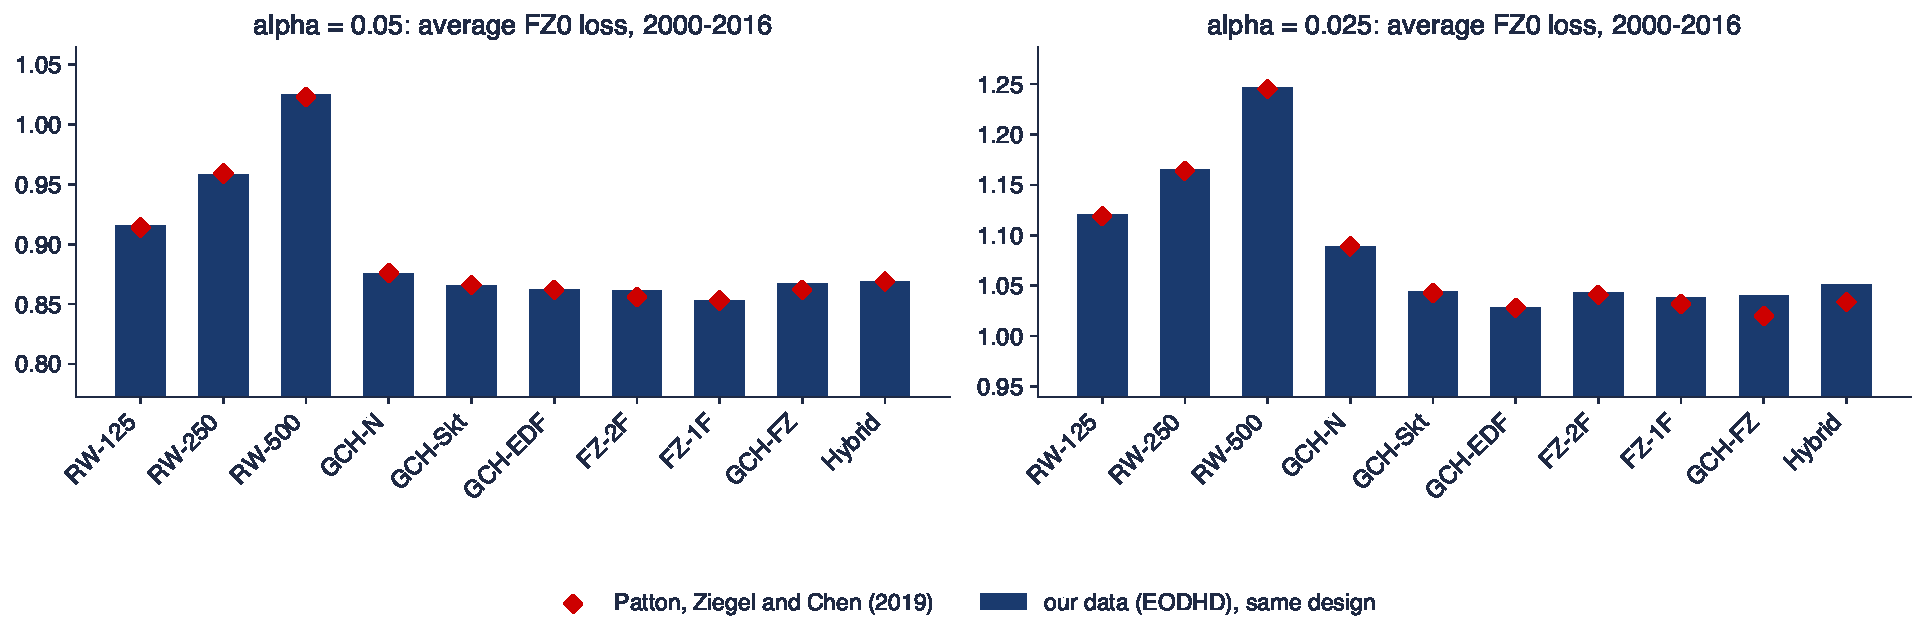
\includegraphics[width=0.97\textwidth,height=0.5\textheight,keepaspectratio]{ats_ch9_pzc_table.pdf}
\end{center}
\vspace{-0.25cm}
\begin{itemize}
    \item Bare: datele și codul nostru, același design; romburi: valorile tipărite în PZC, Tabelul 8 ($\alpha$ = 5\%) și Tabelul S5 ($\alpha$ = 2,5\%)
\end{itemize}
\quantlet{ATS\_ch9\_pzc}{\qlurl{ATS_ch9_pzc}}
\end{frame}

\begin{frame}{Replicarea în cifre}
\itemsize{\footnotesize}
\begin{center}
\scriptsize
\begin{tabular}{lcccccc}
\toprule
\textbf{Modelul} & \multicolumn{2}{c}{$\alpha = 5\%$} & \multicolumn{2}{c}{$\alpha = 2{,}5\%$} & \multicolumn{2}{c}{GoF $p$, $\alpha = 5\%$} \\ & noi & PZC & noi & PZC & VaR & ES \\
\midrule
RW-125 & 0{,}916 & 0{,}914 & 1{,}120 & 1{,}119 & 0{,}004 & 0{,}005 \\
RW-250 & 0{,}959 & 0{,}959 & 1{,}165 & 1{,}164 & $<$0{,}001 & 0{,}011 \\
RW-500 & 1{,}025 & 1{,}023 & 1{,}247 & 1{,}245 & $<$0{,}001 & $<$0{,}001 \\
GCH-N & 0{,}876 & 0{,}876 & 1{,}089 & 1{,}089 & 0{,}018 & $<$0{,}001 \\
GCH-Skt & 0{,}865 & 0{,}866 & 1{,}044 & 1{,}043 & 0{,}001 & 0{,}001 \\
GCH-EDF & 0{,}862 & 0{,}862 & 1{,}028 & 1{,}028 & 0{,}001 & 0{,}007 \\
FZ-2F & 0{,}862 & 0{,}856 & 1{,}044 & 1{,}041 & $<$0{,}001 & 0{,}003 \\
FZ-1F & 0{,}853 & 0{,}853 & 1{,}038 & 1{,}032 & 0{,}001 & 0{,}037 \\
GCH-FZ & 0{,}867 & 0{,}862 & 1{,}040 & 1{,}020 & 0{,}005 & 0{,}016 \\
Hybrid & 0{,}869 & 0{,}869 & 1{,}051 & 1{,}034 & $<$0{,}001 & $<$0{,}001 \\
\bottomrule
\end{tabular}
\end{center}
\begin{itemize}
    \item Cea mai mare diferență: 0{,}006 la 5\%, 0{,}020 la 2,5\%; BIC alege ARMA(0, 0) pentru medie (PZC: ARMA(1,1)); GARCH $\alpha$ = 0{,}052, $\beta$ = 0{,}942
\end{itemize}
\end{frame}

\begin{frame}{Interpretarea replicării}
\itemsize{\small}
\begin{itemize}
    \item Ordonarea din lucrare se reproduce: GAS-1F cel mai mic la 5\% (0{,}853, lucrarea 0{,}853), RW-500 cel mai slab, GARCH-N în urma celorlalte modele GARCH
    \item Estimațiile GAS-1F: $\beta$ = 0{,}995, $\gamma$ = \ensuremath{-}0{,}0069 (PZC, Tabelul 7: 0,990 și $-0{,}010$); Hybrid $\delta$ = 0{,}017 (0,018)
    \item Nereprodus: testele de adecvare; PZC găsesc că GAS-1F trece ($p$ 0,242 și 0,313), pe datele noastre este respins (0{,}001; 0{,}037)
    \item Pierderile medii sînt robuste la mici diferențe ale datelor; testele pe cîteva zile din coadă nu sînt, iar alegerea covarianței regresiei contează
\end{itemize}
\end{frame}

\begin{frame}{Teste Diebold--Mariano pe pierderile FZ0}
\itemsize{\footnotesize}
\begin{center}
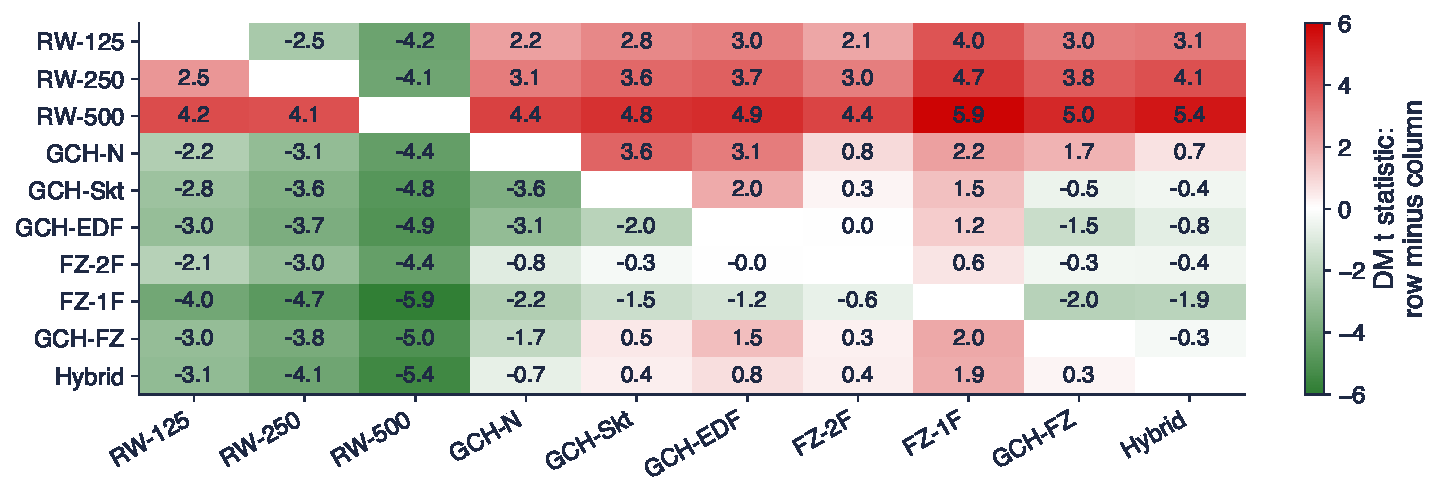
\includegraphics[width=0.97\textwidth,height=0.56\textheight,keepaspectratio]{ats_ch9_dm.pdf}
\end{center}
\vspace{-0.25cm}
\begin{itemize}
    \item S\&P 500, 2000--2016, $\alpha$ = 5\%: statistica DM a rîndului minus coloana, varianță Newey--West; roșu: modelul de pe rînd este mai slab (PZC, Tabelul 9)
\end{itemize}
\quantlet{ATS\_ch9\_pzc}{\qlurl{ATS_ch9_pzc}}
\end{frame}

\begin{frame}{Interpretarea matricei DM}
\itemsize{\small}
\begin{itemize}
    \item Coloana GAS-1F, noi față de PZC: RW-125 4{,}02 (3{,}91), RW-500 5{,}87 (5{,}48), GARCH-N 2{,}22 (1{,}99), GARCH-EDF 1{,}19 (1{,}20)
    \item Modelele cele mai slabe se separă ușor; primele cîteva nu (GARCH-Skt, GARCH-EDF, FZ-2F față de GAS-1F sub 1,96)
    \item O diferență: GARCH-FZ față de GAS-1F, 2{,}02 aici și 1{,}27 în lucrare; normalizarea scalei la GARCH-FZ face estimațiile fragile
    \item Nouăzeci de teste pe perechi cer un răspuns la testarea multiplă: MCS (secțiunea 6)
\end{itemize}
\end{frame}

\begin{frame}{Regresia comună (VaR, ES)}
\itemsize{\small}
\begin{itemize}
    \item \refDB: $q_\alpha(Y_t \mid x_t) = x_t'\beta$, $-\mathrm{ES}_\alpha(Y_t \mid x_t) = x_t'\gamma$, estimate împreună prin minimizarea unei pierderi Fissler--Ziegel
    \begin{itemize}
        \item M-estimator: consistent și asimptotic normal pentru orice membru al clasei; alegerea lui $(G_1, G_2)$ afectează doar eficiența
    \end{itemize}
    \item Utilizări
    \begin{itemize}
        \item ce variabile mișcă coada și cît: analogul pentru ES al regresiei cuantilice
        \item backtesting pentru ES: regresăm randamentele realizate pe prognoza ES și testăm termen liber 0, pantă 1 \refBD\ (\atschlink{https://danpele.github.io/MFM/RO/Cursuri/capitol8_backtesting_risc.pdf}{MFM, Capitolul 8})
    \end{itemize}
    \item Aplicație: randamentele S\&P 500 2000--2026 pe VIX-ul închiderii anterioare, $\alpha$ = 2,5\%, pierderea FZ0, erori standard prin bootstrap pe blocuri mobile (blocuri de 20 de zile)
\end{itemize}
\end{frame}

\begin{frame}{Coada S\&P 500 în funcție de VIX}
\itemsize{\footnotesize}
\begin{center}
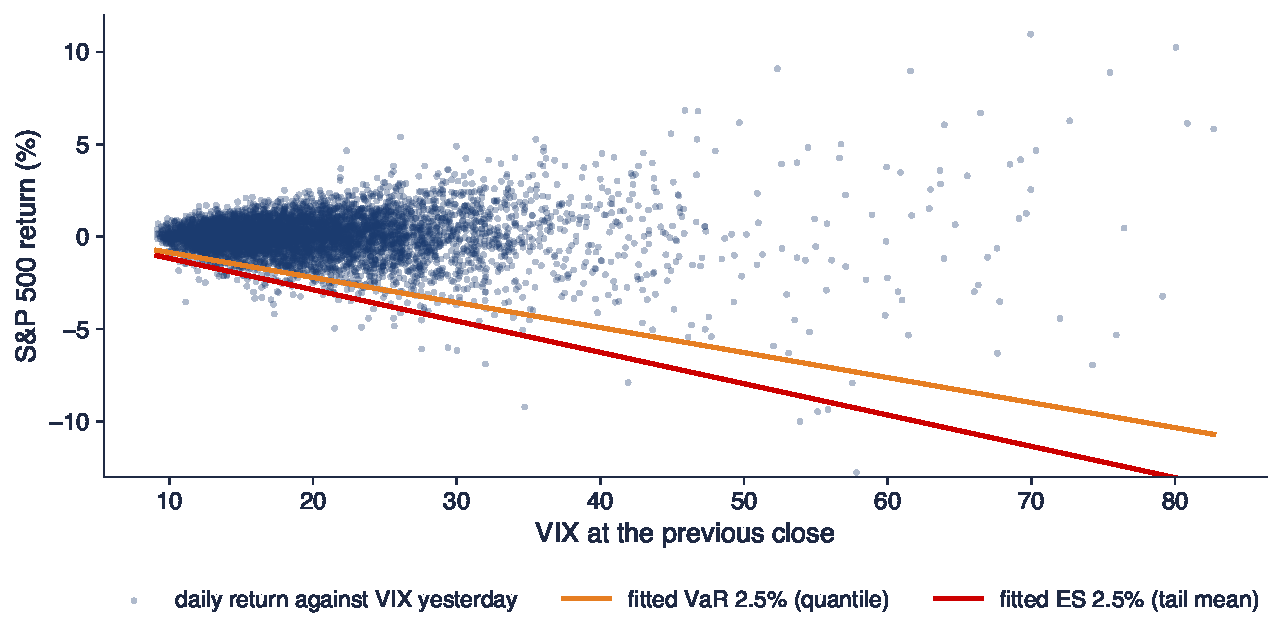
\includegraphics[width=0.97\textwidth,height=0.5\textheight,keepaspectratio]{ats_ch9_esreg.pdf}
\end{center}
\vspace{-0.25cm}
\begin{itemize}
    \item Randamentele zilnice în funcție de VIX-ul închiderii anterioare, $T = 6\,714$; liniile: cuantila de 2,5\% și media cozii estimate prin regresia comună
\end{itemize}
\quantlet{ATS\_ch9\_esreg}{\qlurl{ATS_ch9_esreg}}
\end{frame}

\begin{frame}{Interpretarea regresiei comune}
\itemsize{\small}
\begin{itemize}
    \item Cuantila: $0{,}499 \ensuremath{-}0{,}135\,\mathrm{VIX}$ (erori standard 0{,}150; 0{,}009); media cozii: $0{,}524 \ensuremath{-}0{,}170\,\mathrm{VIX}$ (erori standard 0{,}245; 0{,}015)
    \item Un punct de VIX coboară cuantila de 2,5\% cu 0{,}14 și media cozii cu 0{,}17 puncte procentuale: coada se deschide de 1{,}25 ori mai repede în ES
    \item Partea de cuantilă este apropiată de regresia cuantilică ($0{,}560$, $\ensuremath{-}0{,}139$); rata de depășire în eșantion 2{,}50\%; testele PZC nu resping ($p$ = 0{,}978; 0{,}744)
    \item VIX este o prognoză de piață a volatilității: regresia arată că piața opțiunilor evaluează coada stîngă aproape liniar
\end{itemize}
\end{frame}

\begin{frame}{Recapitulare: modelele semiparametrice (VaR, ES)}
\itemsize{\small}
\begin{itemize}
    \item Minimizarea FZ0 estimează perechea din coadă fără o distribuție
    \item Variabilele de impuls GAS sînt funcții de identificare: modelul se corectează doar cînd vorbește coada
    \item Ordonarea PZC se replică; rezultatele testelor de adecvare nu; regresia comună leagă coada de covariabile
\end{itemize}
\end{frame}


%=============================================================================
\section{Backtesting ca test de calibrare}
%=============================================================================

\begin{frame}{Recapitulare: numărarea depășirilor}
\itemsize{\small}
\begin{itemize}
    \item Depășirile $I_t = \mathbf 1\{y_t < v_t\}$; VaR corect $\Rightarrow I_t$ i.i.d.\ Bernoulli($\alpha$) (\atschlink{https://danpele.github.io/MFM/RO/Cursuri/capitol8_backtesting_risc.pdf}{MFM, Capitolul 8})
    \begin{itemize}
        \item \refKup: acoperirea necondiționată, LR $\sim \chi^2_1$; \refChr: independența depășirilor consecutive și acoperirea condiționată, $\chi^2_2$
        \item Semaforul Basel \refBCBS: verde pînă la 4 depășiri ale VaR 1\% în 250 de zile, galben 5--9, roșu de la 10
    \end{itemize}
    \item Ce nu vede numărarea
    \begin{itemize}
        \item depășirile care depind de altă informație decît ultima depășire (DQ)
        \item mărimea pierderilor din coadă (backtesting pentru ES); distanța dintre depășiri (teste de durată)
        \item efectul parametrilor estimați asupra distribuției sub ipoteza nulă
    \end{itemize}
\end{itemize}
\end{frame}

\begin{frame}{Calibrarea condiționată}
\itemsize{\small}
\begin{itemize}
    \item O prognoză $x_t$ a lui $\mathrm T$ este \textbf{calibrată condiționat} dacă $\E[V(x_t, Y_t) \mid \mathcal F_{t-1}] = 0$, unde $V$ este funcția de identificare \refNZ
    \begin{itemize}
        \item pentru orice instrumente $h_{t-1} \in \mathcal F_{t-1}$: $\E[h_{t-1}V(x_t, Y_t)] = 0$, un test de momente (Wald, $\chi^2$)
    \end{itemize}
    \item PZC, ec.~(40)--(41): reziduurile generalizate standardizate $\lambda^s_{v,t} = \mathbf 1\{y_t \le v_t\} - \alpha$ și $\lambda^s_{e,t} = \dfrac{\mathbf 1\{y_t \le v_t\}y_t}{\alpha e_t} - 1$
    \begin{itemize}
        \item regresăm fiecare pe (1, propriul decalaj, $v_t$ sau $e_t$) și testăm că toți cei trei coeficienți sînt zero; folosim covarianța White (HC0)
    \end{itemize}
    \item DQ este cazul particular pentru VaR; regresia pentru ES testează ES doar împreună cu VaR, cum prevede elicitabilitatea
    \item Puterea vine din instrumente: depășirile întîrziate detectează gruparea, nivelul prognozei detectează erorile de scală
\end{itemize}
\end{frame}

\begin{frame}{Teste pe baza duratelor}
\itemsize{\small}
\begin{itemize}
    \item \refCP: pentru un VaR corect, duratele $d_i$ dintre depășiri sînt geometrice, fără memorie, cu media $1/\alpha$
    \begin{itemize}
        \item alternativa: hazardul Weibull $\lambda(d) = a^b b\,d^{b-1}$; $b < 1$ înseamnă hazard descrescător, adică depășirile se grupează
    \end{itemize}
    \item Verosimilitatea cu cenzurare: primul și ultimul interval sînt incomplete și intră prin funcția de supraviețuire $S(d) = e^{-(ad)^b}$
    \begin{itemize}
        \item $\mathrm{LR} = 2[\ln L(\hat a, \hat b) - \ln L(\tilde a, 1)] \to \chi^2_1$; pentru eșantioane mici se recomandă valori $p$ prin simulare
    \end{itemize}
    \item Duratele văd gruparea la orice distanță, nu doar în zile consecutive, ca testul lui Christoffersen
\end{itemize}
\end{frame}

\begin{frame}{Cît de departe sînt depășirile una de alta?}
\itemsize{\footnotesize}
\begin{center}
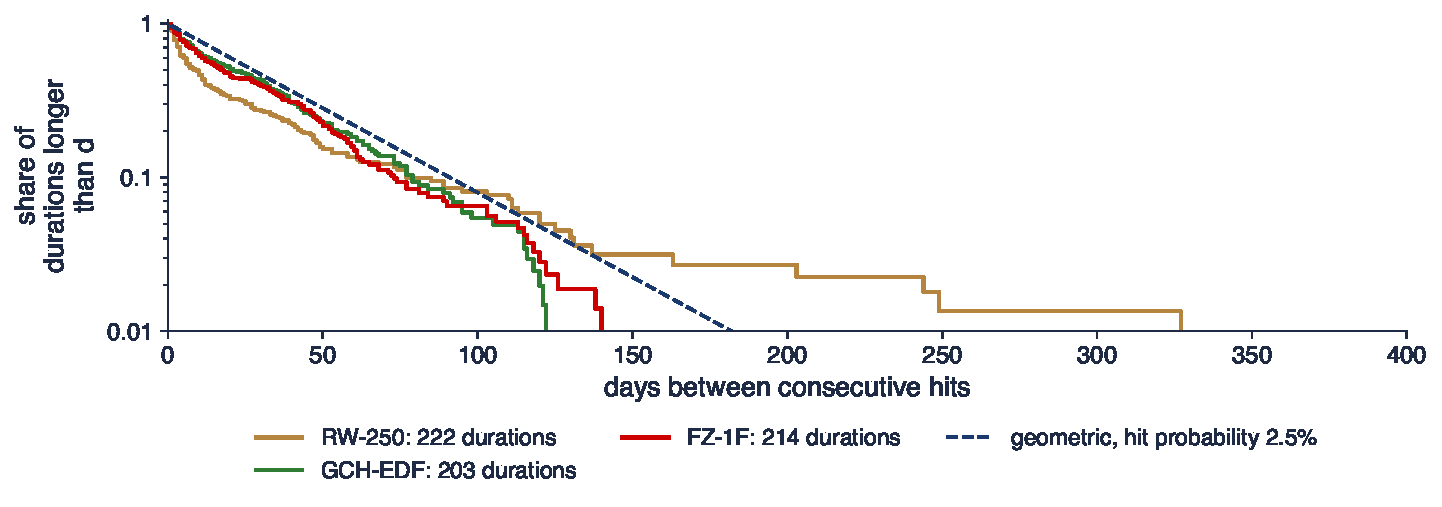
\includegraphics[width=0.97\textwidth,height=0.5\textheight,keepaspectratio]{ats_ch9_durations.pdf}
\end{center}
\vspace{-0.25cm}
\begin{itemize}
    \item S\&P 500, VaR 2,5\%, în afara eșantionului 2000--2026; funcția de supraviețuire empirică a duratelor dintre depășiri (scară logaritmică) față de legea geometrică a unui model corect
\end{itemize}
\quantlet{ATS\_ch9\_backtests}{\qlurl{ATS_ch9_backtests}}
\end{frame}

\begin{frame}{Interpretarea duratelor}
\itemsize{\small}
\begin{itemize}
    \item RW-250: 40\% din durate sînt de cel mult 5 zile (geometric: 12\%); Weibull $b$ = 0{,}67, $p$ $<$0{,}001: grupare puternică
    \item GARCH-EDF: $b$ = 0{,}92, $p$ = 0{,}107; GAS-1F: $b$ = 0{,}88, $p$ = 0{,}019: modelele dinamice elimină cea mai mare parte a grupării
    \item Coada lungă a RW-250 (ani calmi fără depășiri) este cealaltă față a grupării: fereastra își amintește crizele vechi
    \item Toate modelele au prea multe depășiri în total (tabelul din secțiunea 5): parametrii fixați în 1999 sînt prea optimiști după 2000
\end{itemize}
\end{frame}

\begin{frame}{Backtesting pentru ES: ce cere fiecare test}
\itemsize{\footnotesize}
\begin{center}
\scriptsize
\begin{tabular}{>{\raggedright\arraybackslash}p{3.2cm}>{\raggedright\arraybackslash}p{4.5cm}>{\raggedright\arraybackslash}p{3.8cm}}
\toprule
\textbf{Testul} & \textbf{Statistica} & \textbf{Date necesare} \\
\midrule
\refMF{} & media lui $(y_t - e_t)/\sigma_t$ în zilele cu depășiri, bootstrap & $v_t$, $e_t$, $\sigma_t$ \\
\refAS\ $Z_2$ & $1 - \frac{1}{T\alpha}\sum_t \frac{y_tI_t}{e_t}$ & $v_t$, $e_t$ și distribuția prognozată (valoare $p$ simulată) \\
\refDE{} & depășirile cumulate $H_t = \frac{1}{\alpha}(\alpha - u_t)\mathbf 1\{u_t \le \alpha\}$ & PIT $u_t = F_{t|t-1}(y_t)$ \\
\refKLM{} & test multinomial pentru mai multe niveluri VaR & PIT sau VaR la mai multe niveluri \\
\refPZC, \refBD{} & regresie pe $(v_t, e_t)$ & $v_t$, $e_t$ \\
\bottomrule
\end{tabular}
\end{center}
\begin{itemize}
    \item Doar testele prin regresie nu folosesc nimic în plus față de perechea (VaR, ES): celelalte testează o distribuție, pe care ES singur nu o furnizează
\end{itemize}
\end{frame}

\begin{frame}{Riscul de estimare în backtesting}
\itemsize{\small}
\begin{itemize}
    \item Testele presupun că VaR este cunoscut; în practică $\hat v_t = v_t(\hat\theta_R)$, cu $\hat\theta_R$ estimat pe $R$ zile și testat pe $P$ zile \refEO
    \begin{itemize}
        \item $P^{-1/2}\sum_t(\hat I_t - \alpha) = P^{-1/2}\sum_t(I_t - \alpha) + \underbrace{\sqrt{P/R}\cdot\E[f_t(v_t)\nabla v_t']\sqrt R(\hat\theta_R - \theta)}_{\text{termenul de estimare}}$
    \end{itemize}
    \item Termenul de estimare dispare doar dacă $P/R \to 0$; cu o fereastră fixă crește odată cu eșantionul de test
    \begin{itemize}
        \item varianța Kupiec $\alpha(1 - \alpha)$ este atunci prea mică, iar testul respinge prea des un model corect
        \item remedii: varianța corectată a lui Escanciano și Olmo, subeșantionarea sau bootstrap pentru întreaga procedură de estimare și testare
    \end{itemize}
    \item Un experiment Monte Carlo arată mărimea problemei pentru ferestrele folosite efectiv de bănci
\end{itemize}
\end{frame}

\begin{frame}{Mărimea testelor cu parametri estimați}
\itemsize{\footnotesize}
\begin{center}
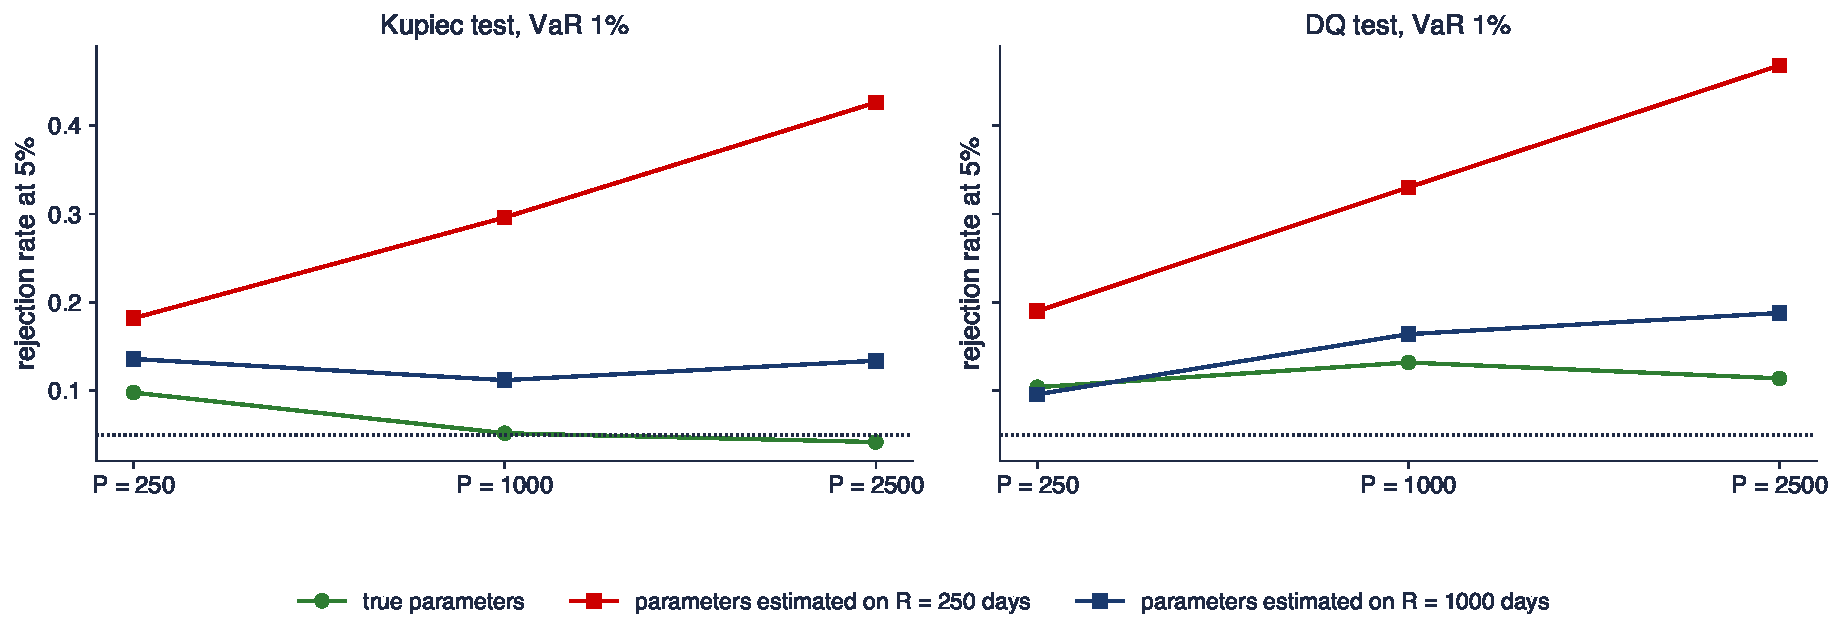
\includegraphics[width=0.97\textwidth,height=0.5\textheight,keepaspectratio]{ats_ch9_estrisk_mc.pdf}
\end{center}
\vspace{-0.25cm}
\begin{itemize}
    \item Date GARCH(1,1) ($\omega$ = 0,02, $\alpha$ = 0,08, $\beta$ = 0,90, distribuția Normală), modelul corect estimat prin QML pe $R$ zile, VaR 1\% pe următoarele $P$ zile; 500 de replicări; mărimea nominală 5\%
\end{itemize}
\quantlet{ATS\_ch9\_backtests}{\qlurl{ATS_ch9_backtests}}
\end{frame}

\begin{frame}{Interpretarea experimentului Monte Carlo}
\itemsize{\small}
\begin{itemize}
    \item Parametri cunoscuți: Kupiec respinge 10\%, 5\% și 4\% pentru $P$ = 250, 1000, 2500: aproape de 5\%, cu excepția cazului cu puține depășiri
    \item Estimat pe $R$ = 250: 18\%, 30\%, 43\%: un model corect este respins mai des cu cît testăm mai mult
    \item Cu $R$ = 1000 distorsiunea scade (13\% la $P$ = 2500); rata de depășire între replicări are abaterea standard 0{,}99 pp față de 0{,}29 pp
    \item DQ respinge prea des chiar cu parametri cunoscuți (10\%): depășirile rare fac aproximarea $\chi^2_6$ slabă
\end{itemize}
\end{frame}

\begin{frame}{Teste de calibrare pe active}
\itemsize{\footnotesize}
\begin{center}
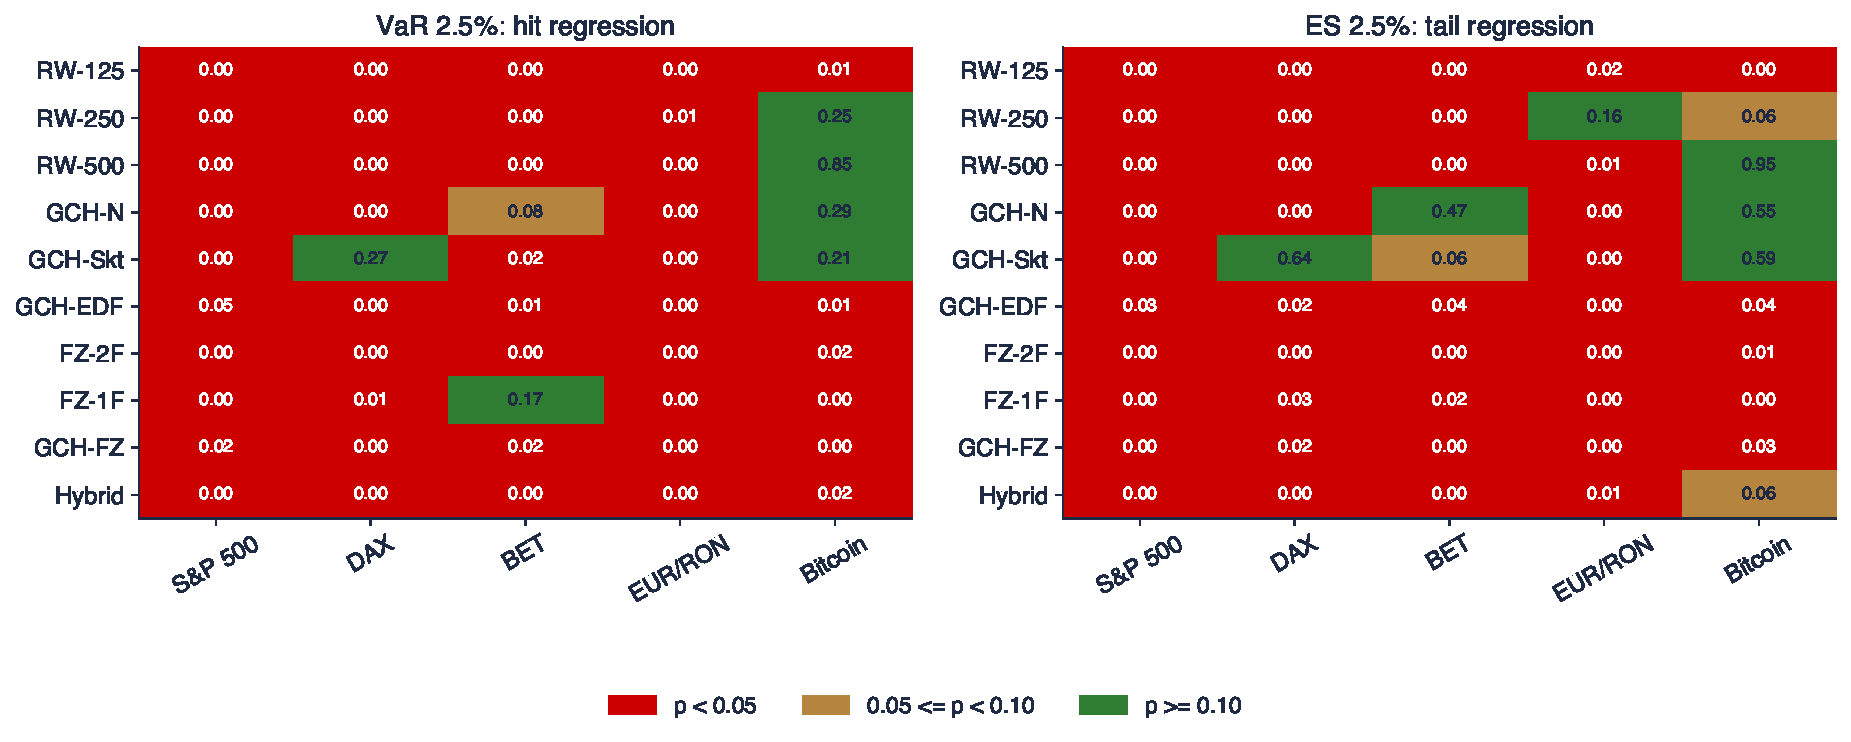
\includegraphics[width=0.97\textwidth,height=0.52\textheight,keepaspectratio]{ats_ch9_backtests.pdf}
\end{center}
\vspace{-0.25cm}
\begin{itemize}
    \item Regresiile de adecvare PZC pentru VaR și ES 2,5\%, zece modele, parametri estimați pe primii zece ani (cinci pentru Bitcoin) și păstrați ficși pînă la 18 septembrie 2026
\end{itemize}
\quantlet{ATS\_ch9\_backtests}{\qlurl{ATS_ch9_backtests}}
\end{frame}

\begin{frame}{Interpretarea testelor de calibrare}
\itemsize{\footnotesize}
\begin{itemize}
    \item Doar 4 din 50 de perechi activ--model trec ambele regresii la 10\%: pe 10--26 de ani cu parametri ficși, aproape orice model este necalibrat undeva
    \item Ratele de depășire S\&P 500 la 2,5\%: GAS-1F 3{,}2\%, GARCH-EDF 3{,}0\%, RW-250 3{,}3\%: nivelul derivă după deceniul de estimare
    \item EUR/RON: estimate pe 2005--2015 (criză și flotare), modelele GARCH supraestimează apoi riscul (GARCH-EDF 0{,}6\% depășiri): și necalibrarea în direcția prudentă este respinsă
    \item Bitcoin: istorie scurtă și coadă zgomotoasă, putere redusă; modelele simple trec (RW-500 2{,}5\%)
    \item Un backtest răspunde la „este calibrat?”; dacă un model respins este preferabil altuia este o întrebare de comparație
\end{itemize}
\end{frame}

\begin{frame}{Recapitulare: backtesting}
\itemsize{\small}
\begin{itemize}
    \item Backtesting-ul înseamnă teste de momente ale funcției de identificare cu instrumente alese
    \item Duratele surprind gruparea la orice distanță; testele ES cer mai mult decît ES, cu excepția testelor prin regresie
    \item Parametrii estimați cresc mărimea testelor; evaluările lungi, cu parametri ficși, resping aproape totul
\end{itemize}
\end{frame}


%=============================================================================
\section{Compararea prognozelor de risc}
%=============================================================================

\begin{frame}{De la backtesting la backtesting comparativ}
\itemsize{\small}
\begin{itemize}
    \item \refNZ: backtesting-ul tradițional testează $H_0$: „modelul băncii este calibrat”; backtesting-ul comparativ testează modelul băncii față de unul standard cu un scor consistent
    \begin{itemize}
        \item $H_0^-$: modelul intern cel puțin la fel de bun ca cel standard; $H_0^+$: cel mult la fel de bun; verde dacă $H_0^+$ se respinge, roșu dacă $H_0^-$ se respinge, galben altfel
    \end{itemize}
    \item Contează mulțimea de informații \refHE: o prognoză calibrată care folosește mai multă informație are un scor consistent așteptat mai mic
    \begin{itemize}
        \item deci o ordonare prin FZ0 răsplătește și calibrarea, și informația, ceea ce un backtest nu poate face
    \end{itemize}
    \item Instrumente din \atschlink{https://danpele.github.io/Advanced-Time-Series/RO/Cursuri/capitol1_evaluarea_prognozelor.pdf}{Capitolul 1}: DM cu varianță HAC \refDM, Giacomini--White pentru metode de prognoză estimate \refGW, MCS \refHLN
\end{itemize}
\end{frame}

\begin{frame}{Designul comparației}
\itemsize{\small}
\begin{itemize}
    \item Cele zece modele PZC, $\alpha$ = 2,5\%, pierderi FZ0 în afara eșantionului: S\&P 500 și DAX din 2000, BET din 2010, EUR/RON din iulie 2015, Bitcoin din 2020
    \item MCS de 90\% cu statistica $T_{\max}$, bootstrap pe blocuri mobile (blocuri de 10 zile pe toată perioada, 5 zile într-o perioadă de criză), 1000 de replicări
    \item Perioadele de criză fixate înainte de a vedea pierderile
    \begin{itemize}
        \item 2008: septembrie 2008 -- martie 2009; 2020: 19 februarie -- 30 iunie 2020; 2022: anul calendaristic; 2025: martie -- iunie 2025
        \item S\&P 500 în 2020: 93 de zile, dintre care 9 depășiri GAS-1F; în 2025: 83 de zile, 5 depășiri
    \end{itemize}
    \item O fereastră de criză conține puține zile din coadă: ne așteptăm la mulțimi MCS largi și la cîștigători instabili
\end{itemize}
\end{frame}

\begin{frame}{Pierderile în perioadele de criză}
\itemsize{\footnotesize}
\begin{center}
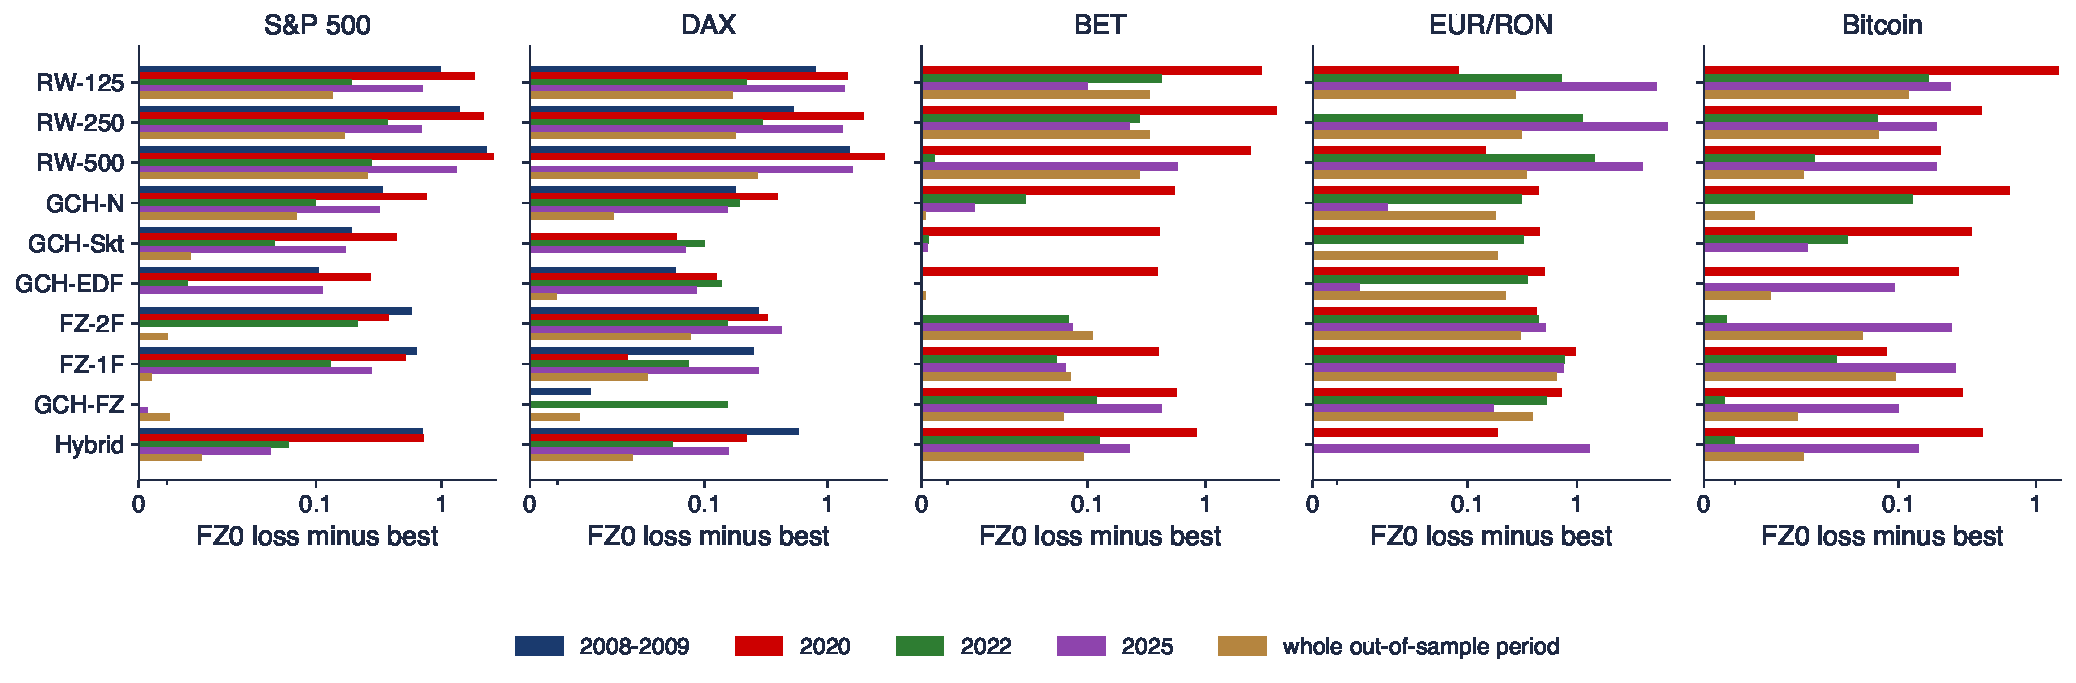
\includegraphics[width=0.97\textwidth,height=0.52\textheight,keepaspectratio]{ats_ch9_stress.pdf}
\end{center}
\vspace{-0.25cm}
\begin{itemize}
    \item Pierderea FZ0 medie a fiecărui model minus cea a celui mai bun model din aceeași perioadă (scară logaritmică simetrică); barele lipsesc cînd perioada nu este în afara eșantionului
\end{itemize}
\quantlet{ATS\_ch9\_comparison}{\qlurl{ATS_ch9_comparison}}
\end{frame}

\begin{frame}{Interpretarea pierderilor din perioadele de criză}
\itemsize{\footnotesize}
\begin{itemize}
    \item Cîștigătorii pe toată perioada: S\&P 500 GCH-EDF, DAX GCH-Skt, BET GCH-Skt, EUR/RON Hybrid, Bitcoin GCH-Skt
    \item În 2020 cîștigătorul se schimbă: S\&P 500 GCH-FZ, BET FZ-2F, Bitcoin FZ-2F; ferestrele mobile pierd cel mai mult în fiecare criză
    \item Crizele separă modelele cu un ordin de mărime mai mult decît anii calmi: o medie pe toată perioada este dominată de cîteva săptămîni
    \item Niciun model nu cîștigă fiecare criză; modelele semiparametrice sînt competitive, dar nu domină în afara eșantionului după 2016
\end{itemize}
\end{frame}

\begin{frame}{Mulțimi de încredere ale modelelor}
\itemsize{\footnotesize}
\begin{center}
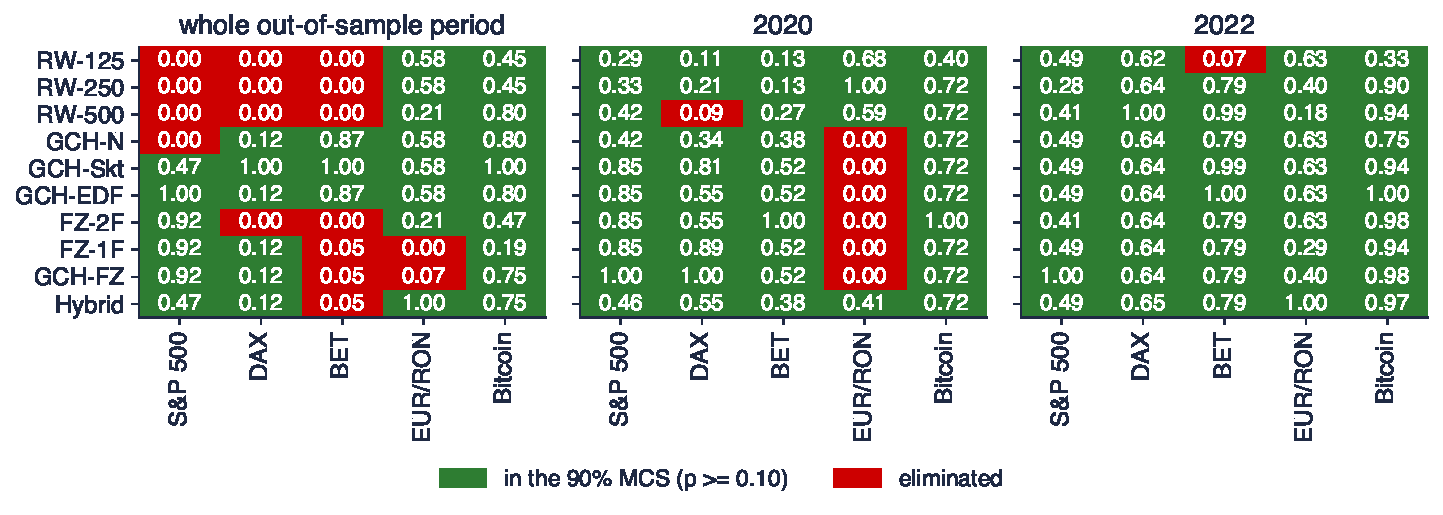
\includegraphics[width=0.97\textwidth,height=0.52\textheight,keepaspectratio]{ats_ch9_mcs.pdf}
\end{center}
\vspace{-0.25cm}
\begin{itemize}
    \item Valorile $p$ MCS (pierderea FZ0, $\alpha$ = 2,5\%); verde: în MCS de 90\%
\end{itemize}
\quantlet{ATS\_ch9\_comparison}{\qlurl{ATS_ch9_comparison}}
\end{frame}

\begin{frame}{Interpretarea mulțimilor MCS}
\itemsize{\small}
\begin{itemize}
    \item Toată perioada, mărimea MCS: S\&P 500 6, DAX 6, BET 3, EUR/RON 8, Bitcoin 10 din 10
    \item Ferestrele mobile sînt eliminate pe eșantioanele lungi de acțiuni; în 2020 și 2022 aproape totul rămîne (2020: 10 pe S\&P 500; 2022: 10)
    \item EUR/RON în 2020 este excepția: rămîn doar 4 modele, ferestrele mobile și Hybrid
    \item O mulțime MCS mare este un rezultat, nu un eșec: ferestrele de criză sînt prea scurte pentru a separa prognozele cozii
\end{itemize}
\end{frame}

\begin{frame}{Recapitulare: compararea}
\itemsize{\small}
\begin{itemize}
    \item Backtesting-ul comparativ pune sarcina probei pe model și răsplătește informația
    \item Ordonările se schimbă în crize; mediile pe toată perioada ascund acest lucru
    \item Raportați MCS, nu cîștigătorul
\end{itemize}
\end{frame}


%=============================================================================
\section{Orizontul: riscul pe mai multe perioade}
%=============================================================================

\begin{frame}{Limitele regulii rădăcinii pătrate a timpului}
\itemsize{\small}
\begin{itemize}
    \item $\mathrm{VaR}^{(h)} = \sqrt h\,\mathrm{VaR}^{(1)}$ este valabilă pentru randamente i.i.d.\ din distribuția Normală cu media zero (legi stabile: $h^{1/\gamma}$)
    \begin{itemize}
        \item cozi groase care nu sînt stabile: suma pe $h$ zile este mai apropiată de distribuția Normală decît randamentul zilnic, deci $\sqrt h$ supraestimează cuantila la orizonturi lungi \refDZ
    \end{itemize}
    \item Volatility clustering: $\mathrm{Var}_t(\sum_{k=1}^h y_{t+k}) = \sum_{k=0}^{h-1}\big[\bar\sigma^2 + (\alpha + \beta)^k(\sigma_{t+1}^2 - \bar\sigma^2)\big]$ pentru GARCH(1,1)
    \begin{itemize}
        \item în perioade calme $\sqrt h$ subestimează riscul, în crize îl supraestimează: revenirea volatilității la medie
    \end{itemize}
    \item Efectul de levier (GJR) face pierderile pe mai multe zile mai asimetrice decît cele zilnice: coada stîngă a sumei este mai groasă decît coada zilnică scalată
    \item Remedii: simularea distribuției pe $h$ zile (FHS) sau prognoza directă a cuantilei pe $h$ zile (regresie cuantilică pe randamentele pe $h$ zile)
\end{itemize}
\end{frame}

\begin{frame}{Prognozele pe mai multe zile și testarea lor}
\itemsize{\small}
\begin{itemize}
    \item FHS: GJR-GARCH(1,1) prin QML pe o fereastră mobilă de 2000 de zile (reestimat la fiecare 250 de zile); 2000 de traiectorii de 10 zile cu reziduuri standardizate extrase prin bootstrap \refBoll, \refGJR
    \item Backtesting pentru VaR pe 10 zile
    \begin{itemize}
        \item prognozele zilnice pe 10 zile se suprapun: depășirile sînt MA(9) chiar sub $H_0$; tratarea lor ca independente crește mărimea testului (\atschlink{https://danpele.github.io/Advanced-Time-Series/RO/Cursuri/capitol0_recapitulare_inferenta.pdf}{Capitolul 0}, observații suprapuse)
        \item variante: ferestre fără suprapunere (fiecare a zecea zi, puține depășiri) sau varianță HAC pentru depășirile suprapuse
    \end{itemize}
    \item Basel folosește orizonturi de 10 zile și orizonturi ajustate pentru lichiditate la ES (MAR33): problema orizontului este una de reglementare, nu academică
\end{itemize}
\end{frame}

\begin{frame}{VaR 1\% pe 10 zile față de regula rădăcinii pătrate}
\itemsize{\footnotesize}
\begin{center}
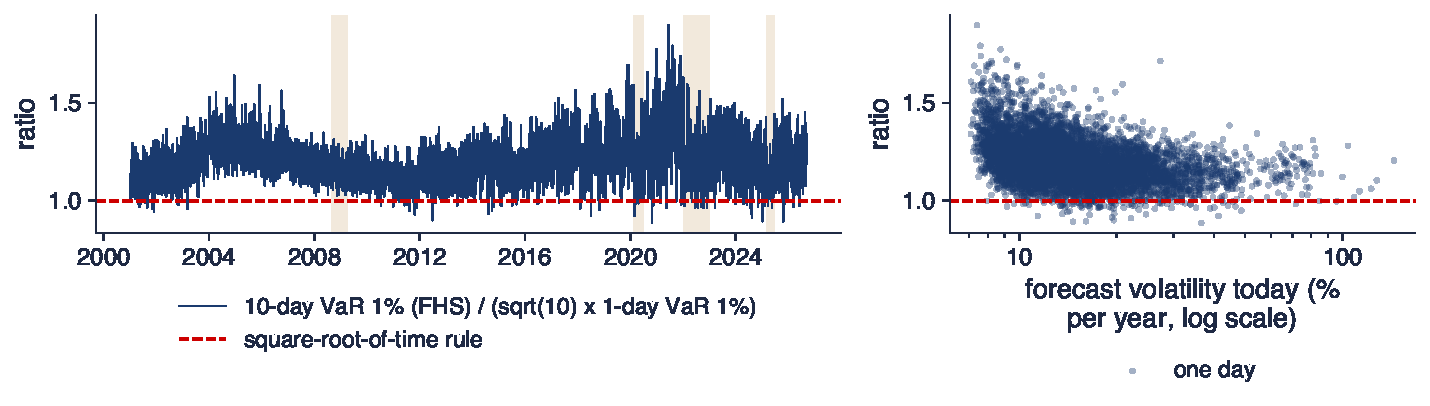
\includegraphics[width=0.97\textwidth,height=0.5\textheight,keepaspectratio]{ats_ch9_sqrt.pdf}
\end{center}
\vspace{-0.25cm}
\begin{itemize}
    \item S\&P 500, 2001--2026: raportul dintre VaR 1\% pe 10 zile prin FHS și $\sqrt{10}$ înmulțit cu VaR 1\% pe o zi al aceluiași model; dreapta: raportul în funcție de volatilitatea prognozată azi
\end{itemize}
\quantlet{ATS\_ch9\_horizon}{\qlurl{ATS_ch9_horizon}}
\end{frame}

\begin{frame}{Interpretarea raportului de orizont}
\itemsize{\small}
\begin{itemize}
    \item Raportul median 1{,}19, între 0{,}89 și 1{,}90: scalarea cu $\sqrt{10}$ subestimează de obicei VaR 1\% pe 10 zile pentru S\&P 500
    \item Zilele cu volatilitate scăzută: mediana 1{,}26; zilele cu volatilitate ridicată: 1{,}14: revenirea la medie împinge raportul spre 1 în crize
    \item Backtesting fără suprapunere (646 de ferestre, 6{,}5 depășiri așteptate): FHS 6, regula $\sqrt{10}$ 7; Kupiec $p$ 0{,}85 și 0{,}83
    \item Atît de puține depășiri nu le pot separa: erori de orizont de această mărime sînt invizibile pentru un backtest fără suprapunere
\end{itemize}
\end{frame}

\begin{frame}{Recapitulare: orizontul}
\itemsize{\small}
\begin{itemize}
    \item Regula rădăcinii pătrate cere randamente i.i.d.\ din distribuția Normală; volatility clustering, efectul de levier și cozile groase o contrazic în direcții opuse
    \item Simulați orizontul sau modelați-l direct; testați cu ferestre fără suprapunere sau cu varianțe HAC
    \item Testele pe mai multe zile au o putere foarte mică
\end{itemize}
\end{frame}


%=============================================================================
\section{Riscul de model și riscul de estimare}
%=============================================================================

\begin{frame}{Riscul de model al modelelor de risc}
\itemsize{\small}
\begin{itemize}
    \item \refDJVZ: \textbf{raportul de risc} $\mathrm{RR}_t = \max_m\mathrm{VaR}_{m,t}/\min_m\mathrm{VaR}_{m,t}$ între modele standard: dezacordul la care trebuie să se aștepte un supraveghetor
    \begin{itemize}
        \item ei găsesc raportul cel mai mare tocmai în crize, cînd cifrele de risc contează cel mai mult
    \end{itemize}
    \item \refBDKM: \textbf{risk models-at-risk}: cuantificăm riscul de model al unei prognoze VaR și ajustăm prognoza pentru erorile de estimare și de specificare
    \item \refKR: ES are mai mult risc de model decît VaR la niveluri comparabile: extrapolează mai departe în coadă
    \item Cele șase modele ale noastre, ferestre mobile de 1000 de zile: simulare istorică, distribuția Normală cu volatilitatea ferestrei, EWMA ($\lambda$ = 0,94), GARCH-N, GARCH-t, FHS
\end{itemize}
\end{frame}

\begin{frame}{Cît de mult diferă modelele standard?}
\itemsize{\footnotesize}
\begin{center}
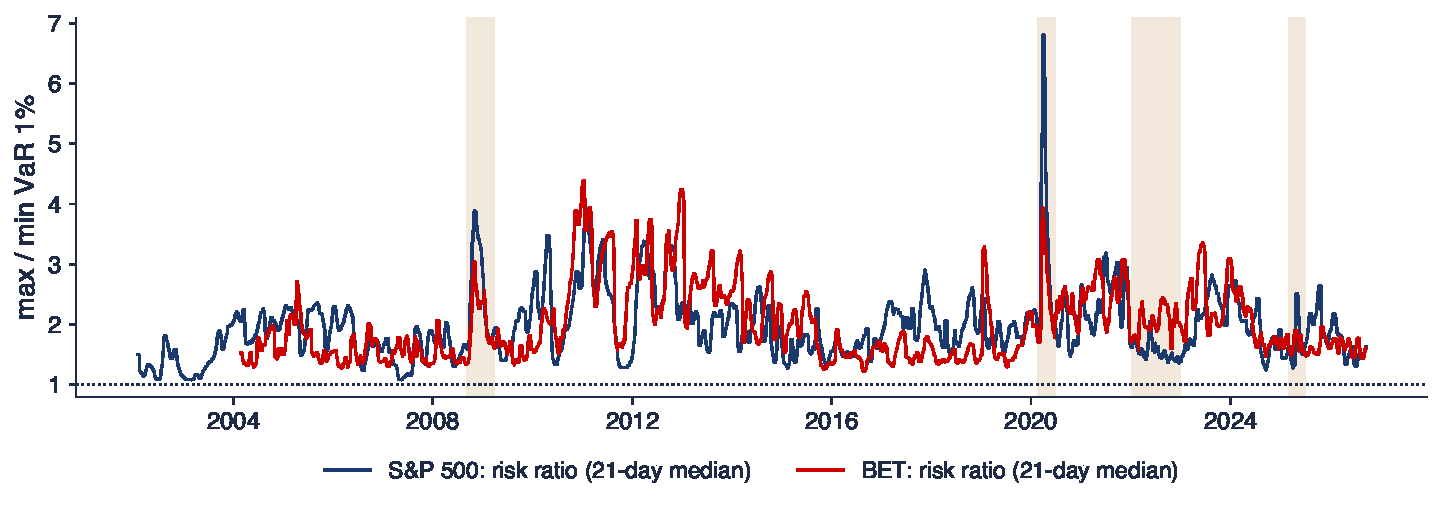
\includegraphics[width=0.97\textwidth,height=0.5\textheight,keepaspectratio]{ats_ch9_riskratio.pdf}
\end{center}
\vspace{-0.25cm}
\begin{itemize}
    \item Raportul de risc al celor șase prognoze VaR 1\%, mediana mobilă pe 21 de zile, S\&P 500 și BET, 2002--2026 (BET din 2004); zonele colorate: perioadele de criză
\end{itemize}
\quantlet{ATS\_ch9\_modelrisk}{\qlurl{ATS_ch9_modelrisk}}
\end{frame}

\begin{frame}{Interpretarea raportului de risc}
\itemsize{\footnotesize}
\begin{itemize}
    \item Raportul de risc median 1{,}9 (S\&P 500) și 1{,}8 (BET); percentila 90 2{,}7 și 3{,}0; maximul 10{,}5 la 17 martie 2020
    \item Primăvara 2020: mediana 2{,}9 (S\&P 500), 2{,}5 (BET): simularea istorică lentă și EWMA rapid diverg cel mai mult după un salt
    \item HS este cel mai prudent model în 73\% din zilele S\&P 500, EWMA cel mai puțin prudent în 53\%
    \item Ratele de depășire VaR 1\% (S\&P 500): HS 1{,}4\%, GARCH-N 2{,}2\%, GARCH-t 1{,}4\%, FHS 1{,}3\%: dezacordul nu este zgomot, modelele cu distribuția Normală greșesc
\end{itemize}
\end{frame}

\begin{frame}{Riscul de estimare în prognozele cozii}
\itemsize{\small}
\begin{itemize}
    \item \refGS: pentru VaR și ES din GARCH, $\sqrt T(\widehat{\mathrm{ES}}_t - \mathrm{ES}_t)$ este asimptotic normal; varianța are o parte din volatilitate și una din forma cozii
    \item Bootstrap \refCG: reestimăm modelul pe traiectorii simulate și recalculăm prognoza \textbf{condiționat de istoria observată}
    \begin{itemize}
        \item algoritm: estimăm GARCH-t pe 2000 de zile; simulăm 150 de traiectorii de 2000 de zile din modelul estimat; reestimăm pe fiecare; filtrăm randamentele observate cu fiecare $\hat\theta^*$; ES$^*$ pentru ziua următoare
        \item intervalul de 90\%: cuantilele de 5\% și 95\% ale ES$^*$
    \end{itemize}
    \item Intervalul măsoară doar incertitudinea parametrilor: este condiționat de corectitudinea modelului, deci este o limită inferioară a incertitudinii totale
\end{itemize}
\end{frame}

\begin{frame}{O prognoză ES cu eroarea ei de estimare}
\itemsize{\footnotesize}
\begin{center}
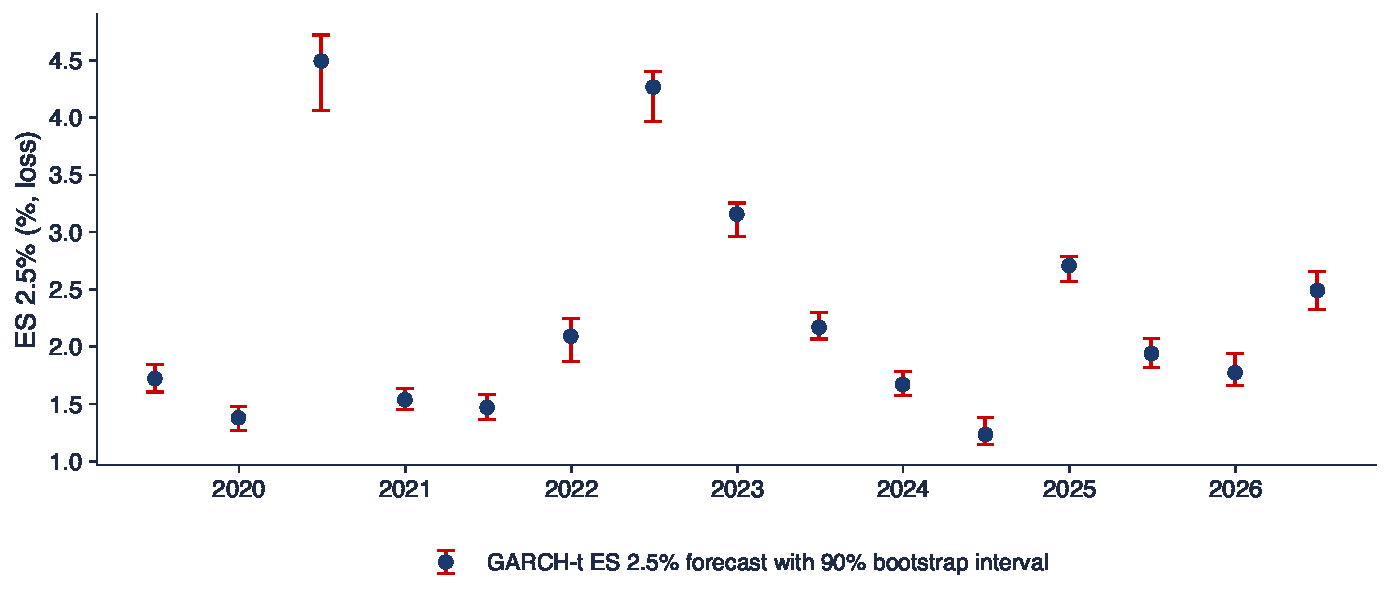
\includegraphics[width=0.97\textwidth,height=0.5\textheight,keepaspectratio]{ats_ch9_es_ci.pdf}
\end{center}
\vspace{-0.25cm}
\begin{itemize}
    \item S\&P 500, ES 2,5\% GARCH-t pentru ziua următoare la sfîrșitul fiecărui semestru 2019--2026, cu intervale bootstrap parametric de 90\% (cîte 150 de reestimări)
\end{itemize}
\quantlet{ATS\_ch9\_modelrisk}{\qlurl{ATS_ch9_modelrisk}}
\end{frame}

\begin{frame}{Interpretarea erorii de estimare}
\itemsize{\small}
\begin{itemize}
    \item Lățimea intervalului raportată la prognoză: mediana 13\%, între 8\% și 19\%
    \item Iunie 2020: ES 4{,}49\% cu intervalul [4{,}06; 4{,}72]: două mii de zile de date lasă totuși o bandă de cîteva zecimi de procent
    \item Riscul de estimare este mic față de riscul de model (rapoarte de risc în jur de 2): alegerea modelului contează mai mult decît precizia lui
    \item Regulile de capital care multiplică o prognoză punctuală le ignoră pe amîndouă: raportarea intervalului este minimul onest
\end{itemize}
\end{frame}

\begin{frame}{Recapitulare: riscul de model și de estimare}
\itemsize{\small}
\begin{itemize}
    \item Modelele standard diferă cu un factor de circa doi, mai mult în crize
    \item Intervalele bootstrap pentru ES sînt înguste față de acest dezacord
    \item Raportați ambele: prognoza, intervalul ei și dispersia între modele
\end{itemize}
\end{frame}


%=============================================================================
\section{Extreme sub dependență și calibrare conformală}
%=============================================================================

\begin{frame}{Extremele seriilor dependente}
\itemsize{\small}
\begin{itemize}
    \item Pentru o serie staționară, $\Pr(\max_{t \le n} X_t \le u_n) \approx F(u_n)^{n\theta}$, $\theta \in (0, 1]$ fiind \textbf{indicele extremal} \refEKM
    \begin{itemize}
        \item $1/\theta$ = mărimea medie a unui grup de depășiri; $\theta = 1$: extremele nu se grupează
    \end{itemize}
    \item Estimatorul pe intervale \refFS: din distanțele $T_i$ dintre depășiri, $\hat\theta = \min\Big(1, \dfrac{2\big(\sum(T_i - 1)\big)^2}{(N - 1)\sum(T_i - 1)(T_i - 2)}\Big)$ (cînd $\max T_i > 2$)
    \item \refMF: estimăm GARCH, aplicăm EVT reziduurilor standardizate; metoda funcționează dacă filtrarea elimină gruparea ($\theta$ aproape de 1 după filtrare)
\end{itemize}
\end{frame}

\begin{frame}{Indicele extremal înainte și după filtrare}
\itemsize{\footnotesize}
\begin{center}
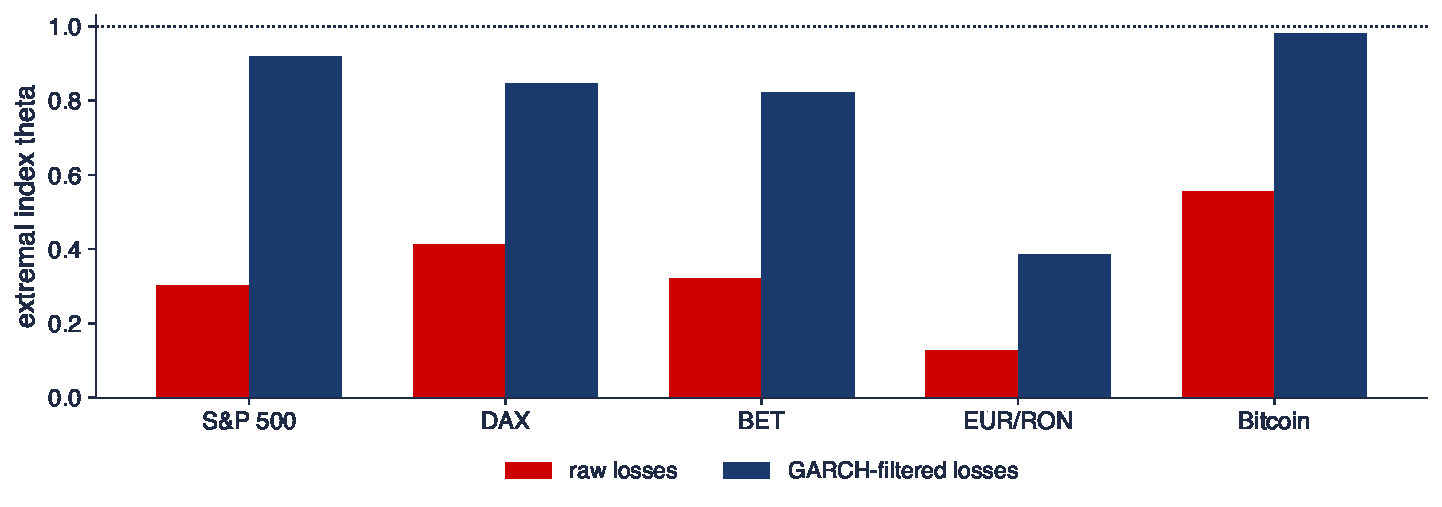
\includegraphics[width=0.97\textwidth,height=0.48\textheight,keepaspectratio]{ats_ch9_extremal.pdf}
\end{center}
\vspace{-0.25cm}
\begin{itemize}
    \item Depășiri ale pierderilor zilnice peste cuantila lor de 95\%, eșantioanele întregi; pierderi brute și pierderi standardizate prin GARCH (parametri ARMA-GARCH din eșantion)
\end{itemize}
\quantlet{ATS\_ch9\_extremes}{\qlurl{ATS_ch9_extremes}}
\end{frame}

\begin{frame}{Interpretarea indicelui extremal}
\itemsize{\small}
\begin{itemize}
    \item Pierderi brute: $\hat\theta$ = 0{,}30 (S\&P 500), 0{,}32 (BET), 0{,}13 (EUR/RON): extremele vin în grupuri de două pînă la opt zile
    \item După filtrare: 0{,}92; 0{,}85; 0{,}98 pentru S\&P 500, DAX și Bitcoin: GARCH elimină cea mai mare parte a grupării, cum presupun McNeil și Frey
    \item EUR/RON rămîne grupat (0{,}39) și BET parțial (0{,}82): un curs administrat și o piață mică au o dependență pe care GARCH nu o surprinde
    \item Cu parametri ficși din eșantion, filtrul este imperfect după perioada de estimare: o parte din gruparea rămasă este derivă
\end{itemize}
\end{frame}

\begin{frame}{Calibrarea conformală a VaR}
\itemsize{\small}
\begin{itemize}
    \item Cuantilele conformale split garantează acoperirea sub interschimbabilitate (\atschlink{https://danpele.github.io/Advanced-Time-Series/RO/Cursuri/capitol13_foundation_models_conformal.pdf}{Capitolul 13}); randamentele nu sînt interschimbabile, deci garanția nu mai este valabilă
    \item \textbf{Inferența conformală adaptivă} \refGC: prognozăm la nivelul $\alpha_t$ și actualizăm $\alpha_{t+1} = \alpha_t + \gamma(\alpha - \mathrm{err}_t)$, $\mathrm{err}_t = \mathbf 1\{y_t < q_t(\alpha_t)\}$
    \begin{itemize}
        \item garanție deterministă: $\big|T^{-1}\sum_t\mathrm{err}_t - \alpha\big| \le \dfrac{\max(\alpha_1, 1 - \alpha_1) + \gamma}{\gamma T}$ pentru \textbf{orice} șir de randamente
        \item doar frecvența pe termen lung: nici calibrare condiționată, nici vreo afirmație despre ES
    \end{itemize}
    \item Lectură suplimentară: recalibrarea conformală a cuantilelor extreme sub dependență \refCO
\end{itemize}
\end{frame}

\begin{frame}{Corecția conformală adaptivă a VaR 1\%}
\itemsize{\footnotesize}
\begin{center}
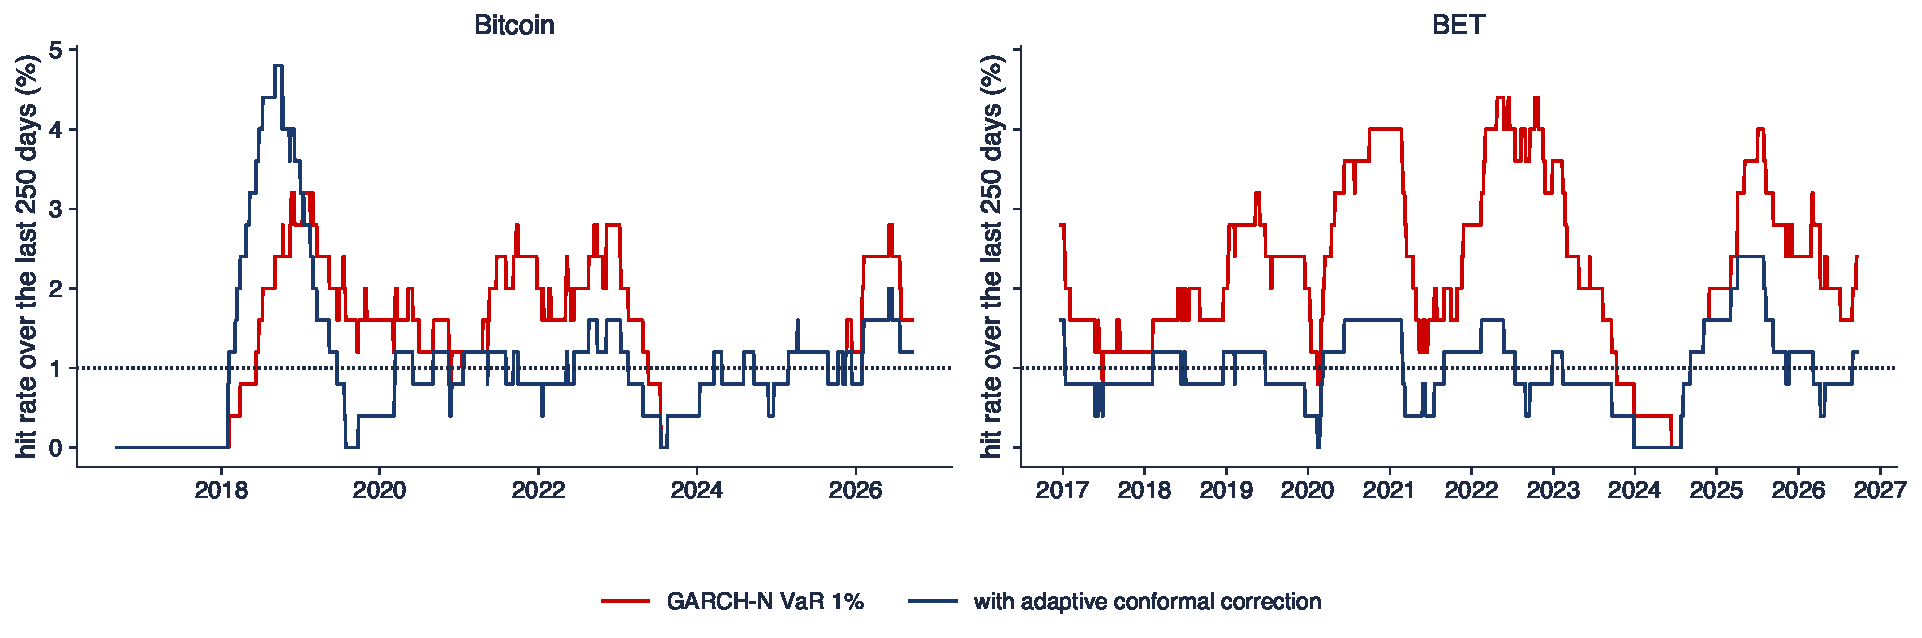
\includegraphics[width=0.97\textwidth,height=0.5\textheight,keepaspectratio]{ats_ch9_conformal.pdf}
\end{center}
\vspace{-0.25cm}
\begin{itemize}
    \item VaR 1\% GARCH-N (fereastră mobilă de 1000 de zile, reestimat la fiecare 250 de zile) din 2016 și corecția ACI cu $\gamma$ = 0,005; ratele de depășire pe 250 de zile
\end{itemize}
\quantlet{ATS\_ch9\_conformal}{\qlurl{ATS_ch9_conformal}}
\end{frame}

\begin{frame}{Interpretarea corecției conformale}
\itemsize{\small}
\begin{itemize}
    \item BET: GARCH-N are depășiri în 2{,}36\% din 2\,675 de zile (Kupiec $p$ $<$0{,}001); cu ACI 1{,}08\% ($p$ = 0{,}666), acoperire condiționată $p$ = 0{,}662
    \item Bitcoin: de la 1{,}28\% la 1{,}02\%; rata mobilă nu se netezește: maximul crește de la 3{,}2\% la 4{,}8\% după o supracorecție
    \item ACI corectează frecvența, nu dinamica: nivelul adaptat poate coborî sub zero (VaR devine atunci infinit) după un șir de zile liniștite
    \item Un înveliș util pentru numărătoarea supraveghetorului; pentru DQ și pentru ES este în continuare nevoie de un model calibrat
\end{itemize}
\end{frame}

\begin{frame}{Recapitulare: extreme și calibrare conformală}
\itemsize{\small}
\begin{itemize}
    \item Extremele se grupează; filtrarea elimină cea mai mare parte a grupării pe piețele lichide, nu și pentru cursurile administrate
    \item ACI garantează frecvența pe termen lung a depășirilor pentru orice date, nimic mai mult
    \item Ambele sînt corecții ale unui model, nu înlocuitori ai lui
\end{itemize}
\end{frame}


%=============================================================================
\section{AI în descoperirea științifică}
%=============================================================================

\begin{frame}{O întrebare deschisă}
\itemsize{\small}
\begin{itemize}
    \item Bat modelele semiparametrice (VaR, ES) modelele de tip poziție--scală în afara eșantionului atunci cînd estimarea se repetă și este avantajul concentrat în crize?
    \begin{itemize}
        \item formal: $H_0$: pierdere FZ0 așteptată egală pentru GAS-1F și GARCH-EDF cu reestimare mobilă, pe active, perioade și niveluri preînregistrate
        \item infirmată de o statistică GW semnificativă în ferestrele de criză preînregistrate, robustă pentru $\alpha$ = 1\%, 2,5\%, 5\%
    \end{itemize}
    \item De ce contează: Basel cere modele ES; evidența PZC provine din parametri ficși și patru indici
    \begin{itemize}
        \item literatura de pornire: \refPZC, \refTayB, \refNZ, \refDB
    \end{itemize}
\end{itemize}
\end{frame}

\begin{frame}{Bucla de cercetare cu un asistent AI}
\itemsize{\footnotesize}
\begin{itemize}
    \item Un asistent AI (un LLM precum Claude, ChatGPT, Gemini sau Copilot) accelerează fiecare etapă; Semantic Scholar și Elicit ajută la literatură
    \begin{itemize}
        \item \textbf{literatura}: \aiprompt{Listează articole recenzate din 2017 încoace care compară modele dinamice pentru ES în afara eșantionului cu pierderi FZ; dă DOI-urile.} Apoi verificați fiecare DOI pe Crossref
        \item \textbf{ipoteza}: \aiprompt{În ce procese generatoare ar trebui ca un model GAS cu un factor să bată GARCH cu inovații empirice pentru ES 2,5\%?}
        \item \textbf{cod și replicare}: cereți recursia GAS-1F, apoi reproduceți întîi o cifră publicată (PZC, Tabelul 8: 0{,}853)
        \item \textbf{critica}: \aiprompt{Joacă rolul unui recenzent ostil: enumeră felurile în care o ordonare FZ0 poate fi un artefact al eșantionului, al nivelului sau al valorilor de pornire.}
    \end{itemize}
    \item Raportul: ce s-a cerut, ce s-a păstrat, ce s-a respins (AI\_USE.md, AI\_ERRORS.md)
\end{itemize}
\end{frame}

\begin{frame}{Verificări necesare}
\itemsize{\small}
\begin{itemize}
    \item Fiecare referință există și spune ce se afirmă (DOI-ul funcționează, titlul coincide, rezultatul se află în lucrare)
    \item Pierderea este consistentă pentru țintă: fără „eroarea medie a ES”, fără MSE pentru prognozele VaR
    \item Convenția este corectă: VaR 1\% este cuantila de 1\% a randamentelor cu semn schimbat, niciodată „VaR 99\%”; semnele lui $v$ și $e$ sînt consecvente
    \item Prognozele folosesc doar informația disponibilă la $t - 1$; fereastra de estimare și schema de reestimare sînt precizate
    \item Ordonările se raportează cu incertitudinea DM sau MCS și se verifică pe o diagramă Murphy
\end{itemize}
\end{frame}

\begin{frame}{Mini studiu de caz: există un cel mai bun model ES?}
\itemsize{\footnotesize}
\begin{center}
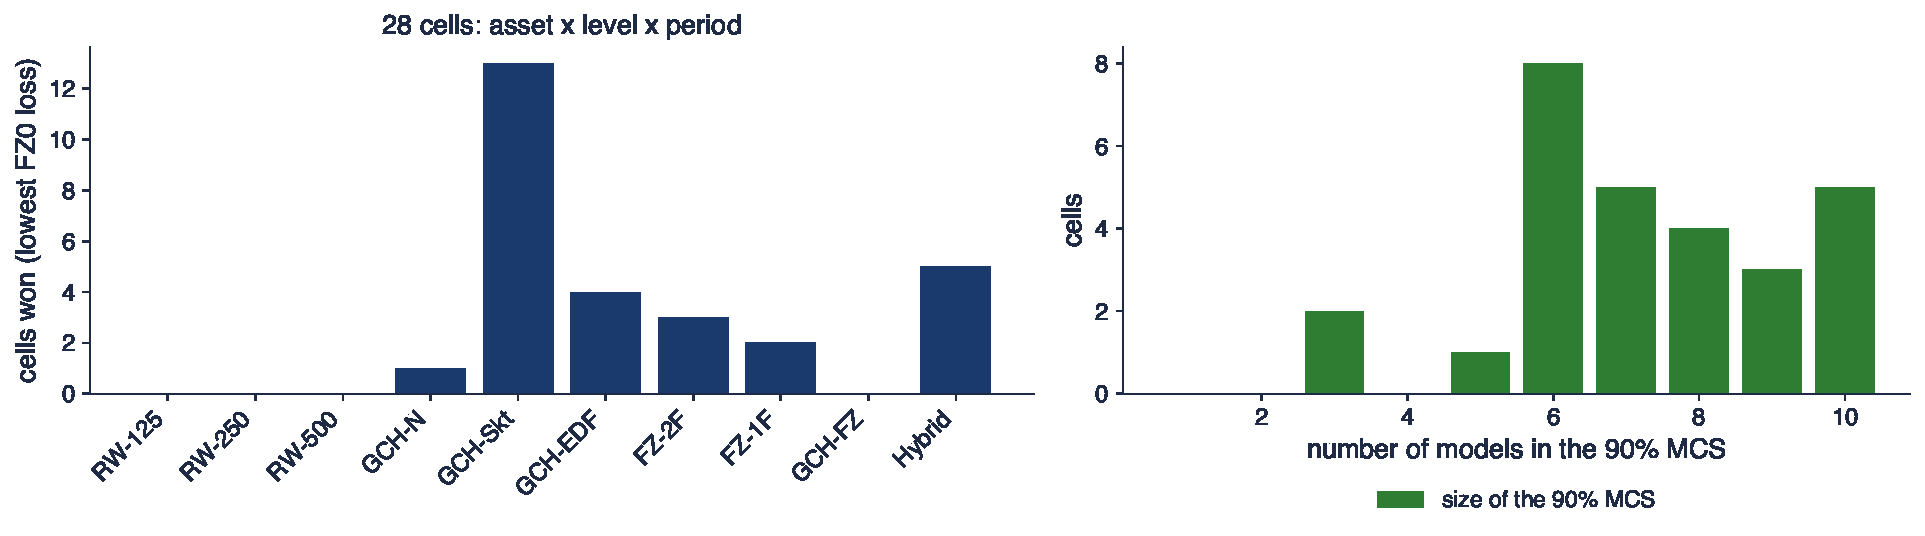
\includegraphics[width=0.97\textwidth,height=0.44\textheight,keepaspectratio]{ats_ch9_ai_case.pdf}
\end{center}
\vspace{-0.25cm}
\begin{itemize}
    \item 28 de celule: cinci active $\times$ două niveluri (2,5\%, 5\%) $\times$ pînă la trei perioade (toată, înainte de 2020, din 2020); stînga: modelul cu cea mai mică pierdere FZ0; dreapta: mărimea MCS de 90\%
    \item 6 cîștigători diferiți; GARCH-Skt cîștigă 13 celule, GAS-1F 2; mărimea MCS între 3 și 10, mediana 7; GAS-1F este în MCS în 22 de celule: un rezumat AI care numește „cel mai bun model ES” greșește
\end{itemize}
\quantlet{ATS\_ch9\_comparison}{\qlurl{ATS_ch9_comparison}}
\end{frame}

\begin{frame}{Idee de proiect}
\itemsize{\small}
\begin{itemize}
    \item \textbf{Modele ES pentru piețele din Europa Centrală și de Est cu reestimare mobilă}: întîi replicare, apoi extindere
    \begin{itemize}
        \item replicați: Tabelele 8 și S5 din PZC pentru S\&P 500 (GAS-1F 0{,}853 și 1{,}032) și designul EM cu VaR 1\%
        \item extindeți: BET, WIG20, BUX, PX și EUR/RON; reestimare mobilă; regresii comune (VaR, ES) cu VIX și dobînda BNR; ACI ca înveliș
        \item preînregistrați: eșantioanele, nivelurile, modelele, ferestrele, perioadele de criză și designul MCS
    \end{itemize}
    \item Livrabilele urmează regulile cursului: repository, raport, AI\_USE.md, AI\_ERRORS.md, susținere orală
\end{itemize}
\end{frame}


%=============================================================================
\section{Încheiere}
%=============================================================================

\begin{frame}{Idei de reținut}
\itemsize{\small}
\begin{itemize}
    \item O prognoză de risc este o prognoză punctuală a unei funcționale; judecați-o cu o pierdere consistentă pentru acea funcțională
    \item VaR este elicitabil, ES doar împreună cu VaR; FZ0 este alegerea independentă de scală pentru serii de timp
    \item Modelele CAViaR și GAS-FZ estimează direct coada; ordonările publicate se replică, testele publicate nu
    \item Backtesting-ul înseamnă teste de momente cu risc de estimare; comparațiile cer DM, MCS și diagrame Murphy
    \item Riscul de orizont, de model și de estimare sînt mai mari decît sugerează majoritatea rezultatelor raportate
\end{itemize}
\end{frame}

\begin{frame}{Autoevaluare}
\itemsize{\small}
\begin{columns}[T]
\begin{column}{0.56\textwidth}
\begin{block}{Întrebări}
\begin{itemize}
    \item De ce exclude o mulțime de nivel neconvexă existența unei pierderi strict consistente pentru ES?
    \item Ce alegere a lui $(G_1, G_2)$ dă FZ0 și ce aduce omogenitatea de grad zero?
    \item De ce este testul DQ cu regresorul VaR mai puternic decît testul lui Christoffersen?
    \item De ce crește o fereastră fixă de estimare mărimea testului Kupiec?
    \item Cînd supraestimează scalarea cu $\sqrt{10}$ VaR pe 10 zile?
\end{itemize}
\end{block}
\end{column}
\begin{column}{0.40\textwidth}
\begin{block}{Urmează: \atschlink{https://danpele.github.io/Advanced-Time-Series/RO/Cursuri/capitol10_memorie_lunga_rough_volatility.pdf}{Capitolul 10}}
\begin{itemize}
    \item Memorie lungă și rough volatility
    \item ARFIMA, cointegrare fracționară, rough volatility
\end{itemize}
\end{block}
\end{column}
\end{columns}
\end{frame}


%=============================================================================
\section{Anexă}
%=============================================================================

\begin{frame}{Anexă: consistența scorurilor GPL pentru cuantile}
\hypertarget{atsapp1}{}\atsappback{atssrc1}{Înapoi}
\itemsize{\small}
\begin{itemize}
    \item $\E_F S(x, Y) = \int_{-\infty}^x(1 - \alpha)(G(x) - G(y))\,dF(y) + \int_x^\infty \alpha(G(y) - G(x))\,dF(y)$
    \item Derivăm (Leibniz; termenii de frontieră se anulează): $\dfrac{d}{dx}\E_F S(x, Y) = G'(x)\big[(1 - \alpha)F(x) - \alpha(1 - F(x))\big] = G'(x)(F(x) - \alpha)$
    \item $G' \ge 0$: derivata este $\le 0$ pentru $x < q_\alpha$ și $\ge 0$ pentru $x > q_\alpha$, deci $q_\alpha$ minimizează; strict dacă $G$ este strict crescătoare și $F$ are o singură cuantilă de nivel $\alpha$
    \item Același calcul cu $G(x) = x$ este condiția de ordinul întîi a regresiei cuantilice
\end{itemize}
\end{frame}

\begin{frame}{Anexă: FZ0, consistență și omogenitate}
\hypertarget{atsapp2}{}\atsappback{atssrc1}{Înapoi}
\itemsize{\small}
\begin{itemize}
    \item Fixăm $e$; în $v$, FZ0 este $-\frac{1}{\alpha e}\big[\mathbf 1\{y \le v\}(v - y) - \alpha v\big]$ plus termeni fără $v$: deoarece $-1/(\alpha e) > 0$, un multiplu pozitiv al pierderii pinball, minimizat în $q_\alpha$
    \item La $v = q_\alpha$: $\E\,L = \dfrac{c}{e} + \ln(-e) - 1$ cu $c = v - \frac1\alpha\E[\mathbf 1\{Y \le v\}(v - Y)] = \E[Y \mid Y \le q_\alpha] = -\mathrm{ES}_\alpha$; derivata $-c/e^2 + 1/e$ se anulează în $e = c$
    \item Omogenitate: înlocuind $(y, v, e)$ cu $(sy, sv, se)$, $s > 0$, FZ0 se schimbă doar cu $\ln s$, la fel pentru orice prognoză: diferențele de pierdere nu depind de scală
    \item Minimizarea comună în $(v, e)$ cu $e \le v < 0$ dă deci $(q_\alpha, -\mathrm{ES}_\alpha)$
\end{itemize}
\end{frame}


%=============================================================================
\section{Bibliografie}
%=============================================================================

\begin{frame}{Bibliografie (1/4)}
\itemsize{\tiny}
\begin{itemize}
    \item Acerbi, C., \& Székely, B. (2014). Backtesting expected shortfall. \textit{Risk}, December 2014 (MSCI working paper). \href{https://www.msci.com/documents/10199/22aa9922-f874-4060-b77a-0f0e267a489b}{msci.com}
    \item Acerbi, C., \& Tasche, D. (2002). On the coherence of expected shortfall. \textit{Journal of Banking \& Finance}, 26(7), 1487--1503. \href{https://doi.org/10.1016/S0378-4266(02)00283-2}{doi:10.1016/S0378-4266(02)00283-2}
    \item Artzner, P., Delbaen, F., Eber, J.-M., \& Heath, D. (1999). Coherent measures of risk. \textit{Mathematical Finance}, 9(3), 203--228. \href{https://doi.org/10.1111/1467-9965.00068}{doi:10.1111/1467-9965.00068}
    \item Basel Committee on Banking Supervision (2019). \textit{MAR33: Internal models approach, capital requirements calculation}. Basel Framework, Bank for International Settlements. \href{https://www.bis.org/basel_framework/chapter/MAR/33.htm}{bis.org}
    \item Basel Committee on Banking Supervision (1996). \textit{Supervisory framework for the use of ``backtesting in conjunction with the internal models approach to market risk capital requirements}. Bank for International Settlements. \href{https://www.bis.org/publ/bcbs22.htm}{bis.org}
    \item Bayer, S., \& Dimitriadis, T. (2022). Regression-based expected shortfall backtesting. \textit{Journal of Financial Econometrics}, 20(3), 437--471. \href{https://doi.org/10.1093/jjfinec/nbaa013}{doi:10.1093/jjfinec/nbaa013}
    \item Bollerslev, T. (1986). Generalized autoregressive conditional heteroskedasticity. \textit{Journal of Econometrics}, 31(3), 307--327. \href{https://doi.org/10.1016/0304-4076(86)90063-1}{doi:10.1016/0304-4076(86)90063-1}
    \item Boucher, C. M., Daníelsson, J., Kouontchou, P. S., \& Maillet, B. B. (2014). Risk models-at-risk. \textit{Journal of Banking \& Finance}, 44, 72--92. \href{https://doi.org/10.1016/j.jbankfin.2014.03.019}{doi:10.1016/j.jbankfin.2014.03.019}
    \item Christoffersen, P. F. (1998). Evaluating interval forecasts. \textit{International Economic Review}, 39(4), 841--862. \href{https://doi.org/10.2307/2527341}{doi:10.2307/2527341}
    \item Christoffersen, P., \& Gonçalves, S. (2005). Estimation risk in financial risk management. \textit{The Journal of Risk}, 7(3), 1--28. \href{https://doi.org/10.21314/JOR.2005.112}{doi:10.21314/JOR.2005.112}
    \item Christoffersen, P., \& Pelletier, D. (2004). Backtesting value-at-risk: A duration-based approach. \textit{Journal of Financial Econometrics}, 2(1), 84--108. \href{https://doi.org/10.1093/jjfinec/nbh004}{doi:10.1093/jjfinec/nbh004}
    \item Creal, D., Koopman, S. J., \& Lucas, A. (2013). Generalized autoregressive score models with applications. \textit{Journal of Applied Econometrics}, 28(5), 777--795. \href{https://doi.org/10.1002/jae.1279}{doi:10.1002/jae.1279}
    \item Daníelsson, J., \& Zigrand, J.-P. (2006). On time-scaling of risk and the square-root-of-time rule. \textit{Journal of Banking \& Finance}, 30(10), 2701--2713. \href{https://doi.org/10.1016/j.jbankfin.2005.10.002}{doi:10.1016/j.jbankfin.2005.10.002}
\end{itemize}
\end{frame}

\begin{frame}{Bibliografie (2/4)}
\itemsize{\tiny}
\begin{itemize}
    \item Danielsson, J., James, K. R., Valenzuela, M., \& Zer, I. (2016). Model risk of risk models. \textit{Journal of Financial Stability}, 23, 79--91. \href{https://doi.org/10.1016/j.jfs.2016.02.002}{doi:10.1016/j.jfs.2016.02.002}
    \item Diebold, F. X., \& Mariano, R. S. (1995). Comparing predictive accuracy. \textit{Journal of Business \& Economic Statistics}, 13(3), 253--263. \href{https://doi.org/10.1080/07350015.1995.10524599}{doi:10.1080/07350015.1995.10524599}
    \item Dimitriadis, T., \& Bayer, S. (2019). A joint quantile and expected shortfall regression framework. \textit{Electronic Journal of Statistics}, 13(1), 1823--1871. \href{https://doi.org/10.1214/19-EJS1560}{doi:10.1214/19-EJS1560}
    \item Du, Z., \& Escanciano, J. C. (2017). Backtesting expected shortfall: Accounting for tail risk. \textit{Management Science}, 63(4), 940--958. \href{https://doi.org/10.1287/mnsc.2015.2342}{doi:10.1287/mnsc.2015.2342}
    \item Ehm, W., Gneiting, T., Jordan, A., \& Krüger, F. (2016). Of quantiles and expectiles: Consistent scoring functions, Choquet representations and forecast rankings. \textit{Journal of the Royal Statistical Society: Series B}, 78(3), 505--562. \href{https://doi.org/10.1111/rssb.12154}{doi:10.1111/rssb.12154}
    \item Embrechts, P., Klüppelberg, C., \& Mikosch, T. (1997). \textit{Modelling Extremal Events for Insurance and Finance}. Springer. \href{https://doi.org/10.1007/978-3-642-33483-2}{doi:10.1007/978-3-642-33483-2}
    \item Engle, R. F., \& Manganelli, S. (2004). CAViaR: Conditional autoregressive value at risk by regression quantiles. \textit{Journal of Business \& Economic Statistics}, 22(4), 367--381. \href{https://doi.org/10.1198/073500104000000370}{doi:10.1198/073500104000000370}
    \item Escanciano, J. C., \& Olmo, J. (2010). Backtesting parametric value-at-risk with estimation risk. \textit{Journal of Business \& Economic Statistics}, 28(1), 36--51. \href{https://doi.org/10.1198/jbes.2009.07063}{doi:10.1198/jbes.2009.07063}
    \item Ferro, C. A. T., \& Segers, J. (2003). Inference for clusters of extreme values. \textit{Journal of the Royal Statistical Society: Series B}, 65(2), 545--556. \href{https://doi.org/10.1111/1467-9868.00401}{doi:10.1111/1467-9868.00401}
    \item Fissler, T., Ziegel, J. F., \& Gneiting, T. (2016). Expected shortfall is jointly elicitable with value at risk: Implications for backtesting. \textit{Risk}, January 2016, 58--61; arXiv:1507.00244. \href{https://arxiv.org/abs/1507.00244}{arxiv.org}
    \item Fissler, T., \& Ziegel, J. F. (2016). Higher order elicitability and Osband's principle. \textit{The Annals of Statistics}, 44(4), 1680--1707. \href{https://doi.org/10.1214/16-AOS1439}{doi:10.1214/16-AOS1439}
    \item Gaglianone, W. P., Lima, L. R., Linton, O., \& Smith, D. R. (2011). Evaluating value-at-risk models via quantile regression. \textit{Journal of Business \& Economic Statistics}, 29(1), 150--160. \href{https://doi.org/10.1198/jbes.2010.07318}{doi:10.1198/jbes.2010.07318}
    \item Gao, F., \& Song, F. (2008). Estimation risk in GARCH VaR and ES estimates. \textit{Econometric Theory}, 24(5), 1404--1424. \href{https://doi.org/10.1017/S0266466608080559}{doi:10.1017/S0266466608080559}
\end{itemize}
\end{frame}

\begin{frame}{Bibliografie (3/4)}
\itemsize{\tiny}
\begin{itemize}
    \item Giacomini, R., \& White, H. (2006). Tests of conditional predictive ability. \textit{Econometrica}, 74(6), 1545--1578. \href{https://doi.org/10.1111/j.1468-0262.2006.00718.x}{doi:10.1111/j.1468-0262.2006.00718.x}
    \item Gibbs, I., \& Candès, E. (2021). Adaptive conformal inference under distribution shift. \textit{Advances in Neural Information Processing Systems}, 34; arXiv:2106.00170. \href{https://arxiv.org/abs/2106.00170}{arxiv.org}
    \item Glosten, L. R., Jagannathan, R., \& Runkle, D. E. (1993). On the relation between the expected value and the volatility of the nominal excess return on stocks. \textit{The Journal of Finance}, 48(5), 1779--1801. \href{https://doi.org/10.1111/j.1540-6261.1993.tb05128.x}{doi:10.1111/j.1540-6261.1993.tb05128.x}
    \item Gneiting, T. (2011). Making and evaluating point forecasts. \textit{Journal of the American Statistical Association}, 106(494), 746--762. \href{https://doi.org/10.1198/jasa.2011.r10138}{doi:10.1198/jasa.2011.r10138}
    \item Gneiting, T., \& Raftery, A. E. (2007). Strictly proper scoring rules, prediction, and estimation. \textit{Journal of the American Statistical Association}, 102(477), 359--378. \href{https://doi.org/10.1198/016214506000001437}{doi:10.1198/016214506000001437}
    \item Hansen, B. E. (1994). Autoregressive conditional density estimation. \textit{International Economic Review}, 35(3), 705--730. \href{https://doi.org/10.2307/2527081}{doi:10.2307/2527081}
    \item Hansen, P. R., Lunde, A., \& Nason, J. M. (2011). The model confidence set. \textit{Econometrica}, 79(2), 453--497. \href{https://doi.org/10.3982/ECTA5771}{doi:10.3982/ECTA5771}
    \item Holzmann, H., \& Eulert, M. (2014). The role of the information set for forecasting -- with applications to risk management. \textit{The Annals of Applied Statistics}, 8(1), 595--621. \href{https://doi.org/10.1214/13-AOAS709}{doi:10.1214/13-AOAS709}
    \item Kellner, R., \& Rösch, D. (2016). Quantifying market risk with value-at-risk or expected shortfall? Consequences for capital requirements and model risk. \textit{Journal of Economic Dynamics and Control}, 68, 45--63. \href{https://doi.org/10.1016/j.jedc.2016.05.002}{doi:10.1016/j.jedc.2016.05.002}
    \item Koenker, R., \& Bassett, G. (1978). Regression quantiles. \textit{Econometrica}, 46(1), 33--50. \href{https://doi.org/10.2307/1913643}{doi:10.2307/1913643}
    \item Koenker, R. (2005). \textit{Quantile Regression}. Cambridge University Press. \href{https://doi.org/10.1017/CBO9780511754098}{doi:10.1017/CBO9780511754098}
    \item Koenker, R., \& Xiao, Z. (2006). Quantile autoregression. \textit{Journal of the American Statistical Association}, 101(475), 980--990. \href{https://doi.org/10.1198/016214506000000672}{doi:10.1198/016214506000000672}
    \item Kratz, M., Lok, Y. H., \& McNeil, A. J. (2018). Multinomial VaR backtests: A simple implicit approach to backtesting expected shortfall. \textit{Journal of Banking \& Finance}, 88, 393--407. \href{https://doi.org/10.1016/j.jbankfin.2018.01.002}{doi:10.1016/j.jbankfin.2018.01.002}
\end{itemize}
\end{frame}

\begin{frame}{Bibliografie (4/4)}
\itemsize{\tiny}
\begin{itemize}
    \item Kupiec, P. H. (1995). Techniques for verifying the accuracy of risk measurement models. \textit{The Journal of Derivatives}, 3(2), 73--84. \href{https://doi.org/10.3905/jod.1995.407942}{doi:10.3905/jod.1995.407942}
    \item McNeil, A. J., \& Frey, R. (2000). Estimation of tail-related risk measures for heteroscedastic financial time series: An extreme value approach. \textit{Journal of Empirical Finance}, 7(3--4), 271--300. \href{https://doi.org/10.1016/S0927-5398(00)00012-8}{doi:10.1016/S0927-5398(00)00012-8}
    \item Nolde, N., \& Ziegel, J. F. (2017). Elicitability and backtesting: Perspectives for banking regulation. \textit{The Annals of Applied Statistics}, 11(4), 1833--1874. \href{https://doi.org/10.1214/17-AOAS1041}{doi:10.1214/17-AOAS1041}
    \item Patton, A. J., Ziegel, J. F., \& Chen, R. (2019). Dynamic semiparametric models for expected shortfall (and value-at-risk). \textit{Journal of Econometrics}, 211(2), 388--413. \href{https://doi.org/10.1016/j.jeconom.2018.10.008}{doi:10.1016/j.jeconom.2018.10.008}
    \item Pele, D. T., Bolovăneanu, V., Ginavar, A., Lessmann, S., \& Härdle, W. K. Conformal recalibration of extreme tail quantiles under temporal dependence. Working paper and replication package (further reading). \href{https://github.com/danpele/Conformal_Oracle}{github.com}
    \item Petropoulos, F., Apiletti, D., Assimakopoulos, V., Babai, M. Z., et al.\ (2022). Forecasting: Theory and practice. \textit{International Journal of Forecasting}, 38(3), 705--871. \href{https://doi.org/10.1016/j.ijforecast.2021.11.001}{doi:10.1016/j.ijforecast.2021.11.001}
    \item Taylor, J. W. (2008). Estimating value at risk and expected shortfall using expectiles. \textit{Journal of Financial Econometrics}, 6(2), 231--252. \href{https://doi.org/10.1093/jjfinec/nbn001}{doi:10.1093/jjfinec/nbn001}
    \item Taylor, J. W. (2019). Forecasting value at risk and expected shortfall using a semiparametric approach based on the asymmetric Laplace distribution. \textit{Journal of Business \& Economic Statistics}, 37(1), 121--133. \href{https://doi.org/10.1080/07350015.2017.1281815}{doi:10.1080/07350015.2017.1281815}
    \item Weber, S. (2006). Distribution-invariant risk measures, information, and dynamic consistency. \textit{Mathematical Finance}, 16(2), 419--441. \href{https://doi.org/10.1111/j.1467-9965.2006.00277.x}{doi:10.1111/j.1467-9965.2006.00277.x}
    \item Ziegel, J. F. (2016). Coherence and elicitability. \textit{Mathematical Finance}, 26(4), 901--918. \href{https://doi.org/10.1111/mafi.12080}{doi:10.1111/mafi.12080}
\end{itemize}
\end{frame}

\end{document}
